%%%%%%%%%%%%%%%%%%%%%%% file template.tex %%%%%%%%%%%%%%%%%%%%%%%%%
%
% This is a general template file for the LaTeX package SVJour3
% for Springer journals.          Springer Heidelberg 2010/09/16
%
% Copy it to a new file with a new name and use it as the basis
% for your article. Delete % signs as needed.
%
% This template includes a few options for different layouts and
% content for various journals. Please consult a previous issue of
% your journal as needed.
%
%%%%%%%%%%%%%%%%%%%%%%%%%%%%%%%%%%%%%%%%%%%%%%%%%%%%%%%%%%%%%%%%%%%
%
% First comes an example EPS file -- just ignore it and
% proceed on the \documentclass line
% your LaTeX will extract the file if required
\begin{filecontents*}{example.eps}
  %!PS-Adobe-3.0 EPSF-3.0
  %%BoundingBox: 19 19 221 221
  %%CreationDate: Mon Sep 29 1997
  %%Creator: programmed by hand (JK)
  %%EndComments
  gsave
  newpath
    20 20 moveto
    20 220 lineto
    220 220 lineto
    220 20 lineto
  closepath
  2 setlinewidth
  gsave
    .4 setgray fill
  grestore
  stroke
  grestore
\end{filecontents*}
%
\RequirePackage{fix-cm}
%
%\documentclass{svjour3}                     % onecolumn (standard format)
%\documentclass[smallcondensed]{svjour3}     % onecolumn (ditto)
\documentclass[smallextended]{svjour3}       % onecolumn (second format)
%\documentclass[twocolumn]{svjour3}          % twocolumn
%
\smartqed  % flush right qed marks, e.g. at end of proof
%
\usepackage{amsmath}
\usepackage{amssymb}
\usepackage{bm}
\usepackage{graphicx}
\usepackage{epstopdf}
\usepackage{algorithm}
\usepackage[noend]{algpseudocode}
\usepackage[round]{natbib}
\usepackage{multirow}
\usepackage{pgfplots}
\usepackage{pgfplotstable}
\usepgfplotslibrary{groupplots}
\usepackage{tikz}
\usepackage{lscape}
\usepackage{caption}
\usepackage{siunitx}
\usepackage{booktabs}
\usepackage{boondox-cal} % for lowercase caligraphic
% \usepackage[capitalize]{cleveref}
\usetikzlibrary{bayesnet}
\setcitestyle{aysep={ }} %Author-Year Separator
%
% \usepackage{mathptmx}      % use Times fonts if available on your TeX system
%
% insert here the call for the packages your document requires
%\usepackage{latexsym}
% etc.
%
% please place your own definitions here and don't use \def but
% \newcommand{}{}
%
% Insert the name of "your journal" with
% \journalname{myjournal}
%
\pgfplotsset{
    jitter/.style={
        x filter/.code={\pgfmathparse{\pgfmathresult+rnd*#1}}
    },
    jitter/.default=0.1
}
%%%%%%%%%%%%%%%%%%%%%%%%%%%%%%%%%%%%%%%%%%%%%%%%%%%%%%%%%
% CUSTOM COMMANDS

\newcommand{\bigo}{\mathcal{O}} % NOTE(tim): if you prefer normal O change it here.

\newcommand{\paren}[1]{\mathopen{}\mathclose\bgroup\left(#1\aftergroup\egroup\right)}
\newcommand{\brock}[1]{\mathopen{}\mathclose\bgroup\left[#1\aftergroup\egroup\right]}
\newcommand{\curly}[1]{\mathopen{}\mathclose\bgroup\left\{#1\aftergroup\egroup\right\}}
\newcommand{\anglebrackets}[1]{\langle #1 \rangle}
\newcommand{\ceil}[1]{\lceil #1 \rceil}
\newcommand{\floor}[1]{\lfloor #1 \rfloor}

\DeclareMathOperator*{\argmin}{arg\,min}
\DeclareMathOperator*{\argmax}{arg\,max}

\newcommand{\todo}[1]{\textcolor{magenta}{#1}}
\newcommand{\yichun}[1]{\textit{\textcolor{green}{#1}}}
\newcommand{\tim}[1]{\textit{\textcolor{blue}{#1}}}
\newcommand{\mykel}[1]{\textit{\textcolor{cyan}{#1}}}

\DeclareMathOperator{\Pa}{pa} % parents of a var in a BN
\newcommand{\cX}{\mathcal{X}} % continuous X
\newcommand{\cx}{\mathcal{x}} % instance of x
\newcommand{\cu}{\mathcal{u}} % unique sorted instances of x
\newcommand{\maxpasses}{\hat{n}_\text{cycle}}
\newcommand{\discset}{\Lambda_{\bm{\cX}}}

%%%%%%%%%%%%%%%%%%%%%%%%%%%%%%%%%%%%%%%%%%%%%%%%%%%%%%%%%

\begin{document}

\title{Learning Discrete-valued Bayesian Networks from Mixed Data%\thanks{Grants or other notes
%about the article that should go on the front page should be
%placed here. General acknowledgments should be placed at the end of the article.}
}
%\subtitle{Do you have a subtitle?\\ If so, write it here}

%\titlerunning{Short form of title}        % if too long for running head

\author{Yi-Chun Chen           \and
        Tim A. Wheeler         \and
        Mykel J. Kochenderfer
}

%\authorrunning{Short form of author list} % if too long for running head

\institute{Yi-Chun Chen \at
              Institute of Computational and Mathematical Engineering, Stanford University \\
              \email{yichunc@stanford.edu}
           \and
              Tim A. Wheeler \at
              Department of Aeronautics and Astronautics, Stanford University\\
              \email{wheelert@stanford.edu}
           \and
              Mykel J. Kochenderfer \at
              Department of Aeronautics and Astronautics, Stanford University\\
              \email{mykel@stanford.edu}
}

\date{Received: date / Accepted: date}
% The correct dates will be entered by the editor

\maketitle

\begin{abstract}

Real data often contains a mixture of discrete, continuous, and hybrid variables, but many Bayesian network structure learning and inference algorithms assume all random variables are discrete.
Continuous and hybrid variables are often discretized, but the choice of discretization policy has significant impact on the accuracy, speed, and interpretability of the resulting models.
This paper introduces a principled discretization method for continuous variables in Bayesian networks with quadratic complexity instead of the cubic complexity of other standard techniques.
Emperical demonstrations show that the proposed method is superior to the state of the art.
In addition, this paper shows how to incorporate existing methods into the structure learning process to discretize all continuous variables and simultaneously learn Bayesian network structures.
The proposed method was incorporated and its superior performance was empirically demonstrated.
All software is publically available to support discretization research.

\keywords{Discretization \and Bayesian Network \and Continuous Variable \and }
  % \PACS{PACS code1 \and PACS code2 \and more}
  % \subclass{MSC code1 \and MSC code2 \and more}
\end{abstract}

%%%%%%%%%%%%%%%%%%%%%%%%%%%%%%%%%%%%%%%%%%%%%%%%%%%%%%%%%%%%%%%%%%%%%%%%%%%%%%%%%%%%%%

\section{Introduction}

Bayesian networks \citep{Pearl_1988, PGM_2009} are an increasingly popular method for modeling uncertainty and causality in science and engineering.
They provide an efficient factorization of the joint probability distribution over a set of random variables.
Bayesian networks first emerged from artificial intelligence research and have been applied to a wide variety of problems, ranging from decision-making systems \citep{kochenderfer2012next} to medical diagnoses \citep{Lustgarten_2011}.
In many application, it is assume that all random variables in Bayesian networks are discrete, since many Bayesian network algorithms are unable to deal with continuous variables efficiently. In addition, many of the commonly used Bayesian network software packages, such as Netica \citep{netica1992}, SMILearn \citep{druzdzel1999smile}, and bnlearn \citep{bnlearn2010}, are geared towards discrete variables. However, various applications require the use of continuous variables, such as position and velocity in dynamic systems \citep{kochenderfer2010airspace}.

There are three common approaches to extending Bayesian networks to continuous variables.
The first is to model the conditional probability density of each continuous variable using specific families of parametric distributions, and then to redesign Bayesian network learning algorithms based on their parameters.
One successful example are Gaussian graphical models \citep{Weiss_2011}.
For other parametric distributions and non-linear functions \citep{Ihler_2009}, these redesigned algorithms are computationally expensive and do not perform well.
The second is to use nonparametric distributions, such as particle representations and Gaussian processes \citep{Ickstadt_2010}.
Unlike parametric methods, nonparametric methods do not make assumptions about the probability distributions being used.
Parametric models have a fixed number of parameters, whereas the number of parameters in a nonparametric model grow with the amount of training data.

The third approach is discretization.
Automated discretization methods have been studied in machine learning and statistics for many years \citep{Dougherty_1995, Kerber_1992, Holte_1993, Fayyad_1993}, primarily for classification problems.
They search for the best discretization policy of a continuous attribute by considering its interation with the target class variable.
Interations and dependencies between variables in Bayesian networks are more complicated, where discretization requires considering the impact on the variable's Markov blanket.
Prior work exists for discretizing continuous variables in naive Bayesian networks and tree-augmented networks \citep{Fried_naive}, but only a few discretization methods for general Bayesian networks have been proposed \citep{Friedman_1996, Kozlov_1997, Monti_1998, Steck_2007}.


This work is primarily concerned with the minimum description length (MDL) principle discretization \citep{Friedman_1996} and MODL discretization \citep{Boulle_2006} methods.
The former is the predominant discretization method for continuous variables in Bayesian networks, and is compared to our proposed Bayesian method in Section~\ref{sec:experiments}.
The latter is a Bayesian discretization method for one continuous variable against a discrete target class, which our proposed method generalizes to Bayesian networks.
The asymptotical equivalence between MDL and MODL was examined in \citep{VL_2000}.

The MDL principle was first proposed by \cite{MDL_1978} and states that the best model for a dataset is one that minimizes the amount of information needed to describe it \citep{Grunwald_2009}.
MDL methods trade off goodness-of-fit against model complexity to reduce generalization error.
In the context of Bayesian networks, \cite{Friedman_1996} applied the MDL principle to determine the optimal number of discretization intervals for continuous variables and the optimal positions of their discretization edges.
Their approach selects a discretization policy that minimizes the sum of the description lengths of the discretized Bayesian network and the information necessary for recovering the continuous values from the discretized data.
Results in this work suggest that the MDL method suffers from \todo{fill this out.}

The optimal discretization policy is found with dynamic programming.
For Bayesian networks with multiple continuous variables, MDL discretization is iteratively applied to each continuous variables.
While iterating, only one variable is treated as continuous while all other continuous variables are treated as discretized based on an initial discretization policy or the discretization result from a previous iteration.

The network structure is not always known in advance.
Bayesian network structure learning can be extended to distributions including continuous variables by alternating between traditional discrete structure learning and optimal discretization.
Starting with some preliminary discretization policy, one applys a structure learning algorithm to identify the locally optimal graph structure.
The discretization policy is refined based on the learned network.
The cycle is continued until convergence.

MODL discretization \citep{Boulle_2006} is a Bayesian method for discretizing a continuous feature according to a class variable.
Bayesian methods maximize the probability of the model given the data, $P(\textit{Model} \mid \textit{Data})$.
An application of Bayes' rule and constant $P(\textit{Data})$ shows that this is equivalent to maximizing

\begin{align}
P(\textit{Model}) \cdot P(\textit{Data} \mid \textit{Model})\text{,}
\end{align}

\noindent
where $P(\textit{Model})$ is a prior over models and ${P(\textit{Data} \mid \textit{Model})}$ is the data likelihood.
The data likelihood usually increases with the number of discretization intervals, as more intervals allow for richer representations.
The prior is chosen to decrease as the number of discretization intervals increases to favor simpler models and prevent overfitting.
Maximizing ${P(\textit{Model}) \cdot P(\textit{Data} \mid \textit{Model})}$ requires a trade-off when determining the number of discretization intervals.

The MODL method uses dynamic programming to find the optimal discretization policy, and has an $\bigo\paren{n^3 + r \cdot n^2}$ runtime, where $n$ is the of number of data instances and $r$ is the number of instances for the class variable.
\cite{Lustgarten_2011} suggest several formulations for the prior term $P(\text{Model})$.
Under a uniform prior probability over discretizations the runtime can be reduced to $\bigo\paren{r \cdot n^2}$ without sacrificing optimality.

This paper describes a new Bayesian discretization method for continuous variables in Bayesian networks, extending prior work on single-variable discretization methods from \citet{Boulle_2006} and \citet{Lustgarten_2011}.
The proposed method optimizes the discretization policy relative to the network and takes parents, children, and spouse variables into account.
The optimal single-variable discretization method is derived in Section~\ref{sec:single_var}, and a second heuristic method is proposed which reduces the runtime from exponential to polynomial.
Section~\ref{sec:multi_var} covers Bayesian networks with multiple continuous variables and discretization while simultaneously learning network structure.
The paper concludes with a comparison against the existing minimum-description length \citep{Friedman_1996} method on real-world datasets in Section~\ref{sec:experiments}.

%%%%%%%%%%%%%%%%%%%%%%%%%%%%%%%%%%%%%%%%%%%%%%%%%%%%%%%%%%%%%%%%%%%%%%%%%%%%%%%%%%%%%%

\section{Preliminaries}
\label{sec:preliminaries}
This section covers the notation used throughout the paper and provides a brief overview of Bayesian networks, including the factorization of joint probability distributions, sampling from a Bayesian network, and structure learning.
These concepts will be used in later sections.
The formal definition of a discretization policy for a continuous variable is also given.

\subsection{Bayesian Networks and Sampling}

A Bayesian network $B$ is defined by a pair $(G,\bm{\theta})$, where $G$ is a directed acyclic graph whose $n$ nodes $X_{1:n}$ are random variables.
The edges in a Bayesian network represent probabilistic dependencies among nodes and encode the Markov property: each node $X_i$ is independent of its non-descendants given its parents $\Pa_{X_i}$ in $G$.
For a Bayesian network over discrete and discretized variables, $r_i$ represents the number of instantiations of $X_i$, and $q_i$ represents the number of instantiations of the parents of $X_i$.
If $X_i$ has no parents, then $q_i = 1$.
The $j$th instantiation of the parents of $X_i$ is denoted $\bm{\pi}_{ij}$.

The conditional relations are parameterized by the elements of $\bm{\theta}$, written $\theta_{ij}^{(k)}$, which determines

\begin{equation}
P(X_i = k \mid \bm{\pi}_{ij}) = \theta_{ij}^{(k)}\text{.}
\end{equation}

The joint distribution over the variables in the Bayesian network factors according to the Markov property:

\begin{equation}
P(X_{1:n}) = \prod_{i=1}^n P(X_i \mid \Pa_{X_i})\text{.}
\end{equation}

Forward sampling is often used to draw samples from the joint distribution represented by a Bayesian network.
Variables are sampled in topological order such that parental instantiations are always known~\citep{algo_2009}.
Furthermore, the parent $\rightarrow$ child sampling order can be reversed if the marginal probability of the child variable is known.
% By Bayes' rule,

% \begin{equation}
% P(X_i \mid \Pa_{X_i}) \cdot \prod_{Y \in \Pa_{X_i}} P(Y) = P(X_i) \cdot P(\Pa_{X_i} \mid X_i)\text{.}
% \end{equation}

\subsection{Structure Learning}

It is often necessary to infer the structure of a Bayesian network from data.
Three common approaches to Bayesian network structure learning are constraint-based, score-based, and Bayesian model averaging \citep[see][chap.~18]{PGM_2009}.
This work uses the K2 structure learning algorithm \citep{K2}, one of the most successful score-based structure learning methods.
Score-based structure learning methods over discrete variables commonly evaluate candidate structures according to their likelihood against a dataset $D$.
Let $\beta_{ij}^{(k)}$ be the number of times $X_i = k$ given $\bm{\pi}_{ij}$ in $D$.
The likelihood is given by

\begin{equation}
P(D\mid \bm{\theta}, G) = \prod_{i=1}^n \prod_{j=1}^{q_i} \prod_{k=1}^{r_i} \brock{\theta_{ij}^{(k)}}^{\beta_{ij}^{(k)}}\text{.}
\end{equation}


Structure search for a Bayesian network seeks the graph structure $G$ that maximizes ${P(G\mid D)}$.
In practice one maximizes the log-likelihood, also known as the Bayesian score~\cite{cooper1992bayesian}:

\begin{small}
\begin{equation}
\label{eq:BayesianScore}
  \ln P(D\mid G) = \ln P(G) + \sum_{i=1}^n \sum_{j=1}^{q_i} \ln \paren{
    \frac{
      \Gamma\paren{\alpha_{ij}^{(0)}}
    }{
      \Gamma\paren{\alpha_{ij}^{(0)} + \beta_{ij}^{(0)}}
    }
  } + \sum_{k=1}^{r_i} \ln \paren{
    \frac{
      \Gamma\paren{\alpha_{ij}^{(k)} + \beta_{ij}^{(k)}}
    }{
      \Gamma\paren{\alpha_{ij}^{(k)}}
    }
  }\text{.}
\end{equation}
\end{small}

In the equation above,

\begin{equation}
\alpha_{ij}^{(0)} = \sum_{k=1}^{r_i} \alpha_{ij}^{(k)} \quad \qquad \beta_{ij}^{(0)} = \sum_{k=1}^{r_i} \beta_{ij}^{(k)}\text{.}
\end{equation}

The space of acyclic graphcs is superexponential in the number of nodes so it is common to rely on heuristic search strategies \citep{PGM_2009}.
The K2 algorithm assumes a topological ordering of variables and greedily adds parents to nodes to maximally increase the Bayesian score.
A fixed ordering ensures acyclicity but does not guarantee a globally optimal network structure.
K2 is typically run multiple times with random variable orderings and the network with the highest likelihood is retained.

\subsection{Discretization Policies}
\label{subsec:disc_policy}

Let $\cX$ be a continuous variable and let $\cx$ be a specific instance of $\cX$.
A discretization policy $\Lambda_{\cX} = \curly{e_1 < e_2 < \ldots < e_{k-1}}$ for $\cX$ is a mapping from $\mathbb{R}$ to $\curly{1,2,3,\ldots,k}$ such that

\begin{equation}
  \Lambda_{\cX}(\cx) = \begin{cases}
    1, & \text{if $x<e_1$}\\
    i, & \text{if $e_{i-1} \leq x < e_i$}\\
    k, & \text{otherwise.}
  \end{cases}
\end{equation}

\noindent
The discretization policy discretizes $\cX$ into $k$ intervals.
Let the samples of $\cX$ in a given dataset $D$ be sorted in ascending order, ${\cx_{1:n} = \curly{\cx_1 \leq \cx_2 \leq \ldots \leq \cx_n}}$, and let the unique values be ${\cu_{1:m} = \curly{\cu_1 \leq \cu_2 \leq \ldots \leq \cu_{m}}}$.
The index of the last occurence of $\cu_i$ in $\cx_{1:n}$ is denoted $s_i$.

The discretization edges $e_{1:k-1}$ mark the boundaries between discretization intervals.
In this work they are restricted to the midpoints between unique ascending instances of $\cX$.
Thus, each edge $e_i = \paren{\cu_{j} + \cu_{{j+1}}}/2$ for some $j$.
Two useful integer representation of $\Lambda_{\cX}$ can be written

\begin{equation}
\label{eq:disc_def}
  \Lambda_{\cX} = \curly{\lambda_1 < \lambda_2  < \ldots < \lambda_k} \equiv \curly{\gamma_1 , \gamma_2  , \ldots , \gamma_k}\text{,}
\end{equation}

\noindent
where $\lambda_1 = s_1$, $\lambda_i \in s_{1:m}$, $\gamma_1 = \lambda_1$, and $\gamma_i = \lambda_i - \lambda_{i-1}$.
The $\lambda_{1:k}$ representation is the number of instances before every discretization edge whereas the $\lambda$ representation is the number of instances within each discretization interval.

Finally, when discussing the discretization of a particular continuous variable $\cX$, let $P_i$ be the $i$th parent of $\cX$, let $C_i$ be the $i$th child of $\cX$, and let $\bm{S}_i$ be set of spouses of $\cX$ corresponding to the $i$th child.
Context should make it clear when $P$ refers to a discrete probability and when it refers to a variable's parent.

%%%%%%%%%%%%%%%%%%%%%%%%%%%%%%%%%%%%%%%%%%%%%%%%%%%%%%%%%%%%%%%%%%%%%%%%%%%%%%%%%%%%%%

\section{Single Variable Discretization}
\label{sec:single_var}

This section covers the discretization of a single continuous variable $\cX$ in a Bayesian network where all other variables are discrete.
An optimal discretization policy for a dataset $D$ maximizes $P(\Lambda)\cdot P(D\mid \Lambda)$ for some prior $P(\Lambda)$ and likelihood $P(D\mid \Lambda)$.

% Let $n_p$ and $n_c$ respectively refer to the number of parents and number of children of $X$.

% Let $D$ be a dataset of $N$ samples from which the discretization will be learned, sorted in ascending order according to $X$.
% Let $D_{\boldsymbol{Y}}$ will refer to the data instances associated with variables $\boldsymbol{Y}$, thus $D_X = \{ x_1,x_2,x_3,\ldots,x_n \}$.
% In order to facilitate understanding, we temporarily assume all values in $D_X$ are unique, that is, $x_1 < x_2 < \ldots < x_n$.
% It follows that a discretization policy $\Lambda$ on $X$ can be written as $M_X = \brock{n_1,n_2,\ldots,n_k}$, where $k$, $n_1$, $n_2$, $\ldots,n_k$ are positive integers satisfying $N = \sum_{i=1}^k n_i$.

%Furthermore, since there might have repeated values for $D_x$, we assume there are $N'$ unique values of $D_x$ and $N' \leq N$. Note that the allowable discretization edges happens between two consective values of non-repeated value of $D_x$. For example, if $D_X = \{ 1.0,1.0,2.0\}$, then the only possible discretization edge is on $1.5$.


\subsection{Priors and Objective Function}

Let $D_{\bm{Y}}$ be the subset of the data corresponding to $\bm{Y}$.
Four principles for the optimal discretization policy enable the formulation of $P(\Lambda)$ and $P(D_{-\cX} \mid \Lambda)$, where $D_{-\cX}$ is the subset of the dataset for all variables but $\cX$ and the probability of the data associated with the target variable $P(D_{\cX})$ is already captured in $P(\Lambda)$.
The four principles, motivated by MODL and \cite{Lustgarten_2011}, are:

\begin{enumerate}
\item The prior probability of a discretization edge between two consecutive unique values $\cu_i$ and $\cu_{i+1}$ is proportional to their difference:

  \begin{equation}
  1 - {\exp(- L \cdot {\frac{\cu_{i+1} - \cu_i}{\cu_m - \cu_1}})}\text{,}
  \end{equation}

where $L$ is the largest number of intervals among discrete variables in $\cX$'s Markov blanket.
This encourages edges between well-separated values over edges between closely packed samples.

\item For a given discretization interval, every distribution over $\Pa_{\cX}$ is equiprobable.
\item For each pair $\anglebrackets{C_i,\bm{S}_i}$ and a given discretization interval, every distribution over $C_i$ given an instance of $\bm{S}_i$ is equiprobable.
\item The distributions over each child and each parent in each discretization interval with each instance of $\bm{S}_i$ are independent from each other.
\end{enumerate}

From the first principle one obtains the $P(\Lambda)$ of $\Lambda$ described in Equation~\ref{eq:disc_def}

\begin{small}
\begin{equation}
  \label{eq:p_M}
  P(\Lambda) = \prod_{i=1}^{k-1}
    \brock{
      1 - \exp\paren{
        - L \cdot \frac{
                         \cx_{\lambda_i +1} - \cx_{\lambda_i}
                       }{
                         \cx_n - \cx_1
                        }
      }
    }
    \prod_{i=1}^{k}
	\brock{
    \exp\paren{
      -L \cdot \frac{\cx_{\lambda_{i}} - \cx_{\lambda_{i-1} + 1}}{\cx_n - \cx_1}}
    }\text{.}
\end{equation}
\end{small}

The Bayesian network graph structure causes the likelihood term $P(D_{-\cX} \mid \Lambda)$ to factorizes according to $\cX$'s Markov blanket:

\begin{equation}
  \label{eq:p_D_given_M}
  P\paren{D_{-\cX} \mid \Lambda} \propto P\paren{D_{\Pa_\cX} \mid \Lambda} \cdot \prod_{C_i} P\paren{D_{C_i} \mid \Lambda, D_{\bm{S}_i}}\text{.}
\end{equation}

For example, in Figure~\ref{fig:example_factorization}, $P(D_{-\cX} \mid \Lambda)$ factors according to

\begin{equation}
  P\paren{D_{P_1,P_2,P_3} \mid \Lambda} \cdot P\paren{ D_{ C_1 } \mid \Lambda, D_{\bm{S}_1} } \cdot P\paren{D_{C_2} \mid \Lambda, D_{\bm{S}_2}}\text{.}
\end{equation}

\begin{figure}[ht]
  \centering
  % model_pca.tex
%
% Copyright (C) 2012 Jaakko Luttinen
%
% This file may be distributed and/or modified
%
% 1. under the LaTeX Project Public License and/or
% 2. under the GNU General Public License.
%
% See the files LICENSE_LPPL and LICENSE_GPL for more details.

% PCA model

%\beginpgfgraphicnamed{model-pca}
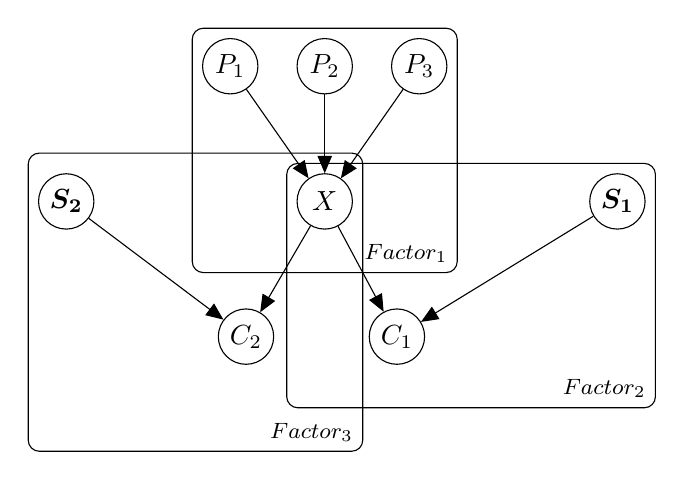
\begin{tikzpicture}

  % Define nodes
  \node[latent]                               (c1) {$C_2$};
  \node[latent, right= 1.2 cm of c1]            (c2) {$C_1$};
  \node[latent, above=of c1, xshift= 1 cm] (y)  {$X$};
  \node[latent, above=of y, xshift=-1.2cm] (p1) {$P_1$};
  \node[latent, above=of y, xshift=0cm]  (p2) {$P_2$};
  \node[latent, above=of y, xshift=1.2cm]  (p3) {$P_3$};
  \node[latent, right= 3.0cm of y]            (s1) {$\boldsymbol{S_1}$};
  \node[latent, right=-4.0cm of y]            (s2) {$\boldsymbol{S_2}$};

  % Connect the nodes
  \edge {p1,p2,p3} {y} ; %
  \edge {y,s1}{c2} ;
  \edge {y,s2}{c1};

  % Plates
  \plate {} {(p1)(p2)(p3)(y)} {$Factor_1$} ;
  \plate {yx} {(y)(s1)(c2)} {$Factor_2$};
  \plate {} {(y)(s2)(c1)(yx.north west)(yx.south west)} {$Factor_3$} ;
  %\plate {} {(w)(y)(yx.north west)(yx.south west)} {$M$} ;

\end{tikzpicture}
%\endpgfgraphicnamed

%%% Local Variables: 
%%% mode: tex-pdf
%%% TeX-master: "example"
%%% End: 

  \caption{Factorization of $P(_{-\cX} \mid \Lambda)$}
  \label{fig:example_factorization}
\end{figure}

The concept behind the factorization is also the motivation behind forward sampling in a Bayesian network.
The parents of $\cX$ are independent of the children given $\cX$.
The parents are not necessarily individually independent, and thus the parental term $P(D_{\Pa_{\cX}} \mid \Lambda)$ cannot be factored further.
The children of $\cX$ are similarly independent given $\cX$ and the corresponding spouses, leading to their factored product $\prod_{C_i} P(D_{C_i} \mid \Lambda, D_{\bm{S}_i})$.
Each component in the decomposition can be evaluated given a discretization policy and a dataset.

\subsubsection{Evaluation of $P\paren{D_{\Pa_{\cX}} \mid \Lambda}$}

Let $J_P$ be the number of instantiations of the parents of $\cX$, and let $n^{(\text{p})}_{i,j}$ be the number of instances of $\cX$ within the $i$th discretization interval of $\Lambda$ given the $j$th parental instantiation.
Note that $\gamma_i = \sum_j n^{(\text{p})}_{i,j}$.
It follows that

\begin{equation}
  \label{eq:likelihood_one}
  P\paren{D_{\Pa_{\cX}} \mid \Lambda} = \overbrace{\prod_{i=1}^k}^{\text{Principle 4}}
    \overbrace{\rule{0pt}{2em}
      \frac{1}{{{\gamma_i + J_P - 1}\choose{J_P - 1}}}
      \frac{1}{
        \frac{
          {\gamma_i}!
        }{
          {n^{({P})}_{i,1}}! \; {n^{({P})}_{i,2}}! \; \cdots \; {n^{({P})}_{i,J_P}}!
        }
      }
    }^{\text{Principle 2}}\text{.}
\end{equation}

The two factors on the right hand side comes from the second principle: all distributions of values of $\Pa_{\cX}$ in a given interval are equiprobable.
According to the fourth principle, the distribution in each interval is independent, so the two factors can be multiplied together.

\subsubsection{Evaluation of $P(D_{C_j} \mid \Lambda, D_{\bm{S}_j})$}
Let $J_{C_j}$ be the number of instantiations of the $j$th child of $\cX$, let $J_S^{(j)}$ be the number instantiations of the $j$th spouse set $\bm{S}_j$, and let $n^{(j)}_{i,m,l}$ be the number of instances of $\cX$ in the $i$th discretization interval of $\Lambda$ given the $m$th instantiation of $C_j$ and the $l$th instantiation of $\boldsymbol{S_j}$.
Let ${n^{(j)}_{i,l} = \sum_{m=1}^{J_j} n^{(j)}_{i,m,l}}$.
Note that ${\gamma_i = \sum_l n^{(j)}_{i,l}}$.
It follows that

\begin{equation}
  \label{eq:likelihood_two}
  P(D_{C_j} \mid \Lambda, D_{\bm{S}_j}) =
  \overbrace{\prod_{i=1}^{k} \prod_{l=1}^{J_S^{(j)}}}^{\text{Principle 4}}
    \overbrace{\rule{0pt}{2.3em}
      {
        \frac{1}{
          {{n^{(j)}_{i,l} + J_{C_j} - 1}\choose{J_{C_j}-1}}}
        }
        {\frac{
          1
        }{
          \frac{
            {n^{(j)}_{i,l}}!
          }{
            {n^{(j)}_{i,1,l}!} \; {n^{(j)}_{i,2,l}!} \; \cdots \; {n^{(j)}_{i,J_{C_j},l}!}
          }
        }
      }
    }^{\text{Principle 3}}
    \text{.}
\end{equation}

The two factors on the right hand side come from the third principle: all distribution of values of $C_j$ in a given interval and with a given value of $S_j$ are equiprobable.
According to the fourth prior, these distributions are independent from each other, and one can thus take their product.
If $\bm{S}_j = \emptyset$, then Equation~\ref{eq:likelihood_two} is equivalent to

\begin{equation}
  \label{eq:likelihood_three}
  P(D_{C_j} \mid \Lambda) =
  \overbrace{\prod_{i=1}^{k}}^{\text{Principle 4}}
  \overbrace{{
    {1}\over{
      {\gamma_i + J_{C_j} - 1}\choose{J_{C_j}-1}}
    }
    {{1}\over{
      {{\gamma_i}!} \over {
        {n^{(j)}_{i,1,\emptyset}!} \; {n^{(j)}_{i,2,\emptyset}!} \; \cdots \; {n^{(j)}_{i,J_{C_j},\emptyset} !}
      }
    }
  }}^{\text{Principle 3}}
  \text{,}
\end{equation}

\noindent
where $n^{(j)}_{i,m,\emptyset}$ is the number of instances of $\cX$ in the $i$th discretization interval of $\Lambda$ given the $m$th instantiation of $C_j$.

The objective function can be formulated given equations~\ref{eq:p_M},~\ref{eq:p_D_given_M},~\ref{eq:likelihood_one}, and~\ref{eq:likelihood_three}.
The log-inverse of $P(\Lambda) \cdot P(D_{-\cX} \mid \Lambda)$ is minimized for computational convenience:

\begin{equation}
\label{eq:opt_prob}
\begin{aligned}
  & \sum_{i=1}^{k-1}
   - \ln
    \paren{
      1 - \exp
      \paren{
        - L \cdot  \frac{
                         \cx_{\lambda_i +1} - \cx_{\lambda_i}
                       }{
                         \cx_n - \cx_1
                        }
      }
    }
      + \sum_{i=1}^{k}
      L \cdot \frac{\cx_{\lambda_{i}} - \cx_{\lambda_{i-1} + 1}}{\cx_n - \cx_1} \\
  & \sum_{i=1}^{k} \brock{
  \ln{{\gamma_i + J_P - 1}\choose{J_P - 1}}
  +{ \ln \paren{
        \frac{
          {\gamma_i}!
        }{
          {n^{({P})}_{i,1}}! \; {n^{({P})}_{i,2}}! \; \cdots \; {n^{({P})}_{i,J_P}}!
        }
      }}
  } \\
  & \sum_{j=1}^{n_c} \sum_{i=1}^k \sum_{l=1}^{J^{(j)}_S} \brock{
  { \ln
          {{n^{(j)}_{i,l} + J_{C_j} - 1}\choose{J_{C_j}-1}}}
    +
    \ln \paren{ {
          \frac{
            {n^{(j)}_{i,l}}!
          }{
            {n^{(j)}_{i,1,l}!} \; {n^{(j)}_{i,2,l}!} \; \cdots \; {n^{(j)}_{i,J_{C_j},l}!}
          }
        }
        } }
\end{aligned}
\end{equation}

All parameters and variables in the objective function are explained in previous subsections.

\subsection{Algorithm}

This section describes the procedure used to minimize the objective function.
Note that the objective function is cumulative over intervals, thus, if a partition of $X$ into $k$ intervals by $\Lambda = \curly{\gamma_1 , \gamma_2  , \ldots , \gamma_k}$ is an optimal discretization policy, then any subinterval is optimal for the corresponding subproblem.
It follows that dynamic programming can be used to solve the optimization problem exactly.

Precomputation reduces runtime.
Compute $h(u,v)$ for each interval $\gamma_q$ starting from $x_{u}$ to $x_{v}$ for all $u$, $v$ satisfying $u \leq v$:

\begin{small}
  \begin{equation}
  \begin{aligned}
  h(u,v) &=  \ln {{\gamma_{q} + J_P - 1}\choose{J_P-1}} + \ln \left( { {{\gamma_q}!}\over{ {n^{(p)}_{q,1} !} {n^{(p)}_{q,2} !} \cdots {n^{(p)}_{q,J_p} !}} } \right) \\
  & + \sum_{j=1}^{n_c} \sum_{l=1}^{J^{(j)}_S} \brock{
    { \ln
            {{n^{(j)}_{i,l} + J_{C_j} - 1}\choose{J_{C_j}-1}}}
      +
      \ln \paren{ {
            \frac{
              {n^{(j)}_{i,l}}!
            }{
              {n^{(j)}_{i,1,l}!} \; {n^{(j)}_{i,2,l}!} \; \cdots \; {n^{(j)}_{i,J_{C_j},l}!}
            }
          }
          } }
  \end{aligned}
  \end{equation}
\end{small}

The evaluation of $h(u,v)$ for all $u \leq v$ is summarized in Algorithm~\ref{alg:h} in the appendix.
\todo{The calculation has a $\bigo \paren{ n_c  {L'} \cdot N^2 + {L'}^{n_p} \cdot N^2 }$ runtime, where $n_c$ and $n_p$ are the numbers of child and parent variables respectively, and $L'$ is the largest cardinality of variables that directly connect to $X$.}

The optimization problem over Equation~\ref{eq:opt_prob} can now be solved.
The dynamic programming procedure is shown in Algorithm~\ref{alg:disc_one}.
It takes three inputs: $\cX$, the continuous variable; $D$, the joint data instances over all variables sorted in ascending order according to $D_X$; and $G$, the network structure.
The runtime of Algorithm~\ref{alg:disc_one} is also $O(n_c  {L'} \cdot N^2 + {L'}^{n_p} \cdot N^2)$, because the runtime of the dynamic programming procedure is less than the runtime for computing $h(u,v)$.
Algorithm~\ref{alg:disc_one} is guaranteed to be optimal.
For faster methods with suboptimal results please refer to the work of \cite{Boulle_2006}.

\begin{algorithm}
  \caption{Discretization of one continuous variable in a Bayesian network}
  \label{alg:disc_one}
  \begin{algorithmic}[5]
    \Function{DiscretizeOne}{$\cX$, $D$, $G$}
      \State $n \leftarrow$ the number of data instances
      \State $m \leftarrow$ the number of unique values in $D_{\cX}$
      \State $H \leftarrow$ an $N \times N$ matrix such that $H[u,v] = h(u,v)$ (see Algorithm~\ref{alg:h} in Appendix)
      \State $s_{1:m} \leftarrow$ an increasing sequence of integers defined in Section~\ref{subsec:disc_policy}
      \State $L \leftarrow$ the largest cardinality over all discrete variables in the Markov blanket of $X$
      \State $S[u] \leftarrow$ the optimal objective value of subproblems from instance $1$ to $s_u$
      \State $\Lambda[u] \leftarrow$ the optimal discretization for subproblems from instance $1$ to $s_u$
      \State $W[u]  \leftarrow - \ln\brock{1 - {\exp\paren{- L \cdot{ {{\cx_{s_u+1} - \cx_{s_u}}\over{\cx_n - \cx_1}}}}}}$ for $u = 1,2, \ldots,m-1$ and $W[n] \leftarrow 0$
      \For {$v \leftarrow 1$ to $m$}
        \If {$v = 1$}
          \State $S[v] \leftarrow H \paren{1,s_v} + L[v]$
          \State $\Lambda[v] \leftarrow \{ ({\cx_{s_v} + \cx_{s_v+1}}) / 2\}$
        \Else
          \State $s \leftarrow \infty$
          \State $\text{DiscEdge} \leftarrow \infty$
        \For {$u \leftarrow 1$ to $v$}
        \State $s' \leftarrow S[u] + H \paren{s_u+1, s_v} +  {L \cdot {\frac{\cx_{s_v} - \cx_{s_u + 1}}{\cx_n - \cx_1}}} + W[v]$
        \If {$s' < s$}
          \State $s \leftarrow s'$
          \State $\text{DiscEdge} \leftarrow ({x_{s_u} + x_{s_u+1}}) / 2$
        \EndIf
        \EndFor
          \State $S[v] \leftarrow s$
          \State $\Lambda[v] \leftarrow \Lambda[u] \cup \{ DiscEdge \}$
        \EndIf
      \EndFor
      \State \Return $\Lambda[m]$
    \EndFunction
  \end{algorithmic}
\end{algorithm}


\subsection{Approximation}

Algorithm~\ref{alg:disc_one} has an exponential $\bigo\paren{\paren{L'}^{n_p} \cdot N^2}$ runtime which severely limits discretization in networks with a large number of discretization intervals or parent variables.
This section introduces an approximation to the objective function that significantly reduces the runtime and still preserves the quality of discretization.
The approximation replaces the dominator of the last factor in Equation~\ref{eq:likelihood_one} with

\begin{equation}
{\frac{{\gamma_i}!}{ {n^{(P)}_{i,1} !} {n^{(P)}_{i,2} !} \cdots {n^{(P)}_{i,J_P} !}}} \approx \prod_{r=1}^{n_p} { {{{\gamma}_i}!}\over{ {n^{(P_r)}_{i,1} !} {n^{(P_r)}_{i,2} !} \cdots {n^{(P_r)}_{i,J_{P_r}} !}}}\text{,}
\end{equation}

\noindent
where $P_r$ is the $r$th parent variable, $J_{p_r} = \| P_r\|$, and ${n^{(P_r)}_{i,j} !}$ is the number of instances in the $i$th interval with the $j$th value of $P_r$. Note that $\gamma_i = \sum_j {n^{(P_r)}_{i,j}}$ for all $r$.
The approximated objective function is

\begin{small}
  \begin{equation}
  \label{eq:opt_prob_approx}
  \begin{aligned}
    & \sum_{i=1}^{k-1}
     - \ln
      \paren{
        1 - \exp
        \paren{
          - L \cdot  \frac{
                           \cx_{\lambda_i +1} - \cx_{\lambda_i}
                         }{
                           \cx_n - \cx_1
                          }
        }
      }
        + \sum_{i=1}^{k}
        L \cdot \frac{\cx_{\lambda_{i}} - \cx_{\lambda_{i-1} + 1}}{\cx_n - \cx_1} \\
    & \sum_{i=1}^{k} \brock{
    \ln{{\gamma_i + J_P - 1}\choose{J_P - 1}}
    +{ \ln \paren{
          \frac{
            {\gamma_i}!
          }{ \sum_{r=1}^{n_p}
            {n^{({P_r})}_{i,1}}! \; {n^{({P_r})}_{i,2}}! \; \cdots \; {n^{({P_r})}_{i,J_{P_r}}}!
          }
        }}
    } \\
    & \sum_{j=1}^{n_c} \sum_{i=1}^k \sum_{l=1}^{J^{(j)}_S} \brock{
    { \ln
            {{n^{(j)}_{i,l} + J_{C_j} - 1}\choose{J_{C_j}-1}}}
      +
      \ln \paren{ {
            \frac{
              {n^{(j)}_{i,l}}!
            }{
              {n^{(j)}_{i,1,l}!} \; {n^{(j)}_{i,2,l}!} \; \cdots \; {n^{(j)}_{i,J_{C_j},l}!}
            }
          }
          } }
  \end{aligned}
  \end{equation}
\end{small}

The approximation reduces the runtime of Algorithm~\ref{alg:disc_one} to a polynomial, $\todo{\bigo\paren{ {v'_\text{max}} \cdot (n_c + n_p) \cdot n^2}}$.
It will be shown in Section~\ref{sec:experiments} that the approximation is more sensitive to the distribution over other variables and is biased towards slightly higher interval counts.
\tim{We need to have a more specific thing to say along the lines of `When does it fail?'}

The approximated objective function, Equation~\ref{eq:opt_prob_approx}, provides intuition into how child and parent variables contribute to the objective function.
For example, in the left graph of Figure~\ref{fig:example_networks}, the corresponding square brackets in the approximated objective function are

\begin{small}
  \begin{equation}
  \begin{aligned}
  \label{eq:example_approx}
   \sum_{i=1}^k & \left\lbrace   \left[ \ln{{\gamma_{i} + J_{C_1} - 1}\choose{J_{C_1}-1}} + \ln \left(  {{{\gamma_i}!} \over { {n^{(1)}_{i,1,\emptyset} !} \cdots {n^{(1)}_{i,J_{C_1},\emptyset} !}} }  \right)  +  \right. \right.\\
  & \left.  \ln{{\gamma_{i} + J_{C_2} - 1}\choose{J_{C_2}-1}} + \ln \left(  {{{n_i}!} \over { {n^{(2)}_{i,1,\emptyset} !} \cdots {n^{(2)}_{i,J_{C_1},\emptyset} !}} }  \right)  \right] + \\
  &  \left. \left[  \ln {{\gamma_{i} + J_P - 1}\choose{J_P-1}} +  \ln \left( { {{{\gamma}_i}!}\over{ {n^{(P_1)}_{i,1} !}\cdots {n^{(P_1)}_{i,J_{P_1}} !}}} \right) +\ln \paren{{ {{{\gamma}_i}!}\over{ {n^{(P_2}_{i,1} !}\cdots {n^{(P_2)}_{i,J_{P_2}} !}}} } \right] \right\rbrace \text{.}
  \end{aligned}
  \end{equation}
\end{small}

In Equation~\ref{eq:example_approx}, each child carries two terms, as shown in the first set of square brackets, but the two parent variables only carry a total of three terms, as shown in the second set of square brackets.
In this case the child variables have greater effect on the optimal discretization than the parent variables, even though the number of child and parent variables are the same.
However, if $C_2$ has an additional parent $S_2$, as shown in the right graph of Figure~\ref{fig:example_networks}, the importances of $C_2$ will be reduced.
This is due to the additional influence of $S_2$ on $C_2$.
This phenomenon arrises because the Bayesian method, but with and without the heuristic, incorporates graph structure when discretizing continuous variables.

\begin{figure}[ht]
  \centering
  \begin{tabular}{cc}
    % model_pca.tex
%
% Copyright (C) 2012 Jaakko Luttinen
%
% This file may be distributed and/or modified
%
% 1. under the LaTeX Project Public License and/or
% 2. under the GNU General Public License.
%
% See the files LICENSE_LPPL and LICENSE_GPL for more details.

% PCA model

%\beginpgfgraphicnamed{model-pca}
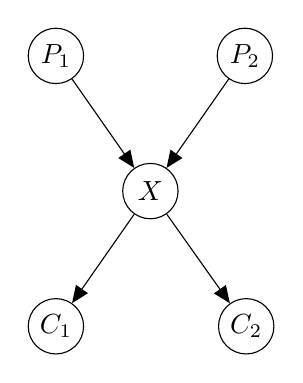
\begin{tikzpicture}

  % Define nodes
  \node[latent]                               (c1) {$C_1$};
  \node[latent, right= 1.7 cm of c1]            (c2) {$C_2$};
  \node[latent, above=of c1, xshift= 1.2 cm] (y)  {$X$};
  \node[latent, above=of y, xshift=-1.2cm] (p1) {$P_1$};
  \node[latent, above=of y, xshift=1.2cm]  (p2) {$P_2$};

  % Connect the nodes
  \edge {p1,p2} {y} ; %
  \edge {y} {c2} ;
  \edge {y}{c1};

  % Plates
  %\plate {} {(p1)(p2)(p3)(y)} {$Factor_1$} ;
  %\plate {yx} {(y)(s11)(s12)(c2)} {$Factor_2$};
  %\plate {} {(y)(s2)(c1)(yx.north west)(yx.south west)} {$Factor_3$} ;
  %\plate {} {(w)(y)(yx.north west)(yx.south west)} {$M$} ;

\end{tikzpicture}
%\endpgfgraphicnamed

%%% Local Variables: 
%%% mode: tex-pdf
%%% TeX-master: "example"
%%% End: 

    \end{tabular}
    \hspace{5em}
    \begin{tabular}{cc}
    % model_pca.tex
%
% Copyright (C) 2012 Jaakko Luttinen
%
% This file may be distributed and/or modified
%
% 1. under the LaTeX Project Public License and/or
% 2. under the GNU General Public License.
%
% See the files LICENSE_LPPL and LICENSE_GPL for more details.

% PCA model

%\beginpgfgraphicnamed{model-pca}
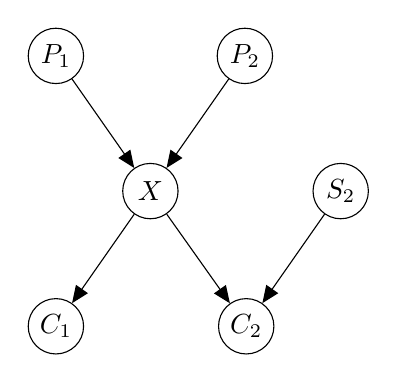
\begin{tikzpicture}

  % Define nodes
  \node[latent]                               (c1) {$C_1$};
  \node[latent, right= 1.7 cm of c1]            (c2) {$C_2$};
  \node[latent, above=of c1, xshift= 1.2 cm] (y)  {$X$};
  \node[latent, above=of c2, xshift= 1.2 cm] (s)  {$S_2$};
  \node[latent, above=of y, xshift=-1.2cm] (p1) {$P_1$};
  \node[latent, above=of y, xshift=1.2cm]  (p2) {$P_2$};

  % Connect the nodes
  \edge {p1,p2} {y} ; %
  \edge {y} {c2} ;
  \edge {y}{c1};
  \edge {s}{c2};

  % Plates
  %\plate {} {(p1)(p2)(p3)(y)} {$Factor_1$} ;
  %\plate {yx} {(y)(s11)(s12)(c2)} {$Factor_2$};
  %\plate {} {(y)(s2)(c1)(yx.north west)(yx.south west)} {$Factor_3$} ;
  %\plate {} {(w)(y)(yx.north west)(yx.south west)} {$M$} ;

\end{tikzpicture}
%\endpgfgraphicnamed

%%% Local Variables: 
%%% mode: tex-pdf
%%% TeX-master: "example"
%%% End: 

  \end{tabular}
  \caption{Two example networks}
  \label{fig:example_networks}
\end{figure}

%%%%%%%%%%%%%%%%%%%%%%%%%%%%%%%%%%%%%%%%%%%%%%%%%%%%%%%%%%%%%%%%%%%%%%%%%%%%%%%%%%%%%%

\section{Multi-Variable Discretization}
\label{sec:multi_var}

\subsection{Discretization of Multiple Continuous Variables}

The single-variable discretization method can be extended to Bayesian networks with multiple continuous variables by iteratively discretizing individual variables.
The discretization process for a single variable requires that all other variables be discrete.
The iterative approach uses a prediscretization policy in order to initialize the process.
This work prediscretizes all continuous variables into $k$ equal-width intervals, where $k$ is the median value of the number of intervals of initially discrete variables in the network.

After prediscretization, the one-variable discretization method is iteratively applied over each continuous variable in reverse topoligical order, from the leaves to the root.
Reverse topological order has the advantage of relying on fewer prediscretizations of the continuous variables during the first pass.
For example, in the right-hand graph of Figure~\ref{fig:example_networks}, assume $S_2$ is the only discrete variable.
The discretization of $P_1$ involves both $P_2$ and $\cX$, whereas the discretization of $C_1$ only involves $\cX$.

The algorithm is terminated when the number of discretization intervals and their associated edges converge for all variables, and a maximum number of complete passes is enforced to prevent infinite iterations when convergence does not occur.
The algorithm typically converges within a few passes when tested on real-world data.
In cases where it does not converge, \tim{only observed when also learning structure}, ten passes usually produce decent discretization results.

The pseudocode for the multi-variable discretization procedure is shown in Algorithm~\ref{alg:disc_two}.
It requires four inputs: $D$, a dataset of samples from the joint distribution; $G$, the fixed network structure; $\bm{\cX}$, the set of all continuous variables in reverse topological order, and $\maxpasses$, an upper bound on the number of complete passes.

\begin{algorithm}
  \caption{Discretization of multiple continuous variables}
  \label{alg:disc_two}
  \begin{algorithmic}[5]
  \Function{DiscretizeAll}{$D$, $G$, $\bm{\cX}$, $\maxpasses$}
    \State $\discset \leftarrow$ the discretization policies for each $\cX$ in $\bm{\cX}$
    \State $D^* \leftarrow $ the dataset $D$ discretized according to $\discset$
    \State $k \leftarrow \textsc{Median}\paren{\curly{ |X| \text{ s.t. } X \text{ does not have corresponding } \cX \text{ in } \bm{\cX} }}$
    \For {$\paren{\cX, X}$ such that $\cX \in \bm{\cX}$ and $X$ is the discretized version of $\cX$}
      \State $\Lambda_{\cX} \leftarrow$ equal-width discretization of $\cX$ with $k$ intervals
      \State $D^*_{X} \leftarrow \Lambda_{\cX} \paren{D_{\cX}}$
    \EndFor
    \State $n_\text{cycle} \leftarrow 0$
    \While {$\discset$ has not converged \textbf{and} $n_\text{cycle} \leq \maxpasses$}
      \State increment {$n_\text{cycle}$}
      \For {$\paren{\cX, X}$ such that $\cX \in \bm{\cX}$}
        \State {$D^*_X \leftarrow D_{\cX}$}
        \State {$\Lambda_{\cX} \leftarrow \textsc{DiscretizeOne}(\cX, D^*, G)$}
        \State {$D^*_X \leftarrow \Lambda_{\cX}\paren{D_{\cX}}$}
      \EndFor
    \EndWhile
    \State \Return $\discset$
  \EndFunction
  \end{algorithmic}
\end{algorithm}

\subsection{Combining Discretization with Structure Learning}

In many situations the network structure is not known in advance and must be learned from data.
Traditional Bayesian structure learning algorithms require discretized data, whereas the proposed discretization algorithm requires a known network structure.
This section combines the proposed discretization method with the K2 structure learning algorithm \citep{K2} in an interative fassion to simultaneously perform Bayesian structure learning and discretization of continuous variables.

The proposed algorithm alternates between K2 structure learning and discretization.
K2 is run on the discretized dataset corresponding to prediscretizations for all continuous variables.
The affected continuous variables are rediscretized every time an edge is added by K2.
The resulting discretization policies are used to update the discretized dataset, and the next step of the K2 algorithm is executed.
This cycle is repeated until the K2 algorithm reaches a local maximum.

This procedure is given in Algorithm~\ref{alg:structure_learn}.
It takes five inputs: $D$, a dataset of samples from the joint distribution; $\bm{\cX}$, the set of all continuous variables; $\texttt{order}$, a permutation of the variables in $D$; $\hat{n}_\text{parent}$, an upper bound on the number of parents per node; and $\maxpasses$, an upper bound on the number of complete passes.

\begin{algorithm}
  \caption{Learning a discrete-valued Bayesian network}
  \label{alg:structure_learn}
  \begin{algorithmic}[5]
  \Function{Learn\_DBN}{$D$, $C$, $order$, $u_{parent}$, $C$, $\maxpasses$}
    \State $m \leftarrow$ the number of variables in the Bayesian network
    \State $k \leftarrow median\{ \|v\|, v\notin C\}$
    \State $\Lambda^{(i)} \leftarrow$ the discretization policy for the continuous variable $X_i$
    \State $D^*_{X_i} \leftarrow \Lambda^{(i)} (D_{X_i})$, list of instances of $X_i$ discretized by $\Lambda^{(i)}$
    \State $D^* \leftarrow $ the discretized data for all variables, where $D^*_{X_j} \leftarrow D_{X_j}$ if $X_j \notin C$
    \State $G \leftarrow$ the initial edgeless graph structure
    \For {$i \leftarrow 1$ to $n$}
      \If {$X_i \in C$}
        \State $\Lambda^{(i)} \leftarrow$ equal-width discretization with $k$ intervals
        \State $D^*_{X_i} \leftarrow  \Lambda^{(i)} (D_{X_i})$
      \EndIf
    \EndFor
    \For {$i \leftarrow 1$ to $n$}
      \State $P_{old} \leftarrow g(X^*_i,\Pa^*_X)$ as Equation~\ref{eq:B_Score_one}
      \State OKToProceed $\leftarrow$ \textbf{true}
      \While {OKToProceed \textbf{and} $\|\Pa_{X_i}\| < u_{parent}$}
        \State $Y \leftarrow$ an element from the set $order[1:i] \backslash \Pa_X$
        \State $P_{new} \leftarrow g(X^*_i,\Pa^*_{X_i} \cup Y^*)$
        \If {$P_{new} > P_{old}$}
          \State $P_{old} \leftarrow P_{new}$
          \State $\Pa_{X_i} \leftarrow \Pa_{X_i} \cup Y $
          \State $C' \leftarrow$ sorting variables in $C$ by a reverse topological order of current $G$
          \State $\Lambda \leftarrow$ \textsc{DiscretizeAll}({$D$, $G$, $C'$, $\maxpasses$}): Algorithm~\ref{alg:disc_two}
          \State $D*_{X_i} \leftarrow \Lambda^{(i)}(D_{X_i})$ for all $i$
        \Else
          \State OKToProceed $\leftarrow$ \textbf{false}
        \EndIf
      \EndWhile
    \EndFor
    \State \Return $G$, $\Lambda$
  \EndFunction
  \end{algorithmic}
\end{algorithm}

The function $g$ in Algorithm~\ref{alg:structure_learn} computes a component of the Bayesian score (Equation~\ref{eq:BayesianScore}):

\begin{equation}
  \label{eq:B_Score_one}
  g\paren{X_i, \Pa_{X_i}} =  \sum_{j=1}^{q_i} \ln\paren{
    \frac{
      \Gamma\paren{\alpha_{ij}^{(0)}}
    }{
      \Gamma\paren{\alpha_{ij}^{(0)} + \beta_{ij}^{(0)}}
    }
  } + \sum_{k=1}^{r_i} \ln \paren{
    \frac{
      \Gamma\paren{\alpha_{ij}^{(k)} + \beta_{ij}^{(k)}}
    }{
      \Gamma\paren{\alpha_{ij}^{(k)}}
    }
  }\text{.}
\end{equation}

It is common practice to run K2 multiple times with different variable permutations and to then choose the structure with the highest score.
As such, Algorithm~\ref{alg:structure_learn} is run multiple times with different variable permutations and the discretized Bayesian network with the highest score is retaiend.

%%%%%%%%%%%%%%%%%%%%%%%%%%%%%%%%%%%%%%%%%%%%%%%%%%%%%%%%%%%%%%%%%%%%%%%%%%%%%%%%%%%%%%

\section{Experiments}
\label{sec:experiments}

This section describes experiments conducted to evaluate the proposed methods.
All experiments were run on datasets from the publically available University of California, Irvine machine learning repository \citep{Lichman_2013}.
Variables are labelled alphabetically in the order given on the dataset information webpage
In the figures that follow, shaded nodes correspond to initially discrete variables and the subscripts indicate the number of discrete instantiations.

Two experiments were conducted on each dataset.
The first experiment compares the performance of the optimal Bayesian discretization method, the heuristic Bayesian discretization method, and MDL on a known Bayesian network structure.
The structure was obtained by prediscretizing each continuous variable into $k$ uniform-width intervals, where $k$ is the median number of instantiations of the discrete variables, and using the structure with the highest Bayesian score from one thousand runs of the K2 algorithm with random variable orderings.
The second experiment compares the same methods applied when simultaneously discretizing and learning network structure.

The discretizations are compared using the mean cross validated log-likelihood of the data $D$ given the graph structure $G$ and discretization policies $\discset$.
The log-likelihood has two components,

\begin{equation}
\ln p(D\mid G, \discset) = \ln P(D^*\mid G) + \ln p(D\mid \discset, D^*)\text{,}
\end{equation}

\noindent
where $D$ is the original dataset and $D^*$ is the dataset discretized according to $\discset$.
The log-likelihood of the discretized dataset is the Bayesian score (Equation~\ref{eq:BayesianScore}) evaluated with a uniform prior over graph structures and a uniform Dirichlet prior ($\alpha_{ijk} = 1$ for all $i$, $j$, and $k$).
The log-likelihood of the original dataset given the discrete dataset is

\todo{
\begin{equation}
  \ln p\paren{D\mid \discset, D^*} = \sum_{i=1}^n
  1\curly{X_i \text{ orig. cont.}}
  \sum_{j=1}^{q_i} \sum_{k=1}^{r_i} m_{ijk} \ln\paren{
    \frac{
      1
    }{
      e^{\Lambda_{\cX_i}}_{k+1} - e^{\Lambda_{\cX_i}}_{k}
    }
  }\text{.}
\end{equation}
}

\noindent
The mean cross-validated log-likelihood is the mean log-likelihood on the witheld dataset among cross-validation folds.
Cross-validation directly estimates generalization error.
Ten folds were used in each experiment.

The optimal discretization policy for MDL is found with dynamic programming in a similar manner as with the Bayesian method.
For a Bayesian network with a single continuous variable $\cX$, the MDL objective function is

\begin{equation}
  \label{eqn:MDL}
  \todo{
  \begin{aligned}
  \frac{1}{2} \ln(n) \left\lbrace  \lvert \Pa_{X_i} \rvert (\lvert X_i \rvert - 1) +
   {\sum_{j,\cX_i \in \Pa_{X_i}}} \lvert \Pa_{X_j} \rvert (\lvert \cX_j \rvert - 1) \right\rbrace + \ln(\lvert {\cX_i} \rvert) \\
   + (N_i-1) H \paren{\frac{|X^*_i| - 1}{N_i -1}} -n \cdot \left[ I(X_i,\Pa_{X_i}) + {\sum_{j,\cX_i \in \Pa_{\cX_i}}} I(\cX_j, \Pa_{X_j}) \right]\text{,}
  \end{aligned}
  }
\end{equation}

where $I(A,B)$ is the mutual information between two discrete variables $A$ and $B$, ${H(p) = -p \ln(p) - (1-p) \ln(1-p)}$, and \todo{$X^*_i$ is the discretized version of the $i$th sample of $X$}.


\subsection{Auto MPG Dataset}
\label{subsec:auto}

The Auto MPG dataset contains variables related to the fuel consumption of automobiles in urban driving.
The dataset has \num{392} samples over eight variables, not including six instances with missing data.
Three variables are discrete: $B$, $G$, and $H$, with \num{5}, \num{13}, and \num{3} instantiations respectively.

\subsubsection{Discretization with fixed Structure}
\label{subsubsec:auto_exp1}

The Bayesian approaches and the MDL discretization method were tested on the Auto MPG data using the network network shown in Figure~\ref{fig:auto_graph_1}.
This structure was obtained by prediscretizing each continuous variable into five uniform-width intervals, where five is the median cardinality of the discrete variables, and then taking the structure with highest likelihood from one thousand runs of K2.

\begin{figure}[ht]
  \centering
   % model_pca.tex
%
% Copyright (C) 2012 Jaakko Luttinen
%
% This file may be distributed and/or modified
%
% 1. under the LaTeX Project Public License and/or
% 2. under the GNU General Public License.
%
% See the files LICENSE_LPPL and LICENSE_GPL for more details.

% PCA model

%\beginpgfgraphicnamed{model-pca}
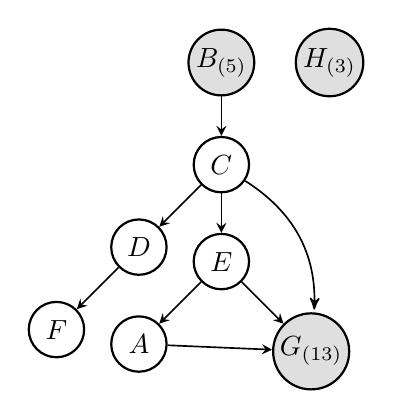
\begin{tikzpicture}[
      nodes={
        draw=black!20, thick, fill=white, font=\normalsize,
        minimum width=2.5em, minimum height=2em
      },
      rounded corners, semithick, >=stealth
      ]

      \node[obs]                 (c2) {$B_{{(5)}}$};
      \node[latent, below=0.5 of c2]   (c3){$C$};
      \node[latent, below=0.5 of c3]   (c5){$E$};
      \node[latent, below left = 0.75 of c3] (c4){$D$};
      \node[latent, below left = 0.75 of c4] (c6){$F$};
      \node[latent, below left = 0.75 of c5] (c1){$A$};
      \node[obs, below right = 0.75 of c5] (c7) {$G_{(13)}$};
      \node[obs, right = 0.5 of c2] (c8){$H_{{(3)}}$};


  % Connect the nodes
  \edge {c2}{c3};
  \edge {c3}{c4,c5};
  \draw[->,>=stealth', shorten >= 1pt] (c3) to[bend left](c7);
  \edge {c4}{c6};
  \edge {c5}{c1,c7};
  \edge {c1}{c7};
  %\edge {p1,p2} {y} ; %
  %\edge {y} {c2} ;
  %\edge {y}{c1};



\end{tikzpicture}
%\endpgfgraphicnamed

%%% Local Variables:
%%% mode: tex-pdf
%%% TeX-master: "example"
%%% End:

   \caption{Bayesian network structure obtained from running K2 on the prediscretized Auto MPG dataset}
  \label{fig:auto_graph_1}
\end{figure}

Table~\ref{table:auto_disc_table_1} lists the discretization edges and mean log-likelihoods under 10-fold cross validation of the discrete Bayesian network resulting from each discretization method.
The results indicate that the heuristic Bayesian method produces exactly the same discretization policy as the optimal Bayesian method.
The MDL method does not produce any discretization edges, assigning one continuous interval to each continuous variable, and produces the structure with the lowest score.
The cause behind MDL's discretization policy is discussed in Section~\ref{subsec:discuss_exp}.

\begin{table}[h]
  \centering
  \caption{
    Results from discretization of the Auto MPG dataset with fixed structure from Figure~\ref{fig:auto_graph_1}.
    The first five rows list the discretization edges for each continuous variable.
    The last row lists the mean cross-validated log-likelihood; positive values are better.
    The optimal and heuristic Bayesian discretization policies are identical and the MDL method does not produce any discretization edges.
  }
  \scriptsize
\begin{tabular}{cccc}
    \toprule
    Var. & Bayesian & Bayesian with Approximation & MDL \\
    \midrule
    $A$ & \numlist[list-final-separator = {, }]{15.25; 17.65; 20.90; 25.65; 28.90} & \numlist[list-final-separator = {, }]{15.25; 17.65; 20.90; 25.65; 28.90} & - \\
    $C$ & \numlist[list-final-separator = {, }]{70.5; 93.5; 109.0; 159.5; 259.0; 284.5} & \numlist[list-final-separator = {, }]{70.5;93.5;109.0;159.5;259.0;284.5} & - \\
    $D$ & \numlist[list-final-separator = {, }]{71.5;99.0;127.0} & \numlist[list-final-separator = {, }]{71.5;99.0; 127.0} & - \\
    $E$ & \numlist[list-final-separator = {, }]{2115;2481;2960;3658} & \numlist[list-final-separator = {, }]{2115;2481;2960;3658} & - \\
    $F$ & \numlist[list-final-separator = {, }]{12.35;13.75;16.05;22.85} & \numlist[list-final-separator = {, }]{12.35;13.75;16.05;22.85} & - \\
    \addlinespace[0.5em]
    Logl & \num{-10210} & \num{-10210} & \num{-11918} \\
    \bottomrule
\end{tabular}
  \label{table:auto_disc_table_1}
\end{table}

Figure~\ref{fig:auto_exp1_distr_1_3} compares the Bayesian discretizaton policy for variables $A$ and $C$ with the original Auto MPG data.
The black marks are the original Auto MPG samples.
The color of a discretized region indicates the marginal probability of a sample from $P(A,C)$ being drawn from that region.
As shown in the figure, the discretization edges obtained by the optimal Bayesian approach and the resulting marginalized probability match the raw data well.

\begin{figure}[ht]
\centering
  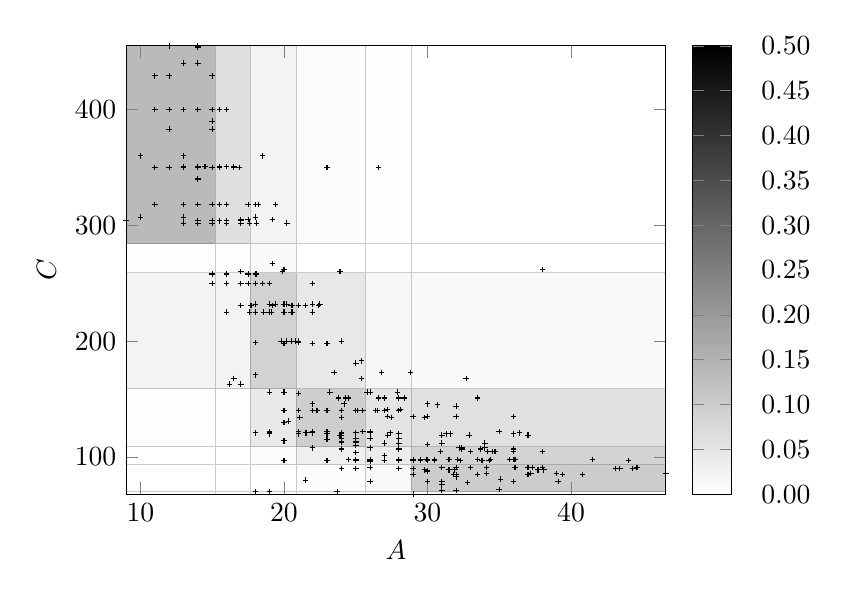
\begin{tikzpicture}
		\begin{axis}[
			view={0}{90},
			enlargelimits=0,
			zmin=0.0, zmax=1.0,
			xlabel=$A$,
			ylabel=$C$,
			colorbar,
			point meta min=0, point meta max=0.5,
			colormap={}{ gray(0cm)=(1); gray(1cm)=(0);},
			colorbar style={
			        ytick={0,0.05,...,0.51},
			        yticklabel style={
			            text width=2.5em,
			            align=right,
			            /pgf/number format/.cd,
			                fixed,
			                fixed zerofill
			        }
			    }
			]

			\addplot3[patch,shader=faceted,patch type=rectangle] coordinates {(9.0000,68.0000,0.0000) (15.2500,68.0000,0.0000) (15.2500,70.5000,0.0000) (9.0000,70.5000,0.0000)};
			\addplot3[patch,shader=faceted,patch type=rectangle] coordinates {(9.0000,70.5000,0.0000) (15.2500,70.5000,0.0000) (15.2500,93.5000,0.0000) (9.0000,93.5000,0.0000)};
			\addplot3[patch,shader=faceted,patch type=rectangle] coordinates {(9.0000,93.5000,0.0000) (15.2500,93.5000,0.0000) (15.2500,109.0000,0.0000) (9.0000,109.0000,0.0000)};
			\addplot3[patch,shader=faceted,patch type=rectangle] coordinates {(9.0000,109.0000,0.0020) (15.2500,109.0000,0.0020) (15.2500,159.5000,0.0020) (9.0000,159.5000,0.0020)};
			\addplot3[patch,shader=faceted,patch type=rectangle] coordinates {(9.0000,159.5000,0.0235) (15.2500,159.5000,0.0235) (15.2500,259.0000,0.0235) (9.0000,259.0000,0.0235)};
			\addplot3[patch,shader=faceted,patch type=rectangle] coordinates {(9.0000,259.0000,0.0030) (15.2500,259.0000,0.0030) (15.2500,284.5000,0.0030) (9.0000,284.5000,0.0030)};
			\addplot3[patch,shader=faceted,patch type=rectangle] coordinates {(9.0000,284.5000,0.1345) (15.2500,284.5000,0.1345) (15.2500,455.0000,0.1345) (9.0000,455.0000,0.1345)};

			\addplot3[patch,shader=faceted,patch type=rectangle] coordinates {(15.2500,68.0000,0.0000) (17.6500,68.0000,0.0000) (17.6500,70.5000,0.0000) (15.2500,70.5000,0.0000)};
			\addplot3[patch,shader=faceted,patch type=rectangle] coordinates {(15.2500,70.5000,0.0000) (17.6500,70.5000,0.0000) (17.6500,93.5000,0.0000) (15.2500,93.5000,0.0000)};
			\addplot3[patch,shader=faceted,patch type=rectangle] coordinates {(15.2500,93.5000,0.0000) (17.6500,93.5000,0.0000) (17.6500,109.0000,0.0000) (15.2500,109.0000,0.0000)};
			\addplot3[patch,shader=faceted,patch type=rectangle] coordinates {(15.2500,109.0000,0.0020) (17.6500,109.0000,0.0020) (17.6500,159.5000,0.0020) (15.2500,159.5000,0.0020)};
			\addplot3[patch,shader=faceted,patch type=rectangle] coordinates {(15.2500,159.5000,0.0230) (17.6500,159.5000,0.0230) (17.6500,259.0000,0.0230) (15.2500,259.0000,0.0230)};
			\addplot3[patch,shader=faceted,patch type=rectangle] coordinates {(15.2500,259.0000,0.0030) (17.6500,259.0000,0.0030) (17.6500,284.5000,0.0030) (15.2500,284.5000,0.0030)};
			\addplot3[patch,shader=faceted,patch type=rectangle] coordinates {(15.2500,284.5000,0.0625) (17.6500,284.5000,0.0625) (17.6500,455.0000,0.0625) (15.2500,455.0000,0.0625)};

			\addplot3[patch,shader=faceted,patch type=rectangle] coordinates {(17.6500,68.0000,0.0000) (20.9000,68.0000,0.0000) (20.9000,70.5000,0.0000) (17.6500,70.5000,0.0000)};
			\addplot3[patch,shader=faceted,patch type=rectangle] coordinates {(17.6500,70.5000,0.0000) (20.9000,70.5000,0.0000) (20.9000,93.5000,0.0000) (17.6500,93.5000,0.0000)};
			\addplot3[patch,shader=faceted,patch type=rectangle] coordinates {(17.6500,93.5000,0.0070) (20.9000,93.5000,0.0070) (20.9000,109.0000,0.0070) (17.6500,109.0000,0.0070)};
			\addplot3[patch,shader=faceted,patch type=rectangle] coordinates {(17.6500,109.0000,0.0430) (20.9000,109.0000,0.0430) (20.9000,159.5000,0.0430) (17.6500,159.5000,0.0430)};
			\addplot3[patch,shader=faceted,patch type=rectangle] coordinates {(17.6500,159.5000,0.0880) (20.9000,159.5000,0.0880) (20.9000,259.0000,0.0880) (17.6500,259.0000,0.0880)};
			\addplot3[patch,shader=faceted,patch type=rectangle] coordinates {(17.6500,259.0000,0.0095) (20.9000,259.0000,0.0095) (20.9000,284.5000,0.0095) (17.6500,284.5000,0.0095)};
			\addplot3[patch,shader=faceted,patch type=rectangle] coordinates {(17.6500,284.5000,0.0225) (20.9000,284.5000,0.0225) (20.9000,455.0000,0.0225) (17.6500,455.0000,0.0225)};

			\addplot3[patch,shader=faceted,patch type=rectangle] coordinates {(20.9000,68.0000,0.0015) (25.6500,68.0000,0.0015) (25.6500,70.5000,0.0015) (20.9000,70.5000,0.0015)};
			\addplot3[patch,shader=faceted,patch type=rectangle] coordinates {(20.9000,70.5000,0.0060) (25.6500,70.5000,0.0060) (25.6500,93.5000,0.0060) (20.9000,93.5000,0.0060)};
			\addplot3[patch,shader=faceted,patch type=rectangle] coordinates {(20.9000,93.5000,0.0320) (25.6500,93.5000,0.0320) (25.6500,109.0000,0.0320) (20.9000,109.0000,0.0320)};
			\addplot3[patch,shader=faceted,patch type=rectangle] coordinates {(20.9000,109.0000,0.0945) (25.6500,109.0000,0.0945) (25.6500,159.5000,0.0945) (20.9000,159.5000,0.0945)};
			\addplot3[patch,shader=faceted,patch type=rectangle] coordinates {(20.9000,159.5000,0.0455) (25.6500,159.5000,0.0455) (25.6500,259.0000,0.0455) (20.9000,259.0000,0.0455)};
			\addplot3[patch,shader=faceted,patch type=rectangle] coordinates {(20.9000,259.0000,0.0000) (25.6500,259.0000,0.0000) (25.6500,284.5000,0.0000) (20.9000,284.5000,0.0000)};
			\addplot3[patch,shader=faceted,patch type=rectangle] coordinates {(20.9000,284.5000,0.0070) (25.6500,284.5000,0.0070) (25.6500,455.0000,0.0070) (20.9000,455.0000,0.0070)};

			\addplot3[patch,shader=faceted,patch type=rectangle] coordinates {(25.6500,68.0000,0.0055) (28.9000,68.0000,0.0055) (28.9000,70.5000,0.0055) (25.6500,70.5000,0.0055)};
			\addplot3[patch,shader=faceted,patch type=rectangle] coordinates {(25.6500,70.5000,0.0110) (28.9000,70.5000,0.0110) (28.9000,93.5000,0.0110) (25.6500,93.5000,0.0110)};
			\addplot3[patch,shader=faceted,patch type=rectangle] coordinates {(25.6500,93.5000,0.0375) (28.9000,93.5000,0.0375) (28.9000,109.0000,0.0375) (25.6500,109.0000,0.0375)};
			\addplot3[patch,shader=faceted,patch type=rectangle] coordinates {(25.6500,109.0000,0.0545) (28.9000,109.0000,0.0545) (28.9000,159.5000,0.0545) (25.6500,159.5000,0.0545)};
			\addplot3[patch,shader=faceted,patch type=rectangle] coordinates {(25.6500,159.5000,0.0165) (28.9000,159.5000,0.0165) (28.9000,259.0000,0.0165) (25.6500,259.0000,0.0165)};
			\addplot3[patch,shader=faceted,patch type=rectangle] coordinates {(25.6500,259.0000,0.0000) (28.9000,259.0000,0.0000) (28.9000,284.5000,0.0000) (25.6500,284.5000,0.0000)};
			\addplot3[patch,shader=faceted,patch type=rectangle] coordinates {(25.6500,284.5000,0.0035) (28.9000,284.5000,0.0035) (28.9000,455.0000,0.0035) (25.6500,455.0000,0.0035)};

			\addplot3[patch,shader=faceted,patch type=rectangle] coordinates {(28.9000,68.0000,0.0030) (46.6000,68.0000,0.0030) (46.6000,70.5000,0.0030) (28.9000,70.5000,0.0030)};
			\addplot3[patch,shader=faceted,patch type=rectangle] coordinates {(28.9000,70.5000,0.0995) (46.6000,70.5000,0.0995) (46.6000,93.5000,0.0995) (28.9000,93.5000,0.0995)};
			\addplot3[patch,shader=faceted,patch type=rectangle] coordinates {(28.9000,93.5000,0.0860) (46.6000,93.5000,0.0860) (46.6000,109.0000,0.0860) (28.9000,109.0000,0.0860)};
			\addplot3[patch,shader=faceted,patch type=rectangle] coordinates {(28.9000,109.0000,0.0605) (46.6000,109.0000,0.0605) (46.6000,159.5000,0.0605) (28.9000,159.5000,0.0605)};
			\addplot3[patch,shader=faceted,patch type=rectangle] coordinates {(28.9000,159.5000,0.0120) (46.6000,159.5000,0.0120) (46.6000,259.0000,0.0120) (28.9000,259.0000,0.0120)};
			\addplot3[patch,shader=faceted,patch type=rectangle] coordinates {(28.9000,259.0000,0.0000) (46.6000,259.0000,0.0000) (46.6000,284.5000,0.0000) (28.9000,284.5000,0.0000)};
			\addplot3[patch,shader=faceted,patch type=rectangle] coordinates {(28.9000,284.5000,0.0005) (46.6000,284.5000,0.0005) (46.6000,455.0000,0.0005) (28.9000,455.0000,0.0005)};

			\addplot3[mark=+, draw=none, mark size=1.0] coordinates {
(18.000,307.000,1) (15.000,350.000,1) (18.000,318.000,1) (16.000,304.000,1) (17.000,302.000,1) (15.000,429.000,1) (14.000,454.000,1) (14.000,440.000,1) (14.000,455.000,1) (15.000,390.000,1) (15.000,383.000,1) (14.000,340.000,1) (15.000,400.000,1) (14.000,455.000,1) (24.000,113.000,1) (22.000,198.000,1) (18.000,199.000,1) (21.000,200.000,1) (27.000,97.000,1) (26.000,97.000,1) (25.000,110.000,1) (24.000,107.000,1) (25.000,104.000,1) (26.000,121.000,1) (21.000,199.000,1) (10.000,360.000,1) (10.000,307.000,1) (11.000,318.000,1) (9.000,304.000,1) (27.000,97.000,1) (28.000,140.000,1) (25.000,113.000,1) (19.000,232.000,1) (16.000,225.000,1) (17.000,250.000,1) (19.000,250.000,1) (18.000,232.000,1) (14.000,350.000,1) (14.000,400.000,1) (14.000,351.000,1) (14.000,318.000,1) (12.000,383.000,1) (13.000,400.000,1) (13.000,400.000,1) (18.000,258.000,1) (22.000,140.000,1) (19.000,250.000,1) (18.000,250.000,1) (23.000,122.000,1) (28.000,116.000,1) (30.000,79.000,1) (30.000,88.000,1) (31.000,71.000,1) (35.000,72.000,1) (27.000,97.000,1) (26.000,91.000,1) (24.000,113.000,1) (25.000,97.500,1) (23.000,97.000,1) (20.000,140.000,1) (21.000,122.000,1) (13.000,350.000,1) (14.000,400.000,1) (15.000,318.000,1) (14.000,351.000,1) (17.000,304.000,1) (11.000,429.000,1) (13.000,350.000,1) (12.000,350.000,1) (13.000,400.000,1) (19.000,70.000,1) (15.000,304.000,1) (13.000,307.000,1) (13.000,302.000,1) (14.000,318.000,1) (18.000,121.000,1) (22.000,121.000,1) (21.000,120.000,1) (26.000,96.000,1) (22.000,122.000,1) (28.000,97.000,1) (23.000,120.000,1) (28.000,98.000,1) (27.000,97.000,1) (13.000,350.000,1) (14.000,304.000,1) (13.000,350.000,1) (14.000,302.000,1) (15.000,318.000,1) (12.000,429.000,1) (13.000,400.000,1) (13.000,351.000,1) (14.000,318.000,1) (13.000,440.000,1) (12.000,455.000,1) (13.000,360.000,1) (18.000,225.000,1) (16.000,250.000,1) (18.000,232.000,1) (18.000,250.000,1) (23.000,198.000,1) (26.000,97.000,1) (11.000,400.000,1) (12.000,400.000,1) (13.000,360.000,1) (12.000,350.000,1) (18.000,232.000,1) (20.000,97.000,1) (21.000,140.000,1) (22.000,108.000,1) (18.000,70.000,1) (19.000,122.000,1) (21.000,155.000,1) (26.000,98.000,1) (15.000,350.000,1) (16.000,400.000,1) (29.000,68.000,1) (24.000,116.000,1) (20.000,114.000,1) (19.000,121.000,1) (15.000,318.000,1) (24.000,121.000,1) (20.000,156.000,1) (11.000,350.000,1) (20.000,198.000,1) (19.000,232.000,1) (15.000,250.000,1) (31.000,79.000,1) (26.000,122.000,1) (32.000,71.000,1) (25.000,140.000,1) (16.000,250.000,1) (16.000,258.000,1) (18.000,225.000,1) (16.000,302.000,1) (13.000,350.000,1) (14.000,318.000,1) (14.000,302.000,1) (14.000,304.000,1) (29.000,98.000,1) (26.000,79.000,1) (26.000,97.000,1) (31.000,76.000,1) (32.000,83.000,1) (28.000,90.000,1) (24.000,90.000,1) (26.000,116.000,1) (24.000,120.000,1) (26.000,108.000,1) (31.000,79.000,1) (19.000,225.000,1) (18.000,250.000,1) (15.000,250.000,1) (15.000,250.000,1) (16.000,400.000,1) (15.000,350.000,1) (16.000,318.000,1) (14.000,351.000,1) (17.000,231.000,1) (16.000,250.000,1) (15.000,258.000,1) (18.000,225.000,1) (21.000,231.000,1) (20.000,262.000,1) (13.000,302.000,1) (29.000,97.000,1) (23.000,140.000,1) (20.000,232.000,1) (23.000,140.000,1) (24.000,134.000,1) (25.000,90.000,1) (24.000,119.000,1) (18.000,171.000,1) (29.000,90.000,1) (19.000,232.000,1) (23.000,115.000,1) (23.000,120.000,1) (22.000,121.000,1) (25.000,121.000,1) (33.000,91.000,1) (28.000,107.000,1) (25.000,116.000,1) (25.000,140.000,1) (26.000,98.000,1) (27.000,101.000,1) (17.500,305.000,1) (16.000,318.000,1) (15.500,304.000,1) (14.500,351.000,1) (22.000,225.000,1) (22.000,250.000,1) (24.000,200.000,1) (22.500,232.000,1) (29.000,85.000,1) (24.500,98.000,1) (29.000,90.000,1) (33.000,91.000,1) (20.000,225.000,1) (18.000,250.000,1) (18.500,250.000,1) (17.500,258.000,1) (29.500,97.000,1) (32.000,85.000,1) (28.000,97.000,1) (26.500,140.000,1) (20.000,130.000,1) (13.000,318.000,1) (19.000,120.000,1) (19.000,156.000,1) (16.500,168.000,1) (16.500,350.000,1) (13.000,350.000,1) (13.000,302.000,1) (13.000,318.000,1) (31.500,98.000,1) (30.000,111.000,1) (36.000,79.000,1) (25.500,122.000,1) (33.500,85.000,1) (17.500,305.000,1) (17.000,260.000,1) (15.500,318.000,1) (15.000,302.000,1) (17.500,250.000,1) (20.500,231.000,1) (19.000,225.000,1) (18.500,250.000,1) (16.000,400.000,1) (15.500,350.000,1) (15.500,400.000,1) (16.000,351.000,1) (29.000,97.000,1) (24.500,151.000,1) (26.000,97.000,1) (25.500,140.000,1) (30.500,98.000,1) (33.500,98.000,1) (30.000,97.000,1) (30.500,97.000,1) (22.000,146.000,1) (21.500,121.000,1) (21.500,80.000,1) (43.100,90.000,1) (36.100,98.000,1) (32.800,78.000,1) (39.400,85.000,1) (36.100,91.000,1) (19.900,260.000,1) (19.400,318.000,1) (20.200,302.000,1) (19.200,231.000,1) (20.500,200.000,1) (20.200,200.000,1) (25.100,140.000,1) (20.500,225.000,1) (19.400,232.000,1) (20.600,231.000,1) (20.800,200.000,1) (18.600,225.000,1) (18.100,258.000,1) (19.200,305.000,1) (17.700,231.000,1) (18.100,302.000,1) (17.500,318.000,1) (30.000,98.000,1) (27.500,134.000,1) (27.200,119.000,1) (30.900,105.000,1) (21.100,134.000,1) (23.200,156.000,1) (23.800,151.000,1) (23.900,119.000,1) (20.300,131.000,1) (17.000,163.000,1) (21.600,121.000,1) (16.200,163.000,1) (31.500,89.000,1) (29.500,98.000,1) (21.500,231.000,1) (19.800,200.000,1) (22.300,140.000,1) (20.200,232.000,1) (20.600,225.000,1) (17.000,305.000,1) (17.600,302.000,1) (16.500,351.000,1) (18.200,318.000,1) (16.900,350.000,1) (15.500,351.000,1) (19.200,267.000,1) (18.500,360.000,1) (31.900,89.000,1) (34.100,86.000,1) (35.700,98.000,1) (27.400,121.000,1) (25.400,183.000,1) (23.000,350.000,1) (27.200,141.000,1) (23.900,260.000,1) (34.200,105.000,1) (34.500,105.000,1) (31.800,85.000,1) (37.300,91.000,1) (28.400,151.000,1) (28.800,173.000,1) (26.800,173.000,1) (33.500,151.000,1) (41.500,98.000,1) (38.100,89.000,1) (32.100,98.000,1) (37.200,86.000,1) (28.000,151.000,1) (26.400,140.000,1) (24.300,151.000,1) (19.100,225.000,1) (34.300,97.000,1) (29.800,134.000,1) (31.300,120.000,1) (37.000,119.000,1) (32.200,108.000,1) (46.600,86.000,1) (27.900,156.000,1) (40.800,85.000,1) (44.300,90.000,1) (43.400,90.000,1) (36.400,121.000,1) (30.000,146.000,1) (44.600,91.000,1) (33.800,97.000,1) (29.800,89.000,1) (32.700,168.000,1) (23.700,70.000,1) (35.000,122.000,1) (32.400,107.000,1) (27.200,135.000,1) (26.600,151.000,1) (25.800,156.000,1) (23.500,173.000,1) (30.000,135.000,1) (39.100,79.000,1) (39.000,86.000,1) (35.100,81.000,1) (32.300,97.000,1) (37.000,85.000,1) (37.700,89.000,1) (34.100,91.000,1) (34.700,105.000,1) (34.400,98.000,1) (29.900,98.000,1) (33.000,105.000,1) (33.700,107.000,1) (32.400,108.000,1) (32.900,119.000,1) (31.600,120.000,1) (28.100,141.000,1) (30.700,145.000,1) (25.400,168.000,1) (24.200,146.000,1) (22.400,231.000,1) (26.600,350.000,1) (20.200,200.000,1) (17.600,225.000,1) (28.000,112.000,1) (27.000,112.000,1) (34.000,112.000,1) (31.000,112.000,1) (29.000,135.000,1) (27.000,151.000,1) (24.000,140.000,1) (36.000,105.000,1) (37.000,91.000,1) (31.000,91.000,1) (38.000,105.000,1) (36.000,98.000,1) (36.000,120.000,1) (36.000,107.000,1) (34.000,108.000,1) (38.000,91.000,1) (32.000,91.000,1) (38.000,91.000,1) (25.000,181.000,1) (38.000,262.000,1) (26.000,156.000,1) (22.000,232.000,1) (32.000,144.000,1) (36.000,135.000,1) (27.000,151.000,1) (27.000,140.000,1) (44.000,97.000,1) (32.000,135.000,1) (28.000,120.000,1) (31.000,119.000,1) };
		\end{axis}
	\end{tikzpicture}

  \caption{
    Comparison of the Bayesian discretization policy for variables $A$ and $C$ to the original Auto MPG data learned with a fixed network.
    The marginal probabilities of discretized regions closely match the raw data.
  }
  \label{fig:auto_exp1_distr_1_3}
\end{figure}

\subsubsection{Discretization while Learning Structure}
\label{subsubsec:auto_exp2}

In this experiment the network structure was not fixed in advance and was learned simultaneously with the discretization policies.
Figure~\ref{fig:auto_graph_2} shows a learned Bayesian network structure and the corresponding numbers of intervals after discretization for each continuous variable.
This result was obtained by running Algorithm~\ref{alg:structure_learn} fifty times using the optimal Bayesian method and choosing the structure with the highest likelihood.

\begin{figure}[ht]
  \centering
  % model_pca.tex
%
% Copyright (C) 2012 Jaakko Luttinen
%
% This file may be distributed and/or modified
%
% 1. under the LaTeX Project Public License and/or
% 2. under the GNU General Public License.
%
% See the files LICENSE_LPPL and LICENSE_GPL for more details.

% PCA model

%\beginpgfgraphicnamed{model-pca}
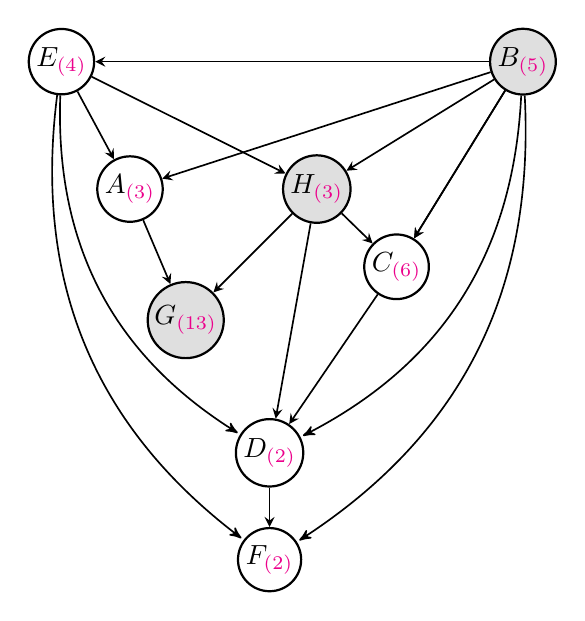
\begin{tikzpicture}[
      nodes={
        draw=black!20, thick, fill=white, font=\normalsize,
        minimum width=2.5em, minimum height=2em
      },
      rounded corners, semithick, >=stealth
      ]

      \node[obs]                 (c2) {$B_{\todo{(5)}}$};
      \node[latent, below left = 2.0 and 1.0 of c2]   (c3){$C_{\todo{(6)}}$};
      \node[latent, left =5.0 of c2]   (c5){$E_{\todo{(4)}}$};
      \node[latent, below left = 1.75 and 1.0 of c3] (c4){$D_{\todo{(2)}}$};
      \node[obs, below left = 1.0 and 2.0 of c2] (c8){$H_{\todo{(3)}}$};
      \node[latent, below = 0.5 of c4] (c6){$F_{\todo{(2)}}$};
      \node[latent, left = 1.5 of c8] (c1){$A_{\todo{(3)}}$};
      \node[obs, below left = 1.0  and 1.0 of c8] (c7) {$G_{\todo{(13)}}$};
      


  % Connect the nodes
  \edge {c2}{c3,c5,c1,c8,c3};
  \draw[->,>=stealth', shorten >= 1pt] (c2) to[bend left](c4);
  \draw[->,>=stealth', shorten >= 1pt] (c2) to[bend left](c6);
  \edge {c5}{c1,c8};
  \draw[->,>=stealth', shorten >= 1pt] (c5) to[bend right](c4);
  \draw[->,>=stealth', shorten >= 1pt] (c5) to[bend right](c6);
  \edge {c8}{c7,c4,c3};
  \edge {c1}{c7};
  \edge {c3}{c4};
  \edge {c4}{c6};
  %\draw[->,>=stealth', shorten >= 1pt] (c3) to[bend left](c7);
  %\edge {c4}{c6};
  %\edge {c5}{c1,c7};
  %\edge {c1}{c7};
  %\edge {p1,p2} {y} ; %
  %\edge {y} {c2} ;
  %\edge {y}{c1};



\end{tikzpicture}
%\endpgfgraphicnamed

%%% Local Variables: 
%%% mode: tex-pdf
%%% TeX-master: "example"
%%% End: 

  \caption{The discrete-valued Bayesian network learned from the Auto MPG dataset}
  \label{fig:auto_graph_2}
\end{figure}

Figure~\ref{fig:auto_exp2_distr_1_3} compares the Bayesian discretizaton policy for variables $A$ and $C$ in the learned network with the original Auto MPG data.
The color of a discretized region indicates the marginal probability of a sample from $P(A,C)$ being drawn from that region.
Although there are fewer discretization edges for $A$ and $C$ in the learned network, the marginal distribution is still captured.
Although the discretization result of the optimal Bayesian approach may vary according to the network structure, it still produces high-quality discretizations.

\begin{figure}[ht]
  \centering
  	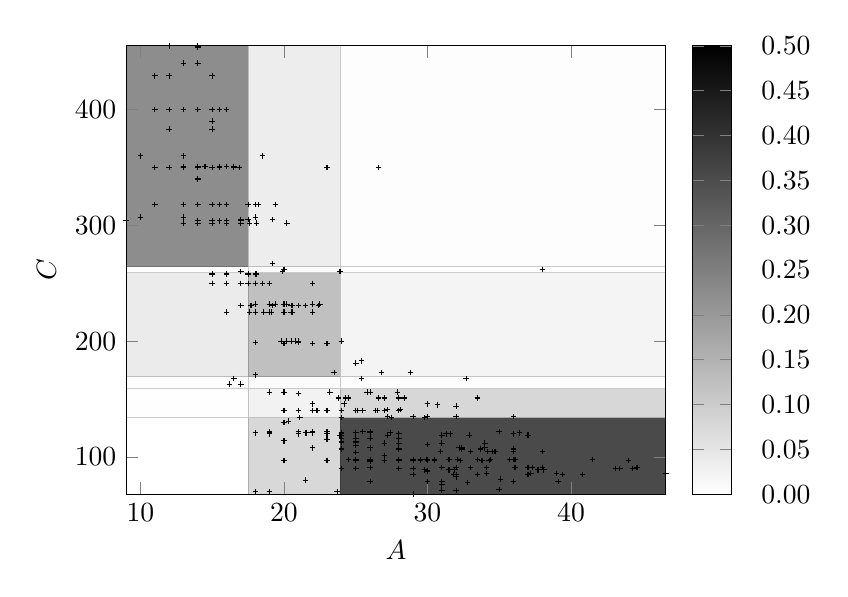
\begin{tikzpicture}
		\begin{axis}[
			view={0}{90},
			enlargelimits=0,
			zmin=0.0, zmax=1.0,
			xlabel=$A$,
			ylabel=$C$,
			colorbar,
			point meta min=0, point meta max=0.5,
			colormap={}{ gray(0cm)=(1); gray(1cm)=(0);},
			colorbar style={
			        ytick={0,0.05,...,0.51},
			        yticklabel style={
			            text width=2.5em,
			            align=right,
			            /pgf/number format/.cd,
			                fixed,
			                fixed zerofill
			        }
			    }
			]

			\addplot3[patch,shader=faceted,patch type=rectangle] coordinates {(9.0000,68.0000,0.0000) (17.5500,68.0000,0.0000) (17.5500,134.5000,0.0000) (9.0000,134.5000,0.0000)};
			\addplot3[patch,shader=faceted,patch type=rectangle] coordinates {(9.0000,134.5000,0.0010) (17.5500,134.5000,0.0010) (17.5500,159.5000,0.0010) (9.0000,159.5000,0.0010)};
			\addplot3[patch,shader=faceted,patch type=rectangle] coordinates {(9.0000,159.5000,0.0010) (17.5500,159.5000,0.0010) (17.5500,169.5000,0.0010) (9.0000,169.5000,0.0010)};
			\addplot3[patch,shader=faceted,patch type=rectangle] coordinates {(9.0000,169.5000,0.0395) (17.5500,169.5000,0.0395) (17.5500,259.0000,0.0395) (9.0000,259.0000,0.0395)};
			\addplot3[patch,shader=faceted,patch type=rectangle] coordinates {(9.0000,259.0000,0.0045) (17.5500,259.0000,0.0045) (17.5500,264.5000,0.0045) (9.0000,264.5000,0.0045)};
			\addplot3[patch,shader=faceted,patch type=rectangle] coordinates {(9.0000,264.5000,0.2220) (17.5500,264.5000,0.2220) (17.5500,455.0000,0.2220) (9.0000,455.0000,0.2220)};

			\addplot3[patch,shader=faceted,patch type=rectangle] coordinates {(17.5500,68.0000,0.0765) (23.9500,68.0000,0.0765) (23.9500,134.5000,0.0765) (17.5500,134.5000,0.0765)};
			\addplot3[patch,shader=faceted,patch type=rectangle] coordinates {(17.5500,134.5000,0.0260) (23.9500,134.5000,0.0260) (23.9500,159.5000,0.0260) (17.5500,159.5000,0.0260)};
			\addplot3[patch,shader=faceted,patch type=rectangle] coordinates {(17.5500,159.5000,0.0085) (23.9500,159.5000,0.0085) (23.9500,169.5000,0.0085) (17.5500,169.5000,0.0085)};
			\addplot3[patch,shader=faceted,patch type=rectangle] coordinates {(17.5500,169.5000,0.1225) (23.9500,169.5000,0.1225) (23.9500,259.0000,0.1225) (17.5500,259.0000,0.1225)};
			\addplot3[patch,shader=faceted,patch type=rectangle] coordinates {(17.5500,259.0000,0.0070) (23.9500,259.0000,0.0070) (23.9500,264.5000,0.0070) (17.5500,264.5000,0.0070)};
			\addplot3[patch,shader=faceted,patch type=rectangle] coordinates {(17.5500,264.5000,0.0355) (23.9500,264.5000,0.0355) (23.9500,455.0000,0.0355) (17.5500,455.0000,0.0355)};

			\addplot3[patch,shader=faceted,patch type=rectangle] coordinates {(23.9500,68.0000,0.3525) (46.6000,68.0000,0.3525) (46.6000,134.5000,0.3525) (23.9500,134.5000,0.3525)};
			\addplot3[patch,shader=faceted,patch type=rectangle] coordinates {(23.9500,134.5000,0.0770) (46.6000,134.5000,0.0770) (46.6000,159.5000,0.0770) (23.9500,159.5000,0.0770)};
			\addplot3[patch,shader=faceted,patch type=rectangle] coordinates {(23.9500,159.5000,0.0020) (46.6000,159.5000,0.0020) (46.6000,169.5000,0.0020) (23.9500,169.5000,0.0020)};
			\addplot3[patch,shader=faceted,patch type=rectangle] coordinates {(23.9500,169.5000,0.0210) (46.6000,169.5000,0.0210) (46.6000,259.0000,0.0210) (23.9500,259.0000,0.0210)};
			\addplot3[patch,shader=faceted,patch type=rectangle] coordinates {(23.9500,259.0000,0.0000) (46.6000,259.0000,0.0000) (46.6000,264.5000,0.0000) (23.9500,264.5000,0.0000)};
			\addplot3[patch,shader=faceted,patch type=rectangle] coordinates {(23.9500,264.5000,0.0035) (46.6000,264.5000,0.0035) (46.6000,455.0000,0.0035) (23.9500,455.0000,0.0035)};

			\addplot3[mark=+, draw=none, mark size=1.0] coordinates {
(18.000,307.000,1) (15.000,350.000,1) (18.000,318.000,1) (16.000,304.000,1) (17.000,302.000,1) (15.000,429.000,1) (14.000,454.000,1) (14.000,440.000,1) (14.000,455.000,1) (15.000,390.000,1) (15.000,383.000,1) (14.000,340.000,1) (15.000,400.000,1) (14.000,455.000,1) (24.000,113.000,1) (22.000,198.000,1) (18.000,199.000,1) (21.000,200.000,1) (27.000,97.000,1) (26.000,97.000,1) (25.000,110.000,1) (24.000,107.000,1) (25.000,104.000,1) (26.000,121.000,1) (21.000,199.000,1) (10.000,360.000,1) (10.000,307.000,1) (11.000,318.000,1) (9.000,304.000,1) (27.000,97.000,1) (28.000,140.000,1) (25.000,113.000,1) (19.000,232.000,1) (16.000,225.000,1) (17.000,250.000,1) (19.000,250.000,1) (18.000,232.000,1) (14.000,350.000,1) (14.000,400.000,1) (14.000,351.000,1) (14.000,318.000,1) (12.000,383.000,1) (13.000,400.000,1) (13.000,400.000,1) (18.000,258.000,1) (22.000,140.000,1) (19.000,250.000,1) (18.000,250.000,1) (23.000,122.000,1) (28.000,116.000,1) (30.000,79.000,1) (30.000,88.000,1) (31.000,71.000,1) (35.000,72.000,1) (27.000,97.000,1) (26.000,91.000,1) (24.000,113.000,1) (25.000,97.500,1) (23.000,97.000,1) (20.000,140.000,1) (21.000,122.000,1) (13.000,350.000,1) (14.000,400.000,1) (15.000,318.000,1) (14.000,351.000,1) (17.000,304.000,1) (11.000,429.000,1) (13.000,350.000,1) (12.000,350.000,1) (13.000,400.000,1) (19.000,70.000,1) (15.000,304.000,1) (13.000,307.000,1) (13.000,302.000,1) (14.000,318.000,1) (18.000,121.000,1) (22.000,121.000,1) (21.000,120.000,1) (26.000,96.000,1) (22.000,122.000,1) (28.000,97.000,1) (23.000,120.000,1) (28.000,98.000,1) (27.000,97.000,1) (13.000,350.000,1) (14.000,304.000,1) (13.000,350.000,1) (14.000,302.000,1) (15.000,318.000,1) (12.000,429.000,1) (13.000,400.000,1) (13.000,351.000,1) (14.000,318.000,1) (13.000,440.000,1) (12.000,455.000,1) (13.000,360.000,1) (18.000,225.000,1) (16.000,250.000,1) (18.000,232.000,1) (18.000,250.000,1) (23.000,198.000,1) (26.000,97.000,1) (11.000,400.000,1) (12.000,400.000,1) (13.000,360.000,1) (12.000,350.000,1) (18.000,232.000,1) (20.000,97.000,1) (21.000,140.000,1) (22.000,108.000,1) (18.000,70.000,1) (19.000,122.000,1) (21.000,155.000,1) (26.000,98.000,1) (15.000,350.000,1) (16.000,400.000,1) (29.000,68.000,1) (24.000,116.000,1) (20.000,114.000,1) (19.000,121.000,1) (15.000,318.000,1) (24.000,121.000,1) (20.000,156.000,1) (11.000,350.000,1) (20.000,198.000,1) (19.000,232.000,1) (15.000,250.000,1) (31.000,79.000,1) (26.000,122.000,1) (32.000,71.000,1) (25.000,140.000,1) (16.000,250.000,1) (16.000,258.000,1) (18.000,225.000,1) (16.000,302.000,1) (13.000,350.000,1) (14.000,318.000,1) (14.000,302.000,1) (14.000,304.000,1) (29.000,98.000,1) (26.000,79.000,1) (26.000,97.000,1) (31.000,76.000,1) (32.000,83.000,1) (28.000,90.000,1) (24.000,90.000,1) (26.000,116.000,1) (24.000,120.000,1) (26.000,108.000,1) (31.000,79.000,1) (19.000,225.000,1) (18.000,250.000,1) (15.000,250.000,1) (15.000,250.000,1) (16.000,400.000,1) (15.000,350.000,1) (16.000,318.000,1) (14.000,351.000,1) (17.000,231.000,1) (16.000,250.000,1) (15.000,258.000,1) (18.000,225.000,1) (21.000,231.000,1) (20.000,262.000,1) (13.000,302.000,1) (29.000,97.000,1) (23.000,140.000,1) (20.000,232.000,1) (23.000,140.000,1) (24.000,134.000,1) (25.000,90.000,1) (24.000,119.000,1) (18.000,171.000,1) (29.000,90.000,1) (19.000,232.000,1) (23.000,115.000,1) (23.000,120.000,1) (22.000,121.000,1) (25.000,121.000,1) (33.000,91.000,1) (28.000,107.000,1) (25.000,116.000,1) (25.000,140.000,1) (26.000,98.000,1) (27.000,101.000,1) (17.500,305.000,1) (16.000,318.000,1) (15.500,304.000,1) (14.500,351.000,1) (22.000,225.000,1) (22.000,250.000,1) (24.000,200.000,1) (22.500,232.000,1) (29.000,85.000,1) (24.500,98.000,1) (29.000,90.000,1) (33.000,91.000,1) (20.000,225.000,1) (18.000,250.000,1) (18.500,250.000,1) (17.500,258.000,1) (29.500,97.000,1) (32.000,85.000,1) (28.000,97.000,1) (26.500,140.000,1) (20.000,130.000,1) (13.000,318.000,1) (19.000,120.000,1) (19.000,156.000,1) (16.500,168.000,1) (16.500,350.000,1) (13.000,350.000,1) (13.000,302.000,1) (13.000,318.000,1) (31.500,98.000,1) (30.000,111.000,1) (36.000,79.000,1) (25.500,122.000,1) (33.500,85.000,1) (17.500,305.000,1) (17.000,260.000,1) (15.500,318.000,1) (15.000,302.000,1) (17.500,250.000,1) (20.500,231.000,1) (19.000,225.000,1) (18.500,250.000,1) (16.000,400.000,1) (15.500,350.000,1) (15.500,400.000,1) (16.000,351.000,1) (29.000,97.000,1) (24.500,151.000,1) (26.000,97.000,1) (25.500,140.000,1) (30.500,98.000,1) (33.500,98.000,1) (30.000,97.000,1) (30.500,97.000,1) (22.000,146.000,1) (21.500,121.000,1) (21.500,80.000,1) (43.100,90.000,1) (36.100,98.000,1) (32.800,78.000,1) (39.400,85.000,1) (36.100,91.000,1) (19.900,260.000,1) (19.400,318.000,1) (20.200,302.000,1) (19.200,231.000,1) (20.500,200.000,1) (20.200,200.000,1) (25.100,140.000,1) (20.500,225.000,1) (19.400,232.000,1) (20.600,231.000,1) (20.800,200.000,1) (18.600,225.000,1) (18.100,258.000,1) (19.200,305.000,1) (17.700,231.000,1) (18.100,302.000,1) (17.500,318.000,1) (30.000,98.000,1) (27.500,134.000,1) (27.200,119.000,1) (30.900,105.000,1) (21.100,134.000,1) (23.200,156.000,1) (23.800,151.000,1) (23.900,119.000,1) (20.300,131.000,1) (17.000,163.000,1) (21.600,121.000,1) (16.200,163.000,1) (31.500,89.000,1) (29.500,98.000,1) (21.500,231.000,1) (19.800,200.000,1) (22.300,140.000,1) (20.200,232.000,1) (20.600,225.000,1) (17.000,305.000,1) (17.600,302.000,1) (16.500,351.000,1) (18.200,318.000,1) (16.900,350.000,1) (15.500,351.000,1) (19.200,267.000,1) (18.500,360.000,1) (31.900,89.000,1) (34.100,86.000,1) (35.700,98.000,1) (27.400,121.000,1) (25.400,183.000,1) (23.000,350.000,1) (27.200,141.000,1) (23.900,260.000,1) (34.200,105.000,1) (34.500,105.000,1) (31.800,85.000,1) (37.300,91.000,1) (28.400,151.000,1) (28.800,173.000,1) (26.800,173.000,1) (33.500,151.000,1) (41.500,98.000,1) (38.100,89.000,1) (32.100,98.000,1) (37.200,86.000,1) (28.000,151.000,1) (26.400,140.000,1) (24.300,151.000,1) (19.100,225.000,1) (34.300,97.000,1) (29.800,134.000,1) (31.300,120.000,1) (37.000,119.000,1) (32.200,108.000,1) (46.600,86.000,1) (27.900,156.000,1) (40.800,85.000,1) (44.300,90.000,1) (43.400,90.000,1) (36.400,121.000,1) (30.000,146.000,1) (44.600,91.000,1) (33.800,97.000,1) (29.800,89.000,1) (32.700,168.000,1) (23.700,70.000,1) (35.000,122.000,1) (32.400,107.000,1) (27.200,135.000,1) (26.600,151.000,1) (25.800,156.000,1) (23.500,173.000,1) (30.000,135.000,1) (39.100,79.000,1) (39.000,86.000,1) (35.100,81.000,1) (32.300,97.000,1) (37.000,85.000,1) (37.700,89.000,1) (34.100,91.000,1) (34.700,105.000,1) (34.400,98.000,1) (29.900,98.000,1) (33.000,105.000,1) (33.700,107.000,1) (32.400,108.000,1) (32.900,119.000,1) (31.600,120.000,1) (28.100,141.000,1) (30.700,145.000,1) (25.400,168.000,1) (24.200,146.000,1) (22.400,231.000,1) (26.600,350.000,1) (20.200,200.000,1) (17.600,225.000,1) (28.000,112.000,1) (27.000,112.000,1) (34.000,112.000,1) (31.000,112.000,1) (29.000,135.000,1) (27.000,151.000,1) (24.000,140.000,1) (36.000,105.000,1) (37.000,91.000,1) (31.000,91.000,1) (38.000,105.000,1) (36.000,98.000,1) (36.000,120.000,1) (36.000,107.000,1) (34.000,108.000,1) (38.000,91.000,1) (32.000,91.000,1) (38.000,91.000,1) (25.000,181.000,1) (38.000,262.000,1) (26.000,156.000,1) (22.000,232.000,1) (32.000,144.000,1) (36.000,135.000,1) (27.000,151.000,1) (27.000,140.000,1) (44.000,97.000,1) (32.000,135.000,1) (28.000,120.000,1) (31.000,119.000,1) };
		\end{axis}
	\end{tikzpicture}
  \caption{
    Comparison of the optimal Bayesian discretization policy for variables $A$ and $C$ to the original Auto MPG data learned along with the network structure.
    Although the number of discretization edges is less than those in Figure~\ref{fig:auto_exp1_distr_1_3}, the probability distribution still closely matches the original data.
  }
  \label{fig:auto_exp2_distr_1_3}
\end{figure}

%%%%%%%%%%%%%%%%%%%%%%%%%%%%%%%%%%%%%%%%%%
%
% WINE
%
%%%%%%%%%%%%%%%%%%%%%%%%%%%%%%%%%%%%%%%%%%

\subsection{Dataset 2: Wine}
\label{subsec:wine}

The Wine dataset contains variables related to the chemical analysis of wines from three different Italian cultivars.
The dataset has \num{178} samples over fourteen variables.
Variable $A$ is the only discrete variable and has three instantiations.

\subsubsection{Discretization with fixed Structure}
\label{subsubsec:wine_exp1}

The Bayesian approaches and the MDL discretization method were tested on the Wine data using the network network shown in Figure~\ref{fig:wine_graph_1}.
This structure was obtained by prediscretizing each continuous variable into three uniform-width intervals, where three is the median cardinality of the discrete variables, and then taking the structure with highest likelihood from one thousand runs of K2.

Table~\ref{table:wine_disc_table_1} lists the discretization edges and mean log-likelihoods under 10-fold cross validation of the discrete Bayesian network resulting from each discretization method.
The Bayesian methods outperform the MDL method in likelihood by a significant margin.
The heuristic method discretizes the variables $G$, $H$, and $J$ into one fewer interval and the variable $M$ into one more interval than the optimal Bayesian approach, resulting in a slightly lower mean cross validated log likelihood.
The overall performance of the heuristic method is still very high, and if runtime is the primary concern, the heuristic method can be considered the better approach.
\tim{Do we need to list runtime too?}

Notice that there are some discretization edges which appear in all three discretization methods, such as \num{1.42} and \num{2.35} for variable $C$ and \num{0.785} for variable $L$.
This indicates that MDL indeed can find some important discretization edges, but it is not sensitive enough to find more edges.

\begin{figure}[ht]
  \centering
  \scalebox{0.8}{% model_pca.tex
%
% Copyright (C) 2012 Jaakko Luttinen
%
% This file may be distributed and/or modified
%
% 1. under the LaTeX Project Public License and/or
% 2. under the GNU General Public License.
%
% See the files LICENSE_LPPL and LICENSE_GPL for more details.

% PCA model

%\beginpgfgraphicnamed{model-pca}
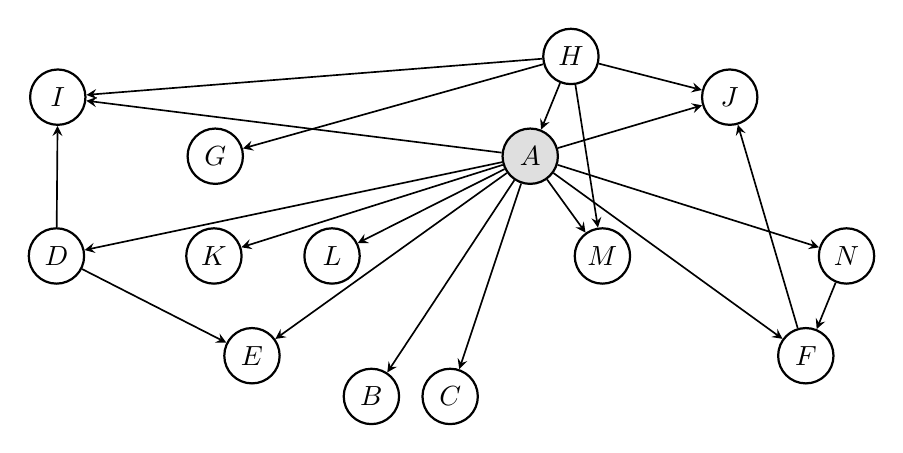
\begin{tikzpicture}[
      nodes={
        draw=black!20, thick, fill=white, font=\normalsize,
        minimum width=2.5em, minimum height=2em
      },
      rounded corners, semithick, >=stealth
      ]

      \node[latent]                 (c8) {$H$};
      \node[obs, below left=0.75 and 0.0 of c8]   (c1){$A$};
      \node[latent, below left=0.75 and 4.0 of c8]   (c7){$G$};
      \node[latent, below right=0.75 and 0.4 of c1] (c13){$M$};
      \node[latent, below right=0.75 and 3.5 of c1] (c14){$N$};
      \node[latent, below left=0.75 and 2.0 of c1] (c12){$L$};
      \node[latent, below left=0.75 and 3.5 of c1] (c11){$K$};
      \node[latent, below left=0.75 and 5.5 of c1] (c4){$D$};
      \node[latent, below left=0.0 and 6.0 of c8] (c9){$I$};
      \node[latent, below left=0.75 and 0.5 of c12] (c5){$E$};
      \node[latent, below left=0.75 and 0.0 of c14] (c6){$F$};
      \node[latent, below right=0.0 and 1.5 of c8] (c10){$J$};
      \node[latent, below right=0.0 and 1.0 of c5] (c2){$B$};   
		\node[latent, below right=0.0 and 2.0 of c5] (c3){$C$};         
      
      %\node[latent, below right = 0.75 and 0.25 of c2] (c5){$5$};
      %\node[latent, below right = 0.75 and 2.0 of c1] (c6) {$6$};
      %\node[latent,below right = 0.75 and 0.5 of c4] (c7){$7$};


  % Connect the nodes
 \edge {c8}{c1,c7,c9,c10,c13};
 \edge {c1}{c4,c11,c12,c2,c3,c14,c13,c9,c10};
 \edge {c1,c4}{c5};
 \edge {c4}{c9};
 \edge {c1,c14}{c6};
 \edge {c6}{c10};
  %\edge {c4}{c7};
  %\draw[->,>=stealth', shorten >= 1pt] (c1) to[bend right](c7);
  %\edge {p1,p2} {y} ; %
  %\edge {y} {c2} ;
  %\edge {y}{c1};



\end{tikzpicture}
%\endpgfgraphicnamed

%%% Local Variables: 
%%% mode: tex-pdf
%%% TeX-master: "example"
%%% End: 
}
  \caption{Structure from prediscretized K2 structure learning to compare the methods for Wine dataset}
  \label{fig:wine_graph_1}
\end{figure}

\begin{table}
  \centering
  \caption{
    Results from discretization of the Wine MPG dataset with fixed structure from Figure~\ref{fig:wine_graph_1}.
    The first thirteen rows list the discretization edges for each continuous variable.
    The last row lists the mean cross-validated log-likelihood; positive values are better.
    The optimal Bayesian approach has the best discretization result in terms of likelihood, but the heuristic method obtains a similar result with nearly the same likelihood.
    The MDL method produces discretization edges for more than half of the continuous variables but does not produce enough discretization intervals.
    Some discretization edges appear in the results of all three methods.
  }
  \scalebox{1.0}{
  \scriptsize
\sisetup{detect-weight = true}
\begin{tabular}{@{}ccc@{}}
\toprule
Variable & Bayesian            & MDL          \\
\midrule
$B$    & \num{12.745}, \num{13.54}                         & \num{12.78}        \\
$C$    & \textbf{\num{1.42}}, \textbf{\num{2.235}}                           & \textbf{\num{1.42}}, \textbf{\num{2.235}}  \\
$D$    & \num{2.03}, \num{2.605}, \num{3.07}               & -            \\
$E$    & \textbf{\num{17.9}}, \num{23.25}                           & \textbf{\num{17.9}}         \\
$F$    & \num{88.5}, \num{135.0}                           & -            \\
$G$    & \num{2.105}, \num{2.58}, \num{3.01}               & -            \\
$H$    & \num{0.975}, \num{1.885}, \num{2.31}, \num{3.355} & -            \\
$I$    & \textbf{\num{0.395}}                                       & \textbf{\num{0.395}}       \\
$J$    & \num{1.185}, \num{1.655}                          & -            \\
$K$    & \textbf{\num{3.46}}, \num{4.85}, \num{7.4}                 & \textbf{\num{3.46}}, \num{7.55}   \\
$L$    & \textbf{\num{0.785}}, \num{1.005}, 1.295                   & \textbf{\num{0.785}}        \\
$M$    & \num{2.475}                                       & \num{2.115}, \num{2.505} \\
$N$    & \num{476.0}, \num{716.0}, \num{900.5}             & -            \\
\addlinespace[0.5em]
Log-Likelihood   & \num{-19.94} & \num{-23.60}        \\
% Logl   & -3550                & -4201        \\
\bottomrule
\end{tabular}
  }
  \label{table:wine_disc_table_1}
\end{table}

Figure~\ref{fig:wine_exp1_distr} compares the optimal Bayesian and MODL discretizaton policies for variables $E$ and $K$ with the original Wine data.
The discretization edges \num{17.9} for $E$ and \num{34.6} for $K$ appear in both plots.
The MDL method does not use enough intervals for discretization.
Relative sensitivities of each method to the input data is discussed in Section~\ref{subsec:discuss_exp}.

\begin{figure}[ht]
  \centering
  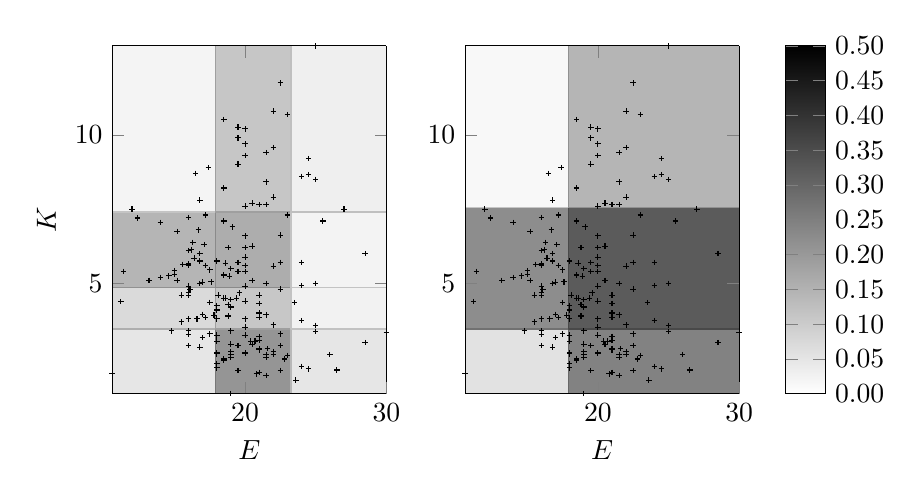
\begin{tikzpicture}
  \begin{groupplot}[
	  	group style={group size=2 by 1,horizontal sep=1cm,
  		}, 
  		width = 1/2*\textwidth - 1cm,
  		height = 6 cm ]%,xmin=0,ymin=0,height=4cm,width=5cm,no markers]
  \nextgroupplot[
			view={0}{90},
			enlargelimits=0,
			zmin=0.0, zmax=1.0,
			ylabel=$K$,
			xlabel=$E$,
			%colorbar,
    %every colorbar/.append style={height=
    %    2*\pgfkeysvalueof{/pgfplots/parent axis height}+
     %   \pgfkeysvalueof{/pgfplots/group/vertical sep}},
		    point meta min=0, point meta max=0.5,
			colormap={}{ gray(0cm)=(1); gray(1cm)=(0);}
			%colorbar style={
			%        ytick={0,0.05,...,0.51},
			%        yticklabel style={
			%            text width=2.5em,
			%            align=right,
			%            /pgf/number format/.cd,
			%                fixed,
			%                fixed zerofill
			%        }
			%    }
			]


			\addplot3[patch,shader=faceted,patch type=rectangle] coordinates {(10.6000,1.2800,0.0495) (17.9000,1.2800,0.0495) (17.9000,3.4600,0.0495) (10.6000,3.4600,0.0495)};
			\addplot3[patch,shader=faceted,patch type=rectangle] coordinates {(10.6000,3.4600,0.0725) (17.9000,3.4600,0.0725) (17.9000,4.8500,0.0725) (10.6000,4.8500,0.0725)};
			\addplot3[patch,shader=faceted,patch type=rectangle] coordinates {(10.6000,4.8500,0.1445) (17.9000,4.8500,0.1445) (17.9000,7.4000,0.1445) (10.6000,7.4000,0.1445)};
			\addplot3[patch,shader=faceted,patch type=rectangle] coordinates {(10.6000,7.4000,0.0205) (17.9000,7.4000,0.0205) (17.9000,13.0000,0.0205) (10.6000,13.0000,0.0205)};

			\addplot3[patch,shader=faceted,patch type=rectangle] coordinates {(17.9000,1.2800,0.2060) (23.2500,1.2800,0.2060) (23.2500,3.4600,0.2060) (17.9000,3.4600,0.2060)};
			\addplot3[patch,shader=faceted,patch type=rectangle] coordinates {(17.9000,3.4600,0.1095) (23.2500,3.4600,0.1095) (23.2500,4.8500,0.1095) (17.9000,4.8500,0.1095)};
			\addplot3[patch,shader=faceted,patch type=rectangle] coordinates {(17.9000,4.8500,0.1600) (23.2500,4.8500,0.1600) (23.2500,7.4000,0.1600) (17.9000,7.4000,0.1600)};
			\addplot3[patch,shader=faceted,patch type=rectangle] coordinates {(17.9000,7.4000,0.1100) (23.2500,7.4000,0.1100) (23.2500,13.0000,0.1100) (17.9000,13.0000,0.1100)};

			\addplot3[patch,shader=faceted,patch type=rectangle] coordinates {(23.2500,1.2800,0.0485) (30.0000,1.2800,0.0485) (30.0000,3.4600,0.0485) (23.2500,3.4600,0.0485)};
			\addplot3[patch,shader=faceted,patch type=rectangle] coordinates {(23.2500,3.4600,0.0255) (30.0000,3.4600,0.0255) (30.0000,4.8500,0.0255) (23.2500,4.8500,0.0255)};
			\addplot3[patch,shader=faceted,patch type=rectangle] coordinates {(23.2500,4.8500,0.0230) (30.0000,4.8500,0.0230) (30.0000,7.4000,0.0230) (23.2500,7.4000,0.0230)};
			\addplot3[patch,shader=faceted,patch type=rectangle] coordinates {(23.2500,7.4000,0.0305) (30.0000,7.4000,0.0305) (30.0000,13.0000,0.0305) (23.2500,13.0000,0.0305)};

			\addplot3[mark=+, draw=none, mark size=1.0] coordinates {
(15.600,5.640,1) (11.200,4.380,1) (18.600,5.680,1) (16.800,7.800,1) (21.000,4.320,1) (15.200,6.750,1) (14.600,5.250,1) (17.600,5.050,1) (14.000,5.200,1) (16.000,7.220,1) (18.000,5.750,1) (16.800,5.000,1) (16.000,5.600,1) (11.400,5.400,1) (12.000,7.500,1) (17.200,7.300,1) (20.000,6.200,1) (20.000,6.600,1) (16.500,8.700,1) (15.200,5.100,1) (16.000,5.650,1) (18.600,4.500,1) (16.600,3.800,1) (17.800,3.930,1) (20.000,3.520,1) (25.000,3.580,1) (16.100,4.800,1) (17.000,3.950,1) (19.400,4.500,1) (16.000,4.700,1) (22.500,5.700,1) (19.100,6.900,1) (17.200,3.840,1) (19.500,5.400,1) (19.000,4.200,1) (20.500,5.100,1) (15.500,4.600,1) (18.000,4.250,1) (15.500,3.700,1) (13.200,5.100,1) (16.200,6.130,1) (18.800,4.280,1) (15.000,5.430,1) (17.500,4.360,1) (17.000,5.040,1) (18.900,5.240,1) (16.000,4.900,1) (16.000,6.100,1) (18.800,6.200,1) (17.400,8.900,1) (12.400,7.200,1) (17.200,5.600,1) (14.000,7.050,1) (17.100,6.300,1) (16.400,5.850,1) (20.500,6.250,1) (16.300,6.380,1) (16.800,6.000,1) (16.700,6.800,1) (10.600,1.950,1) (16.000,3.270,1) (16.800,5.750,1) (18.000,3.800,1) (19.000,4.450,1) (19.000,2.950,1) (18.100,4.600,1) (15.000,5.300,1) (19.600,4.680,1) (17.000,3.170,1) (16.800,2.850,1) (20.400,3.050,1) (25.000,3.380,1) (24.000,3.740,1) (30.000,3.350,1) (21.000,3.210,1) (16.000,3.800,1) (16.000,4.600,1) (18.000,2.650,1) (14.800,3.400,1) (23.000,2.570,1) (19.000,2.500,1) (18.800,3.900,1) (24.000,2.200,1) (22.500,4.800,1) (18.000,3.050,1) (18.000,2.620,1) (22.800,2.450,1) (26.000,2.600,1) (21.600,2.800,1) (23.600,1.740,1) (18.500,2.400,1) (22.000,3.600,1) (20.700,3.050,1) (18.000,2.150,1) (18.000,3.250,1) (19.000,2.600,1) (21.500,2.500,1) (16.000,2.900,1) (18.500,4.500,1) (18.000,2.300,1) (17.500,3.300,1) (18.500,2.450,1) (21.000,2.800,1) (19.500,2.060,1) (20.500,2.940,1) (22.000,2.700,1) (19.000,3.400,1) (22.500,3.300,1) (19.000,2.700,1) (20.000,2.650,1) (19.500,2.900,1) (21.000,2.000,1) (20.000,3.800,1) (21.000,3.080,1) (22.500,2.900,1) (21.500,1.900,1) (20.800,1.950,1) (22.500,2.060,1) (16.000,3.400,1) (19.000,1.280,1) (20.000,3.250,1) (28.500,6.000,1) (26.500,2.080,1) (21.500,2.600,1) (21.000,2.800,1) (21.000,2.760,1) (21.500,3.940,1) (28.500,3.000,1) (24.500,2.120,1) (22.000,2.600,1) (18.000,4.100,1) (20.000,5.400,1) (24.000,5.700,1) (21.500,5.000,1) (17.500,5.450,1) (18.500,7.100,1) (21.000,3.850,1) (25.000,5.000,1) (19.500,5.700,1) (24.000,4.920,1) (21.000,4.600,1) (20.000,5.600,1) (23.500,4.350,1) (20.000,4.400,1) (18.500,8.210,1) (21.000,4.000,1) (20.000,4.900,1) (21.500,7.650,1) (21.500,8.420,1) (21.500,9.400,1) (24.000,8.600,1) (22.000,10.800,1) (25.500,7.100,1) (18.500,10.520,1) (20.000,7.600,1) (22.000,7.900,1) (19.500,9.010,1) (27.000,7.500,1) (25.000,13.000,1) (22.500,11.750,1) (21.000,7.650,1) (20.000,5.880,1) (22.000,5.580,1) (18.500,5.280,1) (22.000,9.580,1) (22.500,6.620,1) (23.000,10.680,1) (19.500,10.260,1) (24.500,8.660,1) (25.000,8.500,1) (19.000,5.500,1) (19.500,9.900,1) (20.000,9.700,1) (20.500,7.700,1) (23.000,7.300,1) (20.000,10.200,1) (20.000,9.300,1) (24.500,9.200,1) };



    \nextgroupplot[
			view={0}{90},
			enlargelimits=0,
			zmin=0.0, zmax=1.0,
			xlabel=$E$,
			%ylabel=K,
			colorbar,
			point meta min=0, point meta max=0.5,
			colormap={}{ gray(0cm)=(1); gray(1cm)=(0);},
			colorbar style={
			        ytick={0,0.05,...,0.51},
			        yticklabel style={
			            text width=1.5em,
			            align=right,
			           /pgf/number format/.cd,
			                fixed,
			                fixed zerofill
			        }
			    }
			]

    		\addplot3[patch,shader=faceted,patch type=rectangle] coordinates {(10.6000,1.2800,0.0565) (17.9000,1.2800,0.0565) (17.9000,3.4600,0.0565) (10.6000,3.4600,0.0565)};
			\addplot3[patch,shader=faceted,patch type=rectangle] coordinates {(10.6000,3.4600,0.2210) (17.9000,3.4600,0.2210) (17.9000,7.5500,0.2210) (10.6000,7.5500,0.2210)};
			\addplot3[patch,shader=faceted,patch type=rectangle] coordinates {(10.6000,7.5500,0.0145) (17.9000,7.5500,0.0145) (17.9000,13.0000,0.0145) (10.6000,13.0000,0.0145)};

			\addplot3[patch,shader=faceted,patch type=rectangle] coordinates {(17.9000,1.2800,0.2440) (30.0000,1.2800,0.2440) (30.0000,3.4600,0.2440) (17.9000,3.4600,0.2440)};
			\addplot3[patch,shader=faceted,patch type=rectangle] coordinates {(17.9000,3.4600,0.3195) (30.0000,3.4600,0.3195) (30.0000,7.5500,0.3195) (17.9000,7.5500,0.3195)};
			\addplot3[patch,shader=faceted,patch type=rectangle] coordinates {(17.9000,7.5500,0.1445) (30.0000,7.5500,0.1445) (30.0000,13.0000,0.1445) (17.9000,13.0000,0.1445)};

			\addplot3[mark=+, draw=none, mark size=1.0] coordinates {
(15.600,5.640,1) (11.200,4.380,1) (18.600,5.680,1) (16.800,7.800,1) (21.000,4.320,1) (15.200,6.750,1) (14.600,5.250,1) (17.600,5.050,1) (14.000,5.200,1) (16.000,7.220,1) (18.000,5.750,1) (16.800,5.000,1) (16.000,5.600,1) (11.400,5.400,1) (12.000,7.500,1) (17.200,7.300,1) (20.000,6.200,1) (20.000,6.600,1) (16.500,8.700,1) (15.200,5.100,1) (16.000,5.650,1) (18.600,4.500,1) (16.600,3.800,1) (17.800,3.930,1) (20.000,3.520,1) (25.000,3.580,1) (16.100,4.800,1) (17.000,3.950,1) (19.400,4.500,1) (16.000,4.700,1) (22.500,5.700,1) (19.100,6.900,1) (17.200,3.840,1) (19.500,5.400,1) (19.000,4.200,1) (20.500,5.100,1) (15.500,4.600,1) (18.000,4.250,1) (15.500,3.700,1) (13.200,5.100,1) (16.200,6.130,1) (18.800,4.280,1) (15.000,5.430,1) (17.500,4.360,1) (17.000,5.040,1) (18.900,5.240,1) (16.000,4.900,1) (16.000,6.100,1) (18.800,6.200,1) (17.400,8.900,1) (12.400,7.200,1) (17.200,5.600,1) (14.000,7.050,1) (17.100,6.300,1) (16.400,5.850,1) (20.500,6.250,1) (16.300,6.380,1) (16.800,6.000,1) (16.700,6.800,1) (10.600,1.950,1) (16.000,3.270,1) (16.800,5.750,1) (18.000,3.800,1) (19.000,4.450,1) (19.000,2.950,1) (18.100,4.600,1) (15.000,5.300,1) (19.600,4.680,1) (17.000,3.170,1) (16.800,2.850,1) (20.400,3.050,1) (25.000,3.380,1) (24.000,3.740,1) (30.000,3.350,1) (21.000,3.210,1) (16.000,3.800,1) (16.000,4.600,1) (18.000,2.650,1) (14.800,3.400,1) (23.000,2.570,1) (19.000,2.500,1) (18.800,3.900,1) (24.000,2.200,1) (22.500,4.800,1) (18.000,3.050,1) (18.000,2.620,1) (22.800,2.450,1) (26.000,2.600,1) (21.600,2.800,1) (23.600,1.740,1) (18.500,2.400,1) (22.000,3.600,1) (20.700,3.050,1) (18.000,2.150,1) (18.000,3.250,1) (19.000,2.600,1) (21.500,2.500,1) (16.000,2.900,1) (18.500,4.500,1) (18.000,2.300,1) (17.500,3.300,1) (18.500,2.450,1) (21.000,2.800,1) (19.500,2.060,1) (20.500,2.940,1) (22.000,2.700,1) (19.000,3.400,1) (22.500,3.300,1) (19.000,2.700,1) (20.000,2.650,1) (19.500,2.900,1) (21.000,2.000,1) (20.000,3.800,1) (21.000,3.080,1) (22.500,2.900,1) (21.500,1.900,1) (20.800,1.950,1) (22.500,2.060,1) (16.000,3.400,1) (19.000,1.280,1) (20.000,3.250,1) (28.500,6.000,1) (26.500,2.080,1) (21.500,2.600,1) (21.000,2.800,1) (21.000,2.760,1) (21.500,3.940,1) (28.500,3.000,1) (24.500,2.120,1) (22.000,2.600,1) (18.000,4.100,1) (20.000,5.400,1) (24.000,5.700,1) (21.500,5.000,1) (17.500,5.450,1) (18.500,7.100,1) (21.000,3.850,1) (25.000,5.000,1) (19.500,5.700,1) (24.000,4.920,1) (21.000,4.600,1) (20.000,5.600,1) (23.500,4.350,1) (20.000,4.400,1) (18.500,8.210,1) (21.000,4.000,1) (20.000,4.900,1) (21.500,7.650,1) (21.500,8.420,1) (21.500,9.400,1) (24.000,8.600,1) (22.000,10.800,1) (25.500,7.100,1) (18.500,10.520,1) (20.000,7.600,1) (22.000,7.900,1) (19.500,9.010,1) (27.000,7.500,1) (25.000,13.000,1) (22.500,11.750,1) (21.000,7.650,1) (20.000,5.880,1) (22.000,5.580,1) (18.500,5.280,1) (22.000,9.580,1) (22.500,6.620,1) (23.000,10.680,1) (19.500,10.260,1) (24.500,8.660,1) (25.000,8.500,1) (19.000,5.500,1) (19.500,9.900,1) (20.000,9.700,1) (20.500,7.700,1) (23.000,7.300,1) (20.000,10.200,1) (20.000,9.300,1) (24.500,9.200,1) };
  \end{groupplot}
\end{tikzpicture}
  \caption{Comparison of the discretization policies for variables $A$ and $C$ obtained using optimal Bayesian and MDL methods}
  \label{fig:wine_exp1_distr}
\end{figure}

\subsubsection{Discretization while Learning Structure}
\label{subsubsec:wine_exp2}

Figure~\ref{fig:wine_graph_2} is the discrete-valued Bayesian network learned from the Wine dataset, obtained by running Algorithm~\ref{alg:structure_learn} fifty times.
A comparison of Figures~\ref{fig:wine_graph_2} and \ref{fig:wine_graph_1} show that the Bayesian network learned during the discretization process has more edges than the network learned on the prediscretized data.
When a network is learned along with discretization, the algorithm has more freedom to adjust the structure and the discretization policy simultaneously to identify useful correlations and produce a denser structure.

Figure~\ref{fig:wine_exp2_distr} shows the discretization policy for variables $E$ and $K$ obtained with the optimal Bayesian method.
The discretization edge $E = 17.9$ also appears in all discretization policies from the fixed network (Figure~\ref{fig:wine_exp1_distr}).
This indicates that some discretization edges are robust against the network structure.
Furthermore, the discretization edge at $E = 23.5$ present in the fixed-structure case is missing in the learned structure.
This is caused by $E$ having twice as many parents in the learned network structure.
The more parents a variable has, the less discretization intervals it will be able to support, as the set of statistics required to define the resulting distribution increases exponentially with the number of parents.

\begin{figure}[ht]
  \centering
  \scalebox{0.7}{% model_pca.tex
%
% Copyright (C) 2012 Jaakko Luttinen
%
% This file may be distributed and/or modified
%
% 1. under the LaTeX Project Public License and/or
% 2. under the GNU General Public License.
%
% See the files LICENSE_LPPL and LICENSE_GPL for more details.

% PCA model

%\beginpgfgraphicnamed{model-pca}
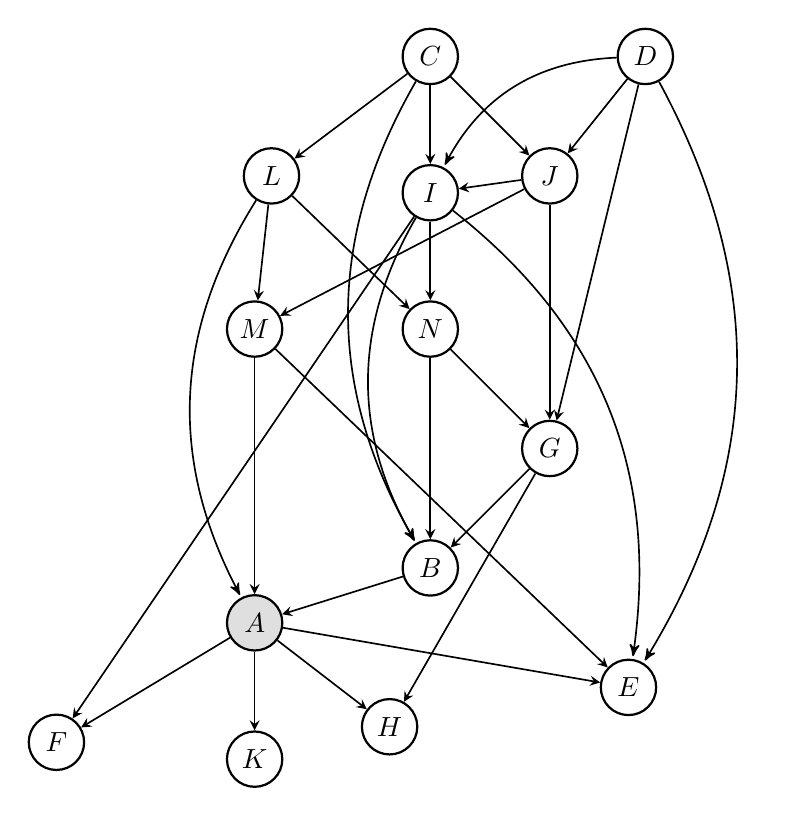
\begin{tikzpicture}[
      nodes={
        draw=black!20, thick, fill=white, font=\normalsize,
        minimum width=2.5em, minimum height=2em
      },
      rounded corners, semithick, >=stealth
      ]

	  \node[latent]          (c3) {$C$};
	  \node[latent, right = 2.0 of c3]  (c4){$D$};
	  \node[latent, below right = 1.0 and 1.0 of c3]  (c10){$J$};
	  \node[latent, below = 1.0 of c3]  (c9){$I$};
	  \node[latent, below = 1.0 of c9]  (c14){$N$};
	  \node[latent, below right = 1.0 and 1.0 of c14] (c7){$G$};
	  \node[latent, below left = 1.0 and 1.0 of c7]  (c2){$B$};
	  \node[latent, below right = 1.0 and 2.0 of c2] (c5){$E$};
	  \node[latent, below left = 1.5 and 0.0 of c2] (c8){$H$};
	  \node[latent, below left = 1.0 and 1.5 of c3] (c12){$L$};
	  \node[latent, left = 1.5 of c14] (c13){$M$};
	  \node[obs, below = 3.0 of c13] (c1){$A$};
	  \node[latent, below = 1.0 of c1] (c11){$K$};
	  \node[latent, below left = 1.0 and 2.0 of c1] (c6){$F$};


  % Connect the nodes

  \edge {c3}{c12,c10,c9};
  \draw[->,>=stealth', shorten >= 1pt] (c3) to[bend right](c2);
  \edge {c4}{c10,c7}
  \draw[->,>=stealth', shorten >= 1pt] (c4) to[bend right](c9);
  \draw[->,>=stealth', shorten >= 1pt] (c4) to[bend left](c5);  
  \edge {c10}{c9,c7,c13};
  \edge{c9}{c14,c6};
  \draw[->,>=stealth', shorten >= 1pt] (c9) to[bend left](c5);
  \draw[->,>=stealth', shorten >= 1pt] (c9) to[bend right](c2);
  \edge {c14}{c2,c7};
  \edge {c7}{c2,c8};
  \edge {c12}{c13,c14};
  \edge {c13}{c1,c5};
  \edge {c1}{c6,c11,c8,c5};
  \edge {c2}{c1};
  \draw[->,>=stealth', shorten >= 1pt] (c12) to[bend right](c1);
  %\draw[->,>=stealth', shorten >= 1pt] (c1) to[bend right](c7);
  %\edge {p1,p2} {y} ; %
  %\edge {y} {c2} ;
  %\edge {y}{c1};



\end{tikzpicture}
%\endpgfgraphicnamed

%%% Local Variables: 
%%% mode: tex-pdf
%%% TeX-master: "example"
%%% End: 
}
  \caption{The discrete-valued Bayesian network learned from the Wine dataset using the optimal Bayesian method.}
  \label{fig:wine_graph_2}
\end{figure}

\begin{figure}[ht]
  \centering
  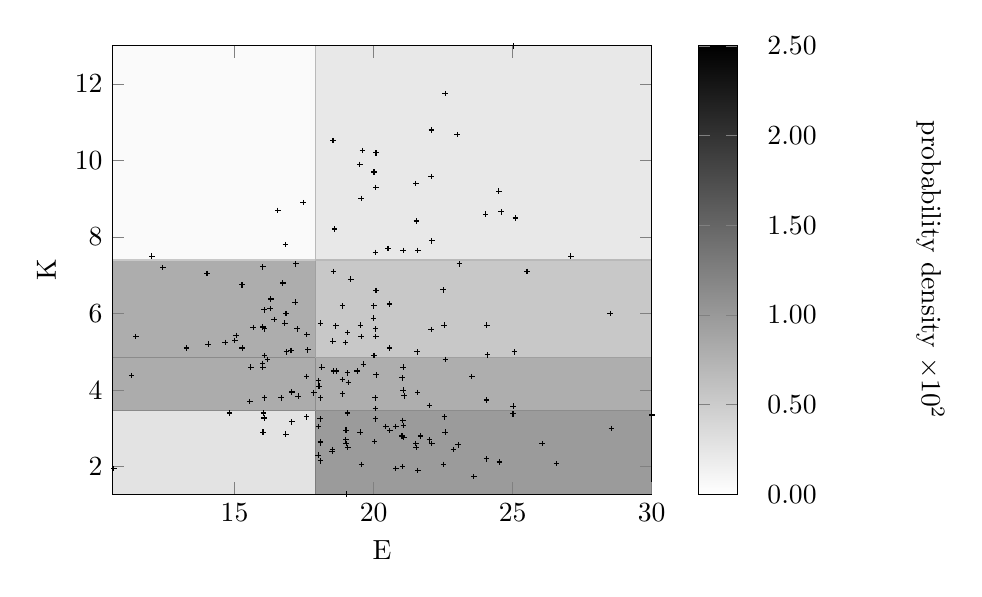
\begin{tikzpicture}
		\begin{axis}[
			view={0}{90},
			enlargelimits=0,
			zmin=0.0, zmax=1.0,
			xlabel=E,
			ylabel=K,
			colorbar,
			point meta min=0, point meta max=2.5,
			colormap={}{ gray(0cm)=(1); gray(1cm)=(0);},
			colorbar style={
			        ytick={0,0.5,...,2.6},
			        ylabel={probability density $\times 10^2$},
			        y label style={at={(axis description cs:6.5,0.5)},rotate=180,anchor=north},
			        yticklabel style={
			            text width=2.5em,
			            align=right,
			            /pgf/number format/.cd,
			                fixed,
			                fixed zerofill
			        }
			    }
			]

			\addplot3[patch,shader=faceted,patch type=rectangle] coordinates {(10.6000,1.2800,0.276486) (17.9000,1.2800,0.276486) (17.9000,3.4600,0.2765) (10.6000,3.4600,0.2765)};
			\addplot3[patch,shader=faceted,patch type=rectangle] coordinates {(10.6000,3.4600,0.808121) (17.9000,3.4600,0.808121) (17.9000,4.8500,0.8081) (10.6000,4.8500,0.8081)};
			\addplot3[patch,shader=faceted,patch type=rectangle] coordinates {(10.6000,4.8500,0.795058) (17.9000,4.8500,0.795058) (17.9000,7.4000,0.7951) (10.6000,7.4000,0.7951)};
			\addplot3[patch,shader=faceted,patch type=rectangle] coordinates {(10.6000,7.4000,0.047701) (17.9000,7.4000,0.047701) (17.9000,13.0000,0.0477) (10.6000,13.0000,0.0477)};

			\addplot3[patch,shader=faceted,patch type=rectangle] coordinates {(17.9000,1.2800,0.972401) (30.0000,1.2800,0.972401) (30.0000,3.4600,0.9724) (17.9000,3.4600,0.9724)};
			\addplot3[patch,shader=faceted,patch type=rectangle] coordinates {(17.9000,3.4600,0.784827) (30.0000,3.4600,0.784827) (30.0000,4.8500,0.7848) (17.9000,4.8500,0.7848)};
			\addplot3[patch,shader=faceted,patch type=rectangle] coordinates {(17.9000,4.8500,0.531518) (30.0000,4.8500,0.531518) (30.0000,7.4000,0.5315) (17.9000,7.4000,0.5315)};
			\addplot3[patch,shader=faceted,patch type=rectangle] coordinates {(17.9000,7.4000,0.227273) (30.0000,7.4000,0.227273) (30.0000,13.0000,0.2273) (17.9000,13.0000,0.2273)};

			\addplot3[mark=+, draw=none, mark size=1.0, jitter = 0.1] coordinates {
(15.600,5.640,1) (11.200,4.380,1) (18.600,5.680,1) (16.800,7.800,1) (21.000,4.320,1) (15.200,6.750,1) (14.600,5.250,1) (17.600,5.050,1) (14.000,5.200,1) (16.000,7.220,1) (18.000,5.750,1) (16.800,5.000,1) (16.000,5.600,1) (11.400,5.400,1) (12.000,7.500,1) (17.200,7.300,1) (20.000,6.200,1) (20.000,6.600,1) (16.500,8.700,1) (15.200,5.100,1) (16.000,5.650,1) (18.600,4.500,1) (16.600,3.800,1) (17.800,3.930,1) (20.000,3.520,1) (25.000,3.580,1) (16.100,4.800,1) (17.000,3.950,1) (19.400,4.500,1) (16.000,4.700,1) (22.500,5.700,1) (19.100,6.900,1) (17.200,3.840,1) (19.500,5.400,1) (19.000,4.200,1) (20.500,5.100,1) (15.500,4.600,1) (18.000,4.250,1) (15.500,3.700,1) (13.200,5.100,1) (16.200,6.130,1) (18.800,4.280,1) (15.000,5.430,1) (17.500,4.360,1) (17.000,5.040,1) (18.900,5.240,1) (16.000,4.900,1) (16.000,6.100,1) (18.800,6.200,1) (17.400,8.900,1) (12.400,7.200,1) (17.200,5.600,1) (14.000,7.050,1) (17.100,6.300,1) (16.400,5.850,1) (20.500,6.250,1) (16.300,6.380,1) (16.800,6.000,1) (16.700,6.800,1) (10.600,1.950,1) (16.000,3.270,1) (16.800,5.750,1) (18.000,3.800,1) (19.000,4.450,1) (19.000,2.950,1) (18.100,4.600,1) (15.000,5.300,1) (19.600,4.680,1) (17.000,3.170,1) (16.800,2.850,1) (20.400,3.050,1) (25.000,3.380,1) (24.000,3.740,1) (30.000,3.350,1) (21.000,3.210,1) (16.000,3.800,1) (16.000,4.600,1) (18.000,2.650,1) (14.800,3.400,1) (23.000,2.570,1) (19.000,2.500,1) (18.800,3.900,1) (24.000,2.200,1) (22.500,4.800,1) (18.000,3.050,1) (18.000,2.620,1) (22.800,2.450,1) (26.000,2.600,1) (21.600,2.800,1) (23.600,1.740,1) (18.500,2.400,1) (22.000,3.600,1) (20.700,3.050,1) (18.000,2.150,1) (18.000,3.250,1) (19.000,2.600,1) (21.500,2.500,1) (16.000,2.900,1) (18.500,4.500,1) (18.000,2.300,1) (17.500,3.300,1) (18.500,2.450,1) (21.000,2.800,1) (19.500,2.060,1) (20.500,2.940,1) (22.000,2.700,1) (19.000,3.400,1) (22.500,3.300,1) (19.000,2.700,1) (20.000,2.650,1) (19.500,2.900,1) (21.000,2.000,1) (20.000,3.800,1) (21.000,3.080,1) (22.500,2.900,1) (21.500,1.900,1) (20.800,1.950,1) (22.500,2.060,1) (16.000,3.400,1) (19.000,1.280,1) (20.000,3.250,1) (28.500,6.000,1) (26.500,2.080,1) (21.500,2.600,1) (21.000,2.800,1) (21.000,2.760,1) (21.500,3.940,1) (28.500,3.000,1) (24.500,2.120,1) (22.000,2.600,1) (18.000,4.100,1) (20.000,5.400,1) (24.000,5.700,1) (21.500,5.000,1) (17.500,5.450,1) (18.500,7.100,1) (21.000,3.850,1) (25.000,5.000,1) (19.500,5.700,1) (24.000,4.920,1) (21.000,4.600,1) (20.000,5.600,1) (23.500,4.350,1) (20.000,4.400,1) (18.500,8.210,1) (21.000,4.000,1) (20.000,4.900,1) (21.500,7.650,1) (21.500,8.420,1) (21.500,9.400,1) (24.000,8.600,1) (22.000,10.800,1) (25.500,7.100,1) (18.500,10.520,1) (20.000,7.600,1) (22.000,7.900,1) (19.500,9.010,1) (27.000,7.500,1) (25.000,13.000,1) (22.500,11.750,1) (21.000,7.650,1) (20.000,5.880,1) (22.000,5.580,1) (18.500,5.280,1) (22.000,9.580,1) (22.500,6.620,1) (23.000,10.680,1) (19.500,10.260,1) (24.500,8.660,1) (25.000,8.500,1) (19.000,5.500,1) (19.500,9.900,1) (20.000,9.700,1) (20.500,7.700,1) (23.000,7.300,1) (20.000,10.200,1) (20.000,9.300,1) (24.500,9.200,1) };
		\end{axis}
	\end{tikzpicture}

  \caption{
    The discretization policy for variables $E$ and $K$ on the learned network in Figure~\ref{fig:wine_graph_2}.
    The discretization edge $E = 17.9$ also appears in the policies for the fixed network.
    This indicates that some discretization edges are robust against changing network structure.
  }
  \label{fig:wine_exp2_distr}
\end{figure}

%%%%%%%%%%%%%%%%%%%%%%%%%%%%%%%%%%%%%%%%%%
%
% Housing
%
%%%%%%%%%%%%%%%%%%%%%%%%%%%%%%%%%%%%%%%%%%

\subsection{Data 3: Housing}
\label{subsec:housing}

The Housing dataset contains variables related to the values of houses in Boston suburbs.
The dataset has \num{506} samples over fourteen variables.
Only variables $D$ and $I$ are discrete-valued, with \num{2} and \num{9} instantiations, respectively.
Variable $A$ is the only discrete variable and has three instantiations.
Despite their being continuous, several variables in the Housing dataset possess many repeated values.
The following experiments were conducted with an upper limit of three on the number of parents per variable to prevent memory issues with MDL.

\subsubsection{Discretization with Fixed Structure}
\label{subsubsec:housing_exp1}

The Bayesian network structure in Figure~\ref{fig:housing_graph_1} was obtained by prediscretizing each continuous variable into five uniform-width interval and then running the K2 algorithm one thousand times and choosing the network with the highest likelihood.
Table~\ref{table:housing_disc_table_1} shows the numbers of intervals after discretization for each continuous variables and the log-likelihood of the dataset based on each discretization method.
MDL method does not produce any discretization edges for most variables.
The heuristic Bayesian method produces far more discretization edges than the optimal Bayesian method due to repeated instances in the dataset.
These numbers of intervals returned by the three methods illustrate the over-sensitive nature of the heuristic method and the under-sensitive nature of the MDL method.
\tim{I am not sure we are using `sensitive' correctly. Sensitive to what? Perhaps `biased towards higher edge counts'?}
The relative sensitivity of each algorithm will be discussed in Section~\ref{subsec:discuss_exp}.

The heurstic method produces the discretization with the highest cross-validated log likelihood, but although the heuristic method leads to a higher number of intervals, its likelihood is not significantly better than the optimal Bayesian approach.
This shows that the optimal Bayesian approach captures the most important discretization edges.

\begin{figure}[ht]
  \centering
  \scalebox{0.8}{% model_pca.tex
%
% Copyright (C) 2012 Jaakko Luttinen
%
% This file may be distributed and/or modified
%
% 1. under the LaTeX Project Public License and/or
% 2. under the GNU General Public License.
%
% See the files LICENSE_LPPL and LICENSE_GPL for more details.

% PCA model

%\beginpgfgraphicnamed{model-pca}
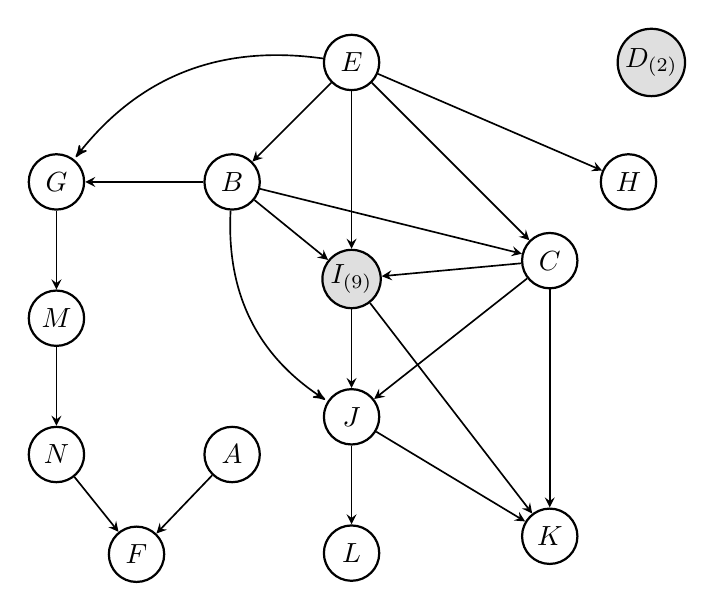
\begin{tikzpicture}[
      nodes={
        draw=black!20, thick, fill=white, font=\normalsize,
        minimum width=2.5em, minimum height=2em
      },
      rounded corners, semithick, >=stealth
      ]

	  \node[latent]          (c5) {$E$};
	  \node[obs, right = 3.0 of c5]  (c4){$D_{{(2)}}$};
	  \node[latent, below left = 1.0 and 1.0 of c5]  (c2){$B$};
	  \node[obs, below = 2.0 of c5]  (c9){$I_{{(9)}}$};
	  \node[latent, below = 1.0 of c9]  (c10){$J$};
	  \node[latent, below = 1.0 of c10] (c12){$L$};
	  \node[latent, below right = 1.0 and 2.0 of c10]  (c11){$K$};
	  \node[latent, below right = 2.0 and 2.0 of c5] (c3){$C$};
	  \node[latent, below right = 1.0 and 3.0 of c5] (c8){$H$};
	  \node[latent, left = 1.5 of c2] (c7){$G$};
	  \node[latent, below = 1.0 of c7] (c13){$M$};
	  \node[latent, below = 1.0 of c13] (c14){$N$};
	  \node[latent, right = 1.5 of c14] (c1){$A$};
	  \node[latent, below right = 0.75 and 0.5 of c14] (c6){$F$};


  % Connect the nodes

  \edge {c5}{c2,c3,c8,c9};
  \draw[->,>=stealth', shorten >= 1pt] (c5) to[bend right](c7);
  \edge {c2}{c9,c3,c7}
  \draw[->,>=stealth', shorten >= 1pt] (c2) to[bend right](c10);
  %\draw[->,>=stealth', shorten >= 1pt] (c4) to[bend left](c5);  
  \edge {c3}{c9,c10,c11};
  \edge{c9}{c10,c11};
  %\draw[->,>=stealth', shorten >= 1pt] (c9) to[bend left](c5);
  %\draw[->,>=stealth', shorten >= 1pt] (c9) to[bend right](c2);
  \edge {c10}{c11,c12};
  \edge {c7}{c13};
  \edge {c13}{c14};
  \edge {c14,c1}{c6};
  %\edge {c1}{c6,c11,c8,c5};
  %\edge {c2}{c1};
  %\draw[->,>=stealth', shorten >= 1pt] (c12) to[bend right](c1);
  %\draw[->,>=stealth', shorten >= 1pt] (c1) to[bend right](c7);
  %\edge {p1,p2} {y} ; %
  %\edge {y} {c2} ;
  %\edge {y}{c1};



\end{tikzpicture}
%\endpgfgraphicnamed

%%% Local Variables: 
%%% mode: tex-pdf
%%% TeX-master: "example"
%%% End: 
}
  \caption{Structure from prediscretized K2 structure learning to compare the methods for Housing dataset}
  \label{fig:housing_graph_1}
\end{figure}

\begin{table}
  \centering
  \caption{
    Discretization policy summary of the Housing dataset based on the fixed network structure shown in Figure~\ref{fig:housing_graph_1}.
    The first twelve rows show the numbers of intervals after discretization by each method.
    The last row is the mean cross-validated log-likelihood of the dataset based on the discretization results.
    The heuristic method is over-sensitive \todo{to what?} and discretizes some variables into too many intervals.
    The MDL method is less sensitive and on many cases does not produce any discretization intervals.
    The optimal Bayesian approach produces a reasonable number of discretization edges.
  }
  \scalebox{1.0}{\begin{tabular}{|c|c|c|c|}
\hline
                                                              & The Proposed Method                                     & \begin{tabular}[c]{@{}c@{}}The Proposed Method\\ With the Approx.\end{tabular} & \begin{tabular}[c]{@{}c@{}}The MDL\\ Discretization\end{tabular} \\ \hline
\begin{tabular}[c]{@{}c@{}}Continuous\\ Variable\end{tabular} & \begin{tabular}[c]{@{}c@{}}No. of\\ Intvls\end{tabular} & \begin{tabular}[c]{@{}c@{}}No. of\\ Intvls\end{tabular}                        & \begin{tabular}[c]{@{}c@{}}No. of\\ Intvls\end{tabular}          \\ \hline
$A$                                                             & 3                                                       & 8                                                                              & 1                                                                \\ \hline
$B$                                                             & 4                                                       & 6                                                                              & 1                                                                \\ \hline
$C$                                                             & 8                                                       & 40                                                                             & 1                                                                \\ \hline
$E$                                                             & 14                                                      & 15                                                                             & 1                                                                \\ \hline
$F$                                                             & 4                                                       & 9                                                                              & 1                                                                \\ \hline
$G$                                                             & 3                                                       & 5                                                                              & 1                                                                \\ \hline
$H$                                                             & 6                                                       & 10                                                                             & 1                                                                \\ \hline
$J$                                                            & 8                                                       & 58                                                                             & 1                                                                \\ \hline
$K$                                                             & 5                                                       & 46                                                                             & 7                                                                \\ \hline
$L$                                                             & 4                                                       & 3                                                                              & 1                                                                \\ \hline
$M$                                                             & 6                                                       & 5                                                                              & 1                                                                \\ \hline
$N$                                                             & 6                                                       & 5                                                                              & 1                                                                \\ \hline
\begin{tabular}[c]{@{}c@{}}log-\\ likelihood\end{tabular}     &  -15886.6364                                            & -14559.4739                                                                    & -2186.4531                                                       \\ \hline
\end{tabular}}
  \label{table:housing_disc_table_1}
\end{table}

Figures~\ref{fig:housing_exp1_distr_3_5} and \ref{fig:housing_exp1_distr_8_5} show the discretization policy learned using the optimal Bayesian approach on the fixed network shown in Figure~\ref{fig:housing_graph_1}.
In Figure~\ref{fig:housing_exp1_distr_3_5}, the scatter points corresponding to the original dataset have been jittered, because there are many repeated values for variables $C$ and $E$.
Each repeated point forms a single discrete region, thereby encouraging discretization.
In contrast, the samples for $H$ are well spread out, resulting in fewer discretization regions and larger discretization intervals.

\begin{figure}[ht]
  \centering
  	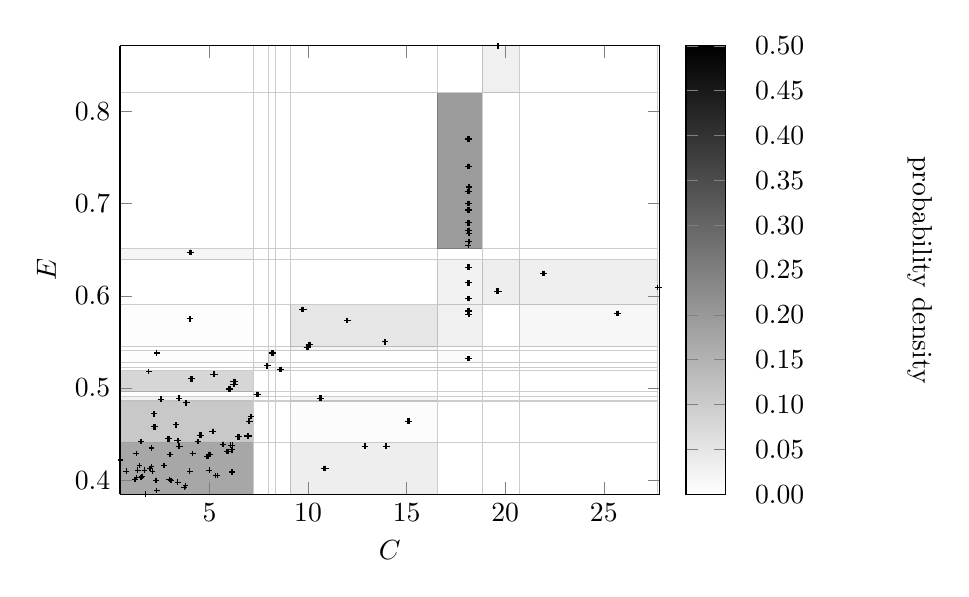
\begin{tikzpicture}
		\begin{axis}[
			view={0}{90},
			enlargelimits=0,
			zmin=0.0, zmax=1.0,
			xlabel=$C$,
			ylabel=$E$,
			colorbar,
			point meta min=0, point meta max=0.50,
			colormap={}{ gray(0cm)=(1); gray(1cm)=(0);},
			colorbar style={
			        ytick={0,0.05,...,0.51},
			        ylabel=probability density,
			        y label style={at={(axis description cs:6.5,0.5)},rotate=180,anchor=north},
			        yticklabel style={
			            text width=2.5em,
			            align=right,
			            /pgf/number format/.cd,
			                fixed,
			                fixed zerofill
			        }
			    }
			]

			\addplot3[patch,shader=faceted,patch type=rectangle] coordinates {(0.4600,0.3850,0.1710) (7.2250,0.3850,0.1710) (7.2250,0.4405,0.1710) (0.4600,0.4405,0.1710)};
			\addplot3[patch,shader=faceted,patch type=rectangle] coordinates {(0.4600,0.4405,0.1080) (7.2250,0.4405,0.1080) (7.2250,0.4860,0.1080) (0.4600,0.4860,0.1080)};
			\addplot3[patch,shader=faceted,patch type=rectangle] coordinates {(0.4600,0.4860,0.0250) (7.2250,0.4860,0.0250) (7.2250,0.4910,0.0250) (0.4600,0.4910,0.0250)};
			\addplot3[patch,shader=faceted,patch type=rectangle] coordinates {(0.4600,0.4910,0.0000) (7.2250,0.4910,0.0000) (7.2250,0.4960,0.0000) (0.4600,0.4960,0.0000)};
			\addplot3[patch,shader=faceted,patch type=rectangle] coordinates {(0.4600,0.4960,0.0795) (7.2250,0.4960,0.0795) (7.2250,0.5190,0.0795) (0.4600,0.5190,0.0795)};
			\addplot3[patch,shader=faceted,patch type=rectangle] coordinates {(0.4600,0.5190,0.0000) (7.2250,0.5190,0.0000) (7.2250,0.5220,0.0000) (0.4600,0.5220,0.0000)};
			\addplot3[patch,shader=faceted,patch type=rectangle] coordinates {(0.4600,0.5220,0.0000) (7.2250,0.5220,0.0000) (7.2250,0.5280,0.0000) (0.4600,0.5280,0.0000)};
			\addplot3[patch,shader=faceted,patch type=rectangle] coordinates {(0.4600,0.5280,0.0035) (7.2250,0.5280,0.0035) (7.2250,0.5410,0.0035) (0.4600,0.5410,0.0035)};
			\addplot3[patch,shader=faceted,patch type=rectangle] coordinates {(0.4600,0.5410,0.0000) (7.2250,0.5410,0.0000) (7.2250,0.5455,0.0000) (0.4600,0.5455,0.0000)};
			\addplot3[patch,shader=faceted,patch type=rectangle] coordinates {(0.4600,0.5455,0.0045) (7.2250,0.5455,0.0045) (7.2250,0.5910,0.0045) (0.4600,0.5910,0.0045)};
			\addplot3[patch,shader=faceted,patch type=rectangle] coordinates {(0.4600,0.5910,0.0000) (7.2250,0.5910,0.0000) (7.2250,0.6390,0.0000) (0.4600,0.6390,0.0000)};
			\addplot3[patch,shader=faceted,patch type=rectangle] coordinates {(0.4600,0.6390,0.0185) (7.2250,0.6390,0.0185) (7.2250,0.6510,0.0185) (0.4600,0.6510,0.0185)};
			\addplot3[patch,shader=faceted,patch type=rectangle] coordinates {(0.4600,0.6510,0.0000) (7.2250,0.6510,0.0000) (7.2250,0.8205,0.0000) (0.4600,0.8205,0.0000)};
			\addplot3[patch,shader=faceted,patch type=rectangle] coordinates {(0.4600,0.8205,0.0000) (7.2250,0.8205,0.0000) (7.2250,0.8710,0.0000) (0.4600,0.8710,0.0000)};

			\addplot3[patch,shader=faceted,patch type=rectangle] coordinates {(7.2250,0.3850,0.0000) (8.0050,0.3850,0.0000) (8.0050,0.4405,0.0000) (7.2250,0.4405,0.0000)};
			\addplot3[patch,shader=faceted,patch type=rectangle] coordinates {(7.2250,0.4405,0.0000) (8.0050,0.4405,0.0000) (8.0050,0.4860,0.0000) (7.2250,0.4860,0.0000)};
			\addplot3[patch,shader=faceted,patch type=rectangle] coordinates {(7.2250,0.4860,0.0000) (8.0050,0.4860,0.0000) (8.0050,0.4910,0.0000) (7.2250,0.4910,0.0000)};
			\addplot3[patch,shader=faceted,patch type=rectangle] coordinates {(7.2250,0.4910,0.0145) (8.0050,0.4910,0.0145) (8.0050,0.4960,0.0145) (7.2250,0.4960,0.0145)};
			\addplot3[patch,shader=faceted,patch type=rectangle] coordinates {(7.2250,0.4960,0.0000) (8.0050,0.4960,0.0000) (8.0050,0.5190,0.0000) (7.2250,0.5190,0.0000)};
			\addplot3[patch,shader=faceted,patch type=rectangle] coordinates {(7.2250,0.5190,0.0000) (8.0050,0.5190,0.0000) (8.0050,0.5220,0.0000) (7.2250,0.5220,0.0000)};
			\addplot3[patch,shader=faceted,patch type=rectangle] coordinates {(7.2250,0.5220,0.0120) (8.0050,0.5220,0.0120) (8.0050,0.5280,0.0120) (7.2250,0.5280,0.0120)};
			\addplot3[patch,shader=faceted,patch type=rectangle] coordinates {(7.2250,0.5280,0.0000) (8.0050,0.5280,0.0000) (8.0050,0.5410,0.0000) (7.2250,0.5410,0.0000)};
			\addplot3[patch,shader=faceted,patch type=rectangle] coordinates {(7.2250,0.5410,0.0000) (8.0050,0.5410,0.0000) (8.0050,0.5455,0.0000) (7.2250,0.5455,0.0000)};
			\addplot3[patch,shader=faceted,patch type=rectangle] coordinates {(7.2250,0.5455,0.0000) (8.0050,0.5455,0.0000) (8.0050,0.5910,0.0000) (7.2250,0.5910,0.0000)};
			\addplot3[patch,shader=faceted,patch type=rectangle] coordinates {(7.2250,0.5910,0.0000) (8.0050,0.5910,0.0000) (8.0050,0.6390,0.0000) (7.2250,0.6390,0.0000)};
			\addplot3[patch,shader=faceted,patch type=rectangle] coordinates {(7.2250,0.6390,0.0000) (8.0050,0.6390,0.0000) (8.0050,0.6510,0.0000) (7.2250,0.6510,0.0000)};
			\addplot3[patch,shader=faceted,patch type=rectangle] coordinates {(7.2250,0.6510,0.0000) (8.0050,0.6510,0.0000) (8.0050,0.8205,0.0000) (7.2250,0.8205,0.0000)};
			\addplot3[patch,shader=faceted,patch type=rectangle] coordinates {(7.2250,0.8205,0.0000) (8.0050,0.8205,0.0000) (8.0050,0.8710,0.0000) (7.2250,0.8710,0.0000)};

			\addplot3[patch,shader=faceted,patch type=rectangle] coordinates {(8.0050,0.3850,0.0000) (8.3500,0.3850,0.0000) (8.3500,0.4405,0.0000) (8.0050,0.4405,0.0000)};
			\addplot3[patch,shader=faceted,patch type=rectangle] coordinates {(8.0050,0.4405,0.0000) (8.3500,0.4405,0.0000) (8.3500,0.4860,0.0000) (8.0050,0.4860,0.0000)};
			\addplot3[patch,shader=faceted,patch type=rectangle] coordinates {(8.0050,0.4860,0.0000) (8.3500,0.4860,0.0000) (8.3500,0.4910,0.0000) (8.0050,0.4910,0.0000)};
			\addplot3[patch,shader=faceted,patch type=rectangle] coordinates {(8.0050,0.4910,0.0000) (8.3500,0.4910,0.0000) (8.3500,0.4960,0.0000) (8.0050,0.4960,0.0000)};
			\addplot3[patch,shader=faceted,patch type=rectangle] coordinates {(8.0050,0.4960,0.0000) (8.3500,0.4960,0.0000) (8.3500,0.5190,0.0000) (8.0050,0.5190,0.0000)};
			\addplot3[patch,shader=faceted,patch type=rectangle] coordinates {(8.0050,0.5190,0.0000) (8.3500,0.5190,0.0000) (8.3500,0.5220,0.0000) (8.0050,0.5220,0.0000)};
			\addplot3[patch,shader=faceted,patch type=rectangle] coordinates {(8.0050,0.5220,0.0000) (8.3500,0.5220,0.0000) (8.3500,0.5280,0.0000) (8.0050,0.5280,0.0000)};
			\addplot3[patch,shader=faceted,patch type=rectangle] coordinates {(8.0050,0.5280,0.0455) (8.3500,0.5280,0.0455) (8.3500,0.5410,0.0455) (8.0050,0.5410,0.0455)};
			\addplot3[patch,shader=faceted,patch type=rectangle] coordinates {(8.0050,0.5410,0.0000) (8.3500,0.5410,0.0000) (8.3500,0.5455,0.0000) (8.0050,0.5455,0.0000)};
			\addplot3[patch,shader=faceted,patch type=rectangle] coordinates {(8.0050,0.5455,0.0000) (8.3500,0.5455,0.0000) (8.3500,0.5910,0.0000) (8.0050,0.5910,0.0000)};
			\addplot3[patch,shader=faceted,patch type=rectangle] coordinates {(8.0050,0.5910,0.0000) (8.3500,0.5910,0.0000) (8.3500,0.6390,0.0000) (8.0050,0.6390,0.0000)};
			\addplot3[patch,shader=faceted,patch type=rectangle] coordinates {(8.0050,0.6390,0.0000) (8.3500,0.6390,0.0000) (8.3500,0.6510,0.0000) (8.0050,0.6510,0.0000)};
			\addplot3[patch,shader=faceted,patch type=rectangle] coordinates {(8.0050,0.6510,0.0000) (8.3500,0.6510,0.0000) (8.3500,0.8205,0.0000) (8.0050,0.8205,0.0000)};
			\addplot3[patch,shader=faceted,patch type=rectangle] coordinates {(8.0050,0.8205,0.0000) (8.3500,0.8205,0.0000) (8.3500,0.8710,0.0000) (8.0050,0.8710,0.0000)};

			\addplot3[patch,shader=faceted,patch type=rectangle] coordinates {(8.3500,0.3850,0.0000) (9.1250,0.3850,0.0000) (9.1250,0.4405,0.0000) (8.3500,0.4405,0.0000)};
			\addplot3[patch,shader=faceted,patch type=rectangle] coordinates {(8.3500,0.4405,0.0000) (9.1250,0.4405,0.0000) (9.1250,0.4860,0.0000) (8.3500,0.4860,0.0000)};
			\addplot3[patch,shader=faceted,patch type=rectangle] coordinates {(8.3500,0.4860,0.0000) (9.1250,0.4860,0.0000) (9.1250,0.4910,0.0000) (8.3500,0.4910,0.0000)};
			\addplot3[patch,shader=faceted,patch type=rectangle] coordinates {(8.3500,0.4910,0.0000) (9.1250,0.4910,0.0000) (9.1250,0.4960,0.0000) (8.3500,0.4960,0.0000)};
			\addplot3[patch,shader=faceted,patch type=rectangle] coordinates {(8.3500,0.4960,0.0000) (9.1250,0.4960,0.0000) (9.1250,0.5190,0.0000) (8.3500,0.5190,0.0000)};
			\addplot3[patch,shader=faceted,patch type=rectangle] coordinates {(8.3500,0.5190,0.0150) (9.1250,0.5190,0.0150) (9.1250,0.5220,0.0150) (8.3500,0.5220,0.0150)};
			\addplot3[patch,shader=faceted,patch type=rectangle] coordinates {(8.3500,0.5220,0.0000) (9.1250,0.5220,0.0000) (9.1250,0.5280,0.0000) (8.3500,0.5280,0.0000)};
			\addplot3[patch,shader=faceted,patch type=rectangle] coordinates {(8.3500,0.5280,0.0000) (9.1250,0.5280,0.0000) (9.1250,0.5410,0.0000) (8.3500,0.5410,0.0000)};
			\addplot3[patch,shader=faceted,patch type=rectangle] coordinates {(8.3500,0.5410,0.0000) (9.1250,0.5410,0.0000) (9.1250,0.5455,0.0000) (8.3500,0.5455,0.0000)};
			\addplot3[patch,shader=faceted,patch type=rectangle] coordinates {(8.3500,0.5455,0.0000) (9.1250,0.5455,0.0000) (9.1250,0.5910,0.0000) (8.3500,0.5910,0.0000)};
			\addplot3[patch,shader=faceted,patch type=rectangle] coordinates {(8.3500,0.5910,0.0000) (9.1250,0.5910,0.0000) (9.1250,0.6390,0.0000) (8.3500,0.6390,0.0000)};
			\addplot3[patch,shader=faceted,patch type=rectangle] coordinates {(8.3500,0.6390,0.0000) (9.1250,0.6390,0.0000) (9.1250,0.6510,0.0000) (8.3500,0.6510,0.0000)};
			\addplot3[patch,shader=faceted,patch type=rectangle] coordinates {(8.3500,0.6510,0.0000) (9.1250,0.6510,0.0000) (9.1250,0.8205,0.0000) (8.3500,0.8205,0.0000)};
			\addplot3[patch,shader=faceted,patch type=rectangle] coordinates {(8.3500,0.8205,0.0000) (9.1250,0.8205,0.0000) (9.1250,0.8710,0.0000) (8.3500,0.8710,0.0000)};

			\addplot3[patch,shader=faceted,patch type=rectangle] coordinates {(9.1250,0.3850,0.0330) (16.5700,0.3850,0.0330) (16.5700,0.4405,0.0330) (9.1250,0.4405,0.0330)};
			\addplot3[patch,shader=faceted,patch type=rectangle] coordinates {(9.1250,0.4405,0.0065) (16.5700,0.4405,0.0065) (16.5700,0.4860,0.0065) (9.1250,0.4860,0.0065)};
			\addplot3[patch,shader=faceted,patch type=rectangle] coordinates {(9.1250,0.4860,0.0210) (16.5700,0.4860,0.0210) (16.5700,0.4910,0.0210) (9.1250,0.4910,0.0210)};
			\addplot3[patch,shader=faceted,patch type=rectangle] coordinates {(9.1250,0.4910,0.0000) (16.5700,0.4910,0.0000) (16.5700,0.4960,0.0000) (9.1250,0.4960,0.0000)};
			\addplot3[patch,shader=faceted,patch type=rectangle] coordinates {(9.1250,0.4960,0.0000) (16.5700,0.4960,0.0000) (16.5700,0.5190,0.0000) (9.1250,0.5190,0.0000)};
			\addplot3[patch,shader=faceted,patch type=rectangle] coordinates {(9.1250,0.5190,0.0000) (16.5700,0.5190,0.0000) (16.5700,0.5220,0.0000) (9.1250,0.5220,0.0000)};
			\addplot3[patch,shader=faceted,patch type=rectangle] coordinates {(9.1250,0.5220,0.0000) (16.5700,0.5220,0.0000) (16.5700,0.5280,0.0000) (9.1250,0.5280,0.0000)};
			\addplot3[patch,shader=faceted,patch type=rectangle] coordinates {(9.1250,0.5280,0.0000) (16.5700,0.5280,0.0000) (16.5700,0.5410,0.0000) (9.1250,0.5410,0.0000)};
			\addplot3[patch,shader=faceted,patch type=rectangle] coordinates {(9.1250,0.5410,0.0220) (16.5700,0.5410,0.0220) (16.5700,0.5455,0.0220) (9.1250,0.5455,0.0220)};
			\addplot3[patch,shader=faceted,patch type=rectangle] coordinates {(9.1250,0.5455,0.0490) (16.5700,0.5455,0.0490) (16.5700,0.5910,0.0490) (9.1250,0.5910,0.0490)};
			\addplot3[patch,shader=faceted,patch type=rectangle] coordinates {(9.1250,0.5910,0.0000) (16.5700,0.5910,0.0000) (16.5700,0.6390,0.0000) (9.1250,0.6390,0.0000)};
			\addplot3[patch,shader=faceted,patch type=rectangle] coordinates {(9.1250,0.6390,0.0000) (16.5700,0.6390,0.0000) (16.5700,0.6510,0.0000) (9.1250,0.6510,0.0000)};
			\addplot3[patch,shader=faceted,patch type=rectangle] coordinates {(9.1250,0.6510,0.0000) (16.5700,0.6510,0.0000) (16.5700,0.8205,0.0000) (9.1250,0.8205,0.0000)};
			\addplot3[patch,shader=faceted,patch type=rectangle] coordinates {(9.1250,0.8205,0.0000) (16.5700,0.8205,0.0000) (16.5700,0.8710,0.0000) (9.1250,0.8710,0.0000)};

			\addplot3[patch,shader=faceted,patch type=rectangle] coordinates {(16.5700,0.3850,0.0000) (18.8400,0.3850,0.0000) (18.8400,0.4405,0.0000) (16.5700,0.4405,0.0000)};
			\addplot3[patch,shader=faceted,patch type=rectangle] coordinates {(16.5700,0.4405,0.0000) (18.8400,0.4405,0.0000) (18.8400,0.4860,0.0000) (16.5700,0.4860,0.0000)};
			\addplot3[patch,shader=faceted,patch type=rectangle] coordinates {(16.5700,0.4860,0.0000) (18.8400,0.4860,0.0000) (18.8400,0.4910,0.0000) (16.5700,0.4910,0.0000)};
			\addplot3[patch,shader=faceted,patch type=rectangle] coordinates {(16.5700,0.4910,0.0000) (18.8400,0.4910,0.0000) (18.8400,0.4960,0.0000) (16.5700,0.4960,0.0000)};
			\addplot3[patch,shader=faceted,patch type=rectangle] coordinates {(16.5700,0.4960,0.0000) (18.8400,0.4960,0.0000) (18.8400,0.5190,0.0000) (16.5700,0.5190,0.0000)};
			\addplot3[patch,shader=faceted,patch type=rectangle] coordinates {(16.5700,0.5190,0.0000) (18.8400,0.5190,0.0000) (18.8400,0.5220,0.0000) (16.5700,0.5220,0.0000)};
			\addplot3[patch,shader=faceted,patch type=rectangle] coordinates {(16.5700,0.5220,0.0000) (18.8400,0.5220,0.0000) (18.8400,0.5280,0.0000) (16.5700,0.5280,0.0000)};
			\addplot3[patch,shader=faceted,patch type=rectangle] coordinates {(16.5700,0.5280,0.0095) (18.8400,0.5280,0.0095) (18.8400,0.5410,0.0095) (16.5700,0.5410,0.0095)};
			\addplot3[patch,shader=faceted,patch type=rectangle] coordinates {(16.5700,0.5410,0.0000) (18.8400,0.5410,0.0000) (18.8400,0.5455,0.0000) (16.5700,0.5455,0.0000)};
			\addplot3[patch,shader=faceted,patch type=rectangle] coordinates {(16.5700,0.5455,0.0295) (18.8400,0.5455,0.0295) (18.8400,0.5910,0.0295) (16.5700,0.5910,0.0295)};
			\addplot3[patch,shader=faceted,patch type=rectangle] coordinates {(16.5700,0.5910,0.0260) (18.8400,0.5910,0.0260) (18.8400,0.6390,0.0260) (16.5700,0.6390,0.0260)};
			\addplot3[patch,shader=faceted,patch type=rectangle] coordinates {(16.5700,0.6390,0.0000) (18.8400,0.6390,0.0000) (18.8400,0.6510,0.0000) (16.5700,0.6510,0.0000)};
			\addplot3[patch,shader=faceted,patch type=rectangle] coordinates {(16.5700,0.6510,0.1955) (18.8400,0.6510,0.1955) (18.8400,0.8205,0.1955) (16.5700,0.8205,0.1955)};
			\addplot3[patch,shader=faceted,patch type=rectangle] coordinates {(16.5700,0.8205,0.0000) (18.8400,0.8205,0.0000) (18.8400,0.8710,0.0000) (16.5700,0.8710,0.0000)};

			\addplot3[patch,shader=faceted,patch type=rectangle] coordinates {(18.8400,0.3850,0.0000) (20.7350,0.3850,0.0000) (20.7350,0.4405,0.0000) (18.8400,0.4405,0.0000)};
			\addplot3[patch,shader=faceted,patch type=rectangle] coordinates {(18.8400,0.4405,0.0000) (20.7350,0.4405,0.0000) (20.7350,0.4860,0.0000) (18.8400,0.4860,0.0000)};
			\addplot3[patch,shader=faceted,patch type=rectangle] coordinates {(18.8400,0.4860,0.0000) (20.7350,0.4860,0.0000) (20.7350,0.4910,0.0000) (18.8400,0.4910,0.0000)};
			\addplot3[patch,shader=faceted,patch type=rectangle] coordinates {(18.8400,0.4910,0.0000) (20.7350,0.4910,0.0000) (20.7350,0.4960,0.0000) (18.8400,0.4960,0.0000)};
			\addplot3[patch,shader=faceted,patch type=rectangle] coordinates {(18.8400,0.4960,0.0000) (20.7350,0.4960,0.0000) (20.7350,0.5190,0.0000) (18.8400,0.5190,0.0000)};
			\addplot3[patch,shader=faceted,patch type=rectangle] coordinates {(18.8400,0.5190,0.0000) (20.7350,0.5190,0.0000) (20.7350,0.5220,0.0000) (18.8400,0.5220,0.0000)};
			\addplot3[patch,shader=faceted,patch type=rectangle] coordinates {(18.8400,0.5220,0.0000) (20.7350,0.5220,0.0000) (20.7350,0.5280,0.0000) (18.8400,0.5280,0.0000)};
			\addplot3[patch,shader=faceted,patch type=rectangle] coordinates {(18.8400,0.5280,0.0000) (20.7350,0.5280,0.0000) (20.7350,0.5410,0.0000) (18.8400,0.5410,0.0000)};
			\addplot3[patch,shader=faceted,patch type=rectangle] coordinates {(18.8400,0.5410,0.0000) (20.7350,0.5410,0.0000) (20.7350,0.5455,0.0000) (18.8400,0.5455,0.0000)};
			\addplot3[patch,shader=faceted,patch type=rectangle] coordinates {(18.8400,0.5455,0.0000) (20.7350,0.5455,0.0000) (20.7350,0.5910,0.0000) (18.8400,0.5910,0.0000)};
			\addplot3[patch,shader=faceted,patch type=rectangle] coordinates {(18.8400,0.5910,0.0335) (20.7350,0.5910,0.0335) (20.7350,0.6390,0.0335) (18.8400,0.6390,0.0335)};
			\addplot3[patch,shader=faceted,patch type=rectangle] coordinates {(18.8400,0.6390,0.0000) (20.7350,0.6390,0.0000) (20.7350,0.6510,0.0000) (18.8400,0.6510,0.0000)};
			\addplot3[patch,shader=faceted,patch type=rectangle] coordinates {(18.8400,0.6510,0.0000) (20.7350,0.6510,0.0000) (20.7350,0.8205,0.0000) (18.8400,0.8205,0.0000)};
			\addplot3[patch,shader=faceted,patch type=rectangle] coordinates {(18.8400,0.8205,0.0300) (20.7350,0.8205,0.0300) (20.7350,0.8710,0.0300) (18.8400,0.8710,0.0300)};

			\addplot3[patch,shader=faceted,patch type=rectangle] coordinates {(20.7350,0.3850,0.0000) (27.7400,0.3850,0.0000) (27.7400,0.4405,0.0000) (20.7350,0.4405,0.0000)};
			\addplot3[patch,shader=faceted,patch type=rectangle] coordinates {(20.7350,0.4405,0.0000) (27.7400,0.4405,0.0000) (27.7400,0.4860,0.0000) (20.7350,0.4860,0.0000)};
			\addplot3[patch,shader=faceted,patch type=rectangle] coordinates {(20.7350,0.4860,0.0000) (27.7400,0.4860,0.0000) (27.7400,0.4910,0.0000) (20.7350,0.4910,0.0000)};
			\addplot3[patch,shader=faceted,patch type=rectangle] coordinates {(20.7350,0.4910,0.0000) (27.7400,0.4910,0.0000) (27.7400,0.4960,0.0000) (20.7350,0.4960,0.0000)};
			\addplot3[patch,shader=faceted,patch type=rectangle] coordinates {(20.7350,0.4960,0.0000) (27.7400,0.4960,0.0000) (27.7400,0.5190,0.0000) (20.7350,0.5190,0.0000)};
			\addplot3[patch,shader=faceted,patch type=rectangle] coordinates {(20.7350,0.5190,0.0000) (27.7400,0.5190,0.0000) (27.7400,0.5220,0.0000) (20.7350,0.5220,0.0000)};
			\addplot3[patch,shader=faceted,patch type=rectangle] coordinates {(20.7350,0.5220,0.0000) (27.7400,0.5220,0.0000) (27.7400,0.5280,0.0000) (20.7350,0.5280,0.0000)};
			\addplot3[patch,shader=faceted,patch type=rectangle] coordinates {(20.7350,0.5280,0.0000) (27.7400,0.5280,0.0000) (27.7400,0.5410,0.0000) (20.7350,0.5410,0.0000)};
			\addplot3[patch,shader=faceted,patch type=rectangle] coordinates {(20.7350,0.5410,0.0000) (27.7400,0.5410,0.0000) (27.7400,0.5455,0.0000) (20.7350,0.5455,0.0000)};
			\addplot3[patch,shader=faceted,patch type=rectangle] coordinates {(20.7350,0.5455,0.0160) (27.7400,0.5455,0.0160) (27.7400,0.5910,0.0160) (20.7350,0.5910,0.0160)};
			\addplot3[patch,shader=faceted,patch type=rectangle] coordinates {(20.7350,0.5910,0.0315) (27.7400,0.5910,0.0315) (27.7400,0.6390,0.0315) (20.7350,0.6390,0.0315)};
			\addplot3[patch,shader=faceted,patch type=rectangle] coordinates {(20.7350,0.6390,0.0000) (27.7400,0.6390,0.0000) (27.7400,0.6510,0.0000) (20.7350,0.6510,0.0000)};
			\addplot3[patch,shader=faceted,patch type=rectangle] coordinates {(20.7350,0.6510,0.0000) (27.7400,0.6510,0.0000) (27.7400,0.8205,0.0000) (20.7350,0.8205,0.0000)};
			\addplot3[patch,shader=faceted,patch type=rectangle] coordinates {(20.7350,0.8205,0.0000) (27.7400,0.8205,0.0000) (27.7400,0.8710,0.0000) (20.7350,0.8710,0.0000)};

			\addplot3[mark=+, draw=none, mark size=1.0, jitter = 0.1] coordinates {
(2.310,0.538,1) (7.070,0.469,1) (7.070,0.469,1) (2.180,0.458,1) (2.180,0.458,1) (2.180,0.458,1) (7.870,0.524,1) (7.870,0.524,1) (7.870,0.524,1) (7.870,0.524,1) (7.870,0.524,1) (7.870,0.524,1) (7.870,0.524,1) (8.140,0.538,1) (8.140,0.538,1) (8.140,0.538,1) (8.140,0.538,1) (8.140,0.538,1) (8.140,0.538,1) (8.140,0.538,1) (8.140,0.538,1) (8.140,0.538,1) (8.140,0.538,1) (8.140,0.538,1) (8.140,0.538,1) (8.140,0.538,1) (8.140,0.538,1) (8.140,0.538,1) (8.140,0.538,1) (8.140,0.538,1) (8.140,0.538,1) (8.140,0.538,1) (8.140,0.538,1) (8.140,0.538,1) (8.140,0.538,1) (5.960,0.499,1) (5.960,0.499,1) (5.960,0.499,1) (5.960,0.499,1) (2.950,0.428,1) (2.950,0.428,1) (6.910,0.448,1) (6.910,0.448,1) (6.910,0.448,1) (6.910,0.448,1) (6.910,0.448,1) (6.910,0.448,1) (6.910,0.448,1) (6.910,0.448,1) (6.910,0.448,1) (5.640,0.439,1) (5.640,0.439,1) (5.640,0.439,1) (5.640,0.439,1) (4.000,0.410,1) (1.220,0.403,1) (0.740,0.410,1) (1.320,0.411,1) (5.130,0.453,1) (5.130,0.453,1) (5.130,0.453,1) (5.130,0.453,1) (5.130,0.453,1) (5.130,0.453,1) (1.380,0.416,1) (3.370,0.398,1) (3.370,0.398,1) (6.070,0.409,1) (6.070,0.409,1) (6.070,0.409,1) (10.810,0.413,1) (10.810,0.413,1) (10.810,0.413,1) (10.810,0.413,1) (12.830,0.437,1) (12.830,0.437,1) (12.830,0.437,1) (12.830,0.437,1) (12.830,0.437,1) (12.830,0.437,1) (4.860,0.426,1) (4.860,0.426,1) (4.860,0.426,1) (4.860,0.426,1) (4.490,0.449,1) (4.490,0.449,1) (4.490,0.449,1) (4.490,0.449,1) (3.410,0.489,1) (3.410,0.489,1) (3.410,0.489,1) (3.410,0.489,1) (15.040,0.464,1) (15.040,0.464,1) (15.040,0.464,1) (2.890,0.445,1) (2.890,0.445,1) (2.890,0.445,1) (2.890,0.445,1) (2.890,0.445,1) (8.560,0.520,1) (8.560,0.520,1) (8.560,0.520,1) (8.560,0.520,1) (8.560,0.520,1) (8.560,0.520,1) (8.560,0.520,1) (8.560,0.520,1) (8.560,0.520,1) (8.560,0.520,1) (8.560,0.520,1) (10.010,0.547,1) (10.010,0.547,1) (10.010,0.547,1) (10.010,0.547,1) (10.010,0.547,1) (10.010,0.547,1) (10.010,0.547,1) (10.010,0.547,1) (10.010,0.547,1) (25.650,0.581,1) (25.650,0.581,1) (25.650,0.581,1) (25.650,0.581,1) (25.650,0.581,1) (25.650,0.581,1) (25.650,0.581,1) (21.890,0.624,1) (21.890,0.624,1) (21.890,0.624,1) (21.890,0.624,1) (21.890,0.624,1) (21.890,0.624,1) (21.890,0.624,1) (21.890,0.624,1) (21.890,0.624,1) (21.890,0.624,1) (21.890,0.624,1) (21.890,0.624,1) (21.890,0.624,1) (21.890,0.624,1) (21.890,0.624,1) (19.580,0.871,1) (19.580,0.871,1) (19.580,0.871,1) (19.580,0.871,1) (19.580,0.871,1) (19.580,0.871,1) (19.580,0.871,1) (19.580,0.871,1) (19.580,0.871,1) (19.580,0.871,1) (19.580,0.871,1) (19.580,0.871,1) (19.580,0.871,1) (19.580,0.871,1) (19.580,0.871,1) (19.580,0.605,1) (19.580,0.605,1) (19.580,0.871,1) (19.580,0.605,1) (19.580,0.605,1) (19.580,0.605,1) (19.580,0.605,1) (19.580,0.605,1) (19.580,0.605,1) (19.580,0.605,1) (19.580,0.605,1) (19.580,0.605,1) (19.580,0.605,1) (19.580,0.605,1) (19.580,0.605,1) (4.050,0.510,1) (4.050,0.510,1) (4.050,0.510,1) (4.050,0.510,1) (4.050,0.510,1) (4.050,0.510,1) (4.050,0.510,1) (2.460,0.488,1) (2.460,0.488,1) (2.460,0.488,1) (2.460,0.488,1) (2.460,0.488,1) (2.460,0.488,1) (2.460,0.488,1) (2.460,0.488,1) (3.440,0.437,1) (3.440,0.437,1) (3.440,0.437,1) (3.440,0.437,1) (3.440,0.437,1) (3.440,0.437,1) (2.930,0.401,1) (2.930,0.401,1) (0.460,0.422,1) (1.520,0.404,1) (1.520,0.404,1) (1.520,0.404,1) (1.470,0.403,1) (1.470,0.403,1) (2.030,0.415,1) (2.030,0.415,1) (2.680,0.416,1) (2.680,0.416,1) (10.590,0.489,1) (10.590,0.489,1) (10.590,0.489,1) (10.590,0.489,1) (10.590,0.489,1) (10.590,0.489,1) (10.590,0.489,1) (10.590,0.489,1) (10.590,0.489,1) (10.590,0.489,1) (10.590,0.489,1) (13.890,0.550,1) (13.890,0.550,1) (13.890,0.550,1) (13.890,0.550,1) (6.200,0.507,1) (6.200,0.507,1) (6.200,0.507,1) (6.200,0.507,1) (6.200,0.504,1) (6.200,0.504,1) (6.200,0.504,1) (6.200,0.504,1) (6.200,0.504,1) (6.200,0.504,1) (6.200,0.504,1) (6.200,0.504,1) (6.200,0.507,1) (6.200,0.507,1) (6.200,0.507,1) (6.200,0.507,1) (6.200,0.507,1) (6.200,0.507,1) (4.930,0.428,1) (4.930,0.428,1) (4.930,0.428,1) (4.930,0.428,1) (4.930,0.428,1) (4.930,0.428,1) (5.860,0.431,1) (5.860,0.431,1) (5.860,0.431,1) (5.860,0.431,1) (5.860,0.431,1) (5.860,0.431,1) (5.860,0.431,1) (5.860,0.431,1) (5.860,0.431,1) (5.860,0.431,1) (3.640,0.392,1) (3.640,0.392,1) (3.750,0.394,1) (3.970,0.647,1) (3.970,0.647,1) (3.970,0.647,1) (3.970,0.647,1) (3.970,0.647,1) (3.970,0.647,1) (3.970,0.647,1) (3.970,0.647,1) (3.970,0.647,1) (3.970,0.647,1) (3.970,0.575,1) (3.970,0.575,1) (6.960,0.464,1) (6.960,0.464,1) (6.960,0.464,1) (6.960,0.464,1) (6.960,0.464,1) (6.410,0.447,1) (6.410,0.447,1) (6.410,0.447,1) (6.410,0.447,1) (6.410,0.447,1) (3.330,0.443,1) (3.330,0.443,1) (3.330,0.443,1) (3.330,0.443,1) (1.210,0.401,1) (2.970,0.400,1) (2.250,0.389,1) (1.760,0.385,1) (5.320,0.405,1) (5.320,0.405,1) (5.320,0.405,1) (4.950,0.411,1) (4.950,0.411,1) (4.950,0.411,1) (13.920,0.437,1) (13.920,0.437,1) (13.920,0.437,1) (13.920,0.437,1) (13.920,0.437,1) (2.240,0.400,1) (2.240,0.400,1) (2.240,0.400,1) (6.090,0.433,1) (6.090,0.433,1) (6.090,0.433,1) (2.180,0.472,1) (2.180,0.472,1) (2.180,0.472,1) (2.180,0.472,1) (9.900,0.544,1) (9.900,0.544,1) (9.900,0.544,1) (9.900,0.544,1) (9.900,0.544,1) (9.900,0.544,1) (9.900,0.544,1) (9.900,0.544,1) (9.900,0.544,1) (9.900,0.544,1) (9.900,0.544,1) (9.900,0.544,1) (7.380,0.493,1) (7.380,0.493,1) (7.380,0.493,1) (7.380,0.493,1) (7.380,0.493,1) (7.380,0.493,1) (7.380,0.493,1) (7.380,0.493,1) (3.240,0.460,1) (3.240,0.460,1) (3.240,0.460,1) (6.060,0.438,1) (6.060,0.438,1) (5.190,0.515,1) (5.190,0.515,1) (5.190,0.515,1) (5.190,0.515,1) (5.190,0.515,1) (5.190,0.515,1) (5.190,0.515,1) (5.190,0.515,1) (1.520,0.442,1) (1.890,0.518,1) (3.780,0.484,1) (3.780,0.484,1) (4.390,0.442,1) (4.390,0.442,1) (4.150,0.429,1) (2.010,0.435,1) (1.250,0.429,1) (1.250,0.429,1) (1.690,0.411,1) (1.690,0.411,1) (2.020,0.410,1) (1.910,0.413,1) (1.910,0.413,1) (18.100,0.770,1) (18.100,0.770,1) (18.100,0.770,1) (18.100,0.770,1) (18.100,0.770,1) (18.100,0.770,1) (18.100,0.770,1) (18.100,0.770,1) (18.100,0.718,1) (18.100,0.718,1) (18.100,0.718,1) (18.100,0.631,1) (18.100,0.631,1) (18.100,0.631,1) (18.100,0.631,1) (18.100,0.631,1) (18.100,0.668,1) (18.100,0.668,1) (18.100,0.668,1) (18.100,0.671,1) (18.100,0.671,1) (18.100,0.671,1) (18.100,0.671,1) (18.100,0.671,1) (18.100,0.671,1) (18.100,0.671,1) (18.100,0.700,1) (18.100,0.700,1) (18.100,0.700,1) (18.100,0.700,1) (18.100,0.700,1) (18.100,0.700,1) (18.100,0.700,1) (18.100,0.700,1) (18.100,0.700,1) (18.100,0.700,1) (18.100,0.700,1) (18.100,0.693,1) (18.100,0.693,1) (18.100,0.693,1) (18.100,0.693,1) (18.100,0.693,1) (18.100,0.693,1) (18.100,0.693,1) (18.100,0.693,1) (18.100,0.693,1) (18.100,0.693,1) (18.100,0.693,1) (18.100,0.693,1) (18.100,0.693,1) (18.100,0.659,1) (18.100,0.659,1) (18.100,0.597,1) (18.100,0.597,1) (18.100,0.597,1) (18.100,0.597,1) (18.100,0.597,1) (18.100,0.597,1) (18.100,0.693,1) (18.100,0.679,1) (18.100,0.679,1) (18.100,0.679,1) (18.100,0.679,1) (18.100,0.718,1) (18.100,0.718,1) (18.100,0.718,1) (18.100,0.614,1) (18.100,0.614,1) (18.100,0.584,1) (18.100,0.679,1) (18.100,0.584,1) (18.100,0.679,1) (18.100,0.679,1) (18.100,0.679,1) (18.100,0.584,1) (18.100,0.584,1) (18.100,0.584,1) (18.100,0.713,1) (18.100,0.713,1) (18.100,0.740,1) (18.100,0.740,1) (18.100,0.740,1) (18.100,0.740,1) (18.100,0.740,1) (18.100,0.740,1) (18.100,0.740,1) (18.100,0.740,1) (18.100,0.740,1) (18.100,0.740,1) (18.100,0.740,1) (18.100,0.740,1) (18.100,0.740,1) (18.100,0.713,1) (18.100,0.713,1) (18.100,0.713,1) (18.100,0.713,1) (18.100,0.713,1) (18.100,0.713,1) (18.100,0.713,1) (18.100,0.713,1) (18.100,0.713,1) (18.100,0.713,1) (18.100,0.713,1) (18.100,0.713,1) (18.100,0.713,1) (18.100,0.713,1) (18.100,0.713,1) (18.100,0.713,1) (18.100,0.655,1) (18.100,0.655,1) (18.100,0.655,1) (18.100,0.584,1) (18.100,0.580,1) (18.100,0.580,1) (18.100,0.580,1) (18.100,0.532,1) (18.100,0.580,1) (18.100,0.614,1) (18.100,0.584,1) (18.100,0.584,1) (18.100,0.614,1) (18.100,0.614,1) (18.100,0.614,1) (18.100,0.614,1) (18.100,0.532,1) (18.100,0.532,1) (18.100,0.532,1) (18.100,0.532,1) (18.100,0.583,1) (18.100,0.583,1) (18.100,0.583,1) (18.100,0.583,1) (27.740,0.609,1) (27.740,0.609,1) (27.740,0.609,1) (27.740,0.609,1) (27.740,0.609,1) (9.690,0.585,1) (9.690,0.585,1) (9.690,0.585,1) (9.690,0.585,1) (9.690,0.585,1) (9.690,0.585,1) (9.690,0.585,1) (9.690,0.585,1) (11.930,0.573,1) (11.930,0.573,1) (11.930,0.573,1) (11.930,0.573,1) (11.930,0.573,1) };
		\end{axis}
	\end{tikzpicture}
  \caption{
    The discretization policies for variables $C$ and $E$ learned using the optimal Bayesian approach on the fixed network shown in Figure~\ref{fig:housing_graph_1}.
    The scatter points were jittered to reveal the repeated values in the dataset.
    The repeated values lead to a high number of discretization edges, because repeated values can easily form discretized regions by their own.
  }
  \label{fig:housing_exp1_distr_3_5}
\end{figure}

\begin{figure}[ht]
  \centering
  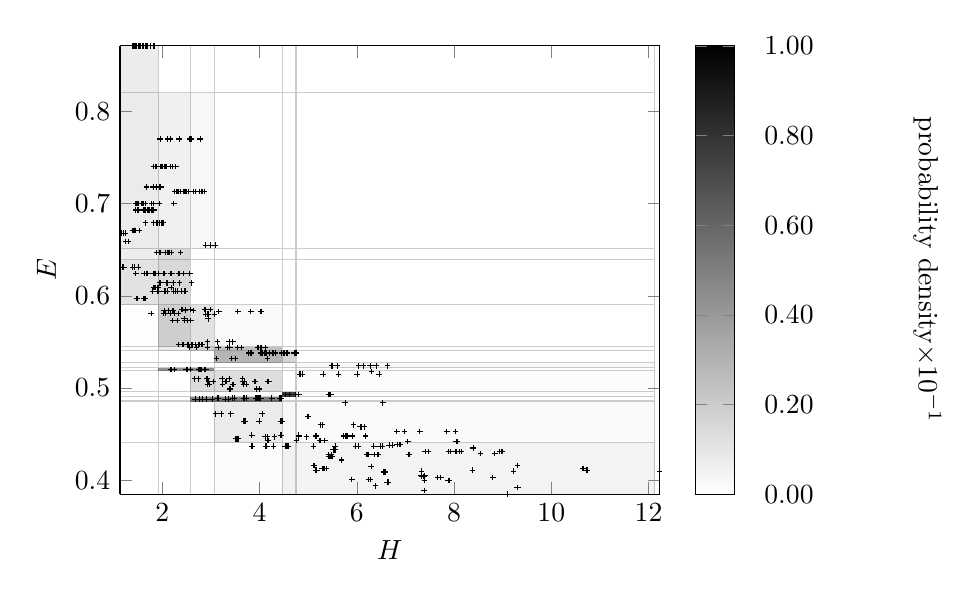
\begin{tikzpicture}
		\begin{axis}[
			view={0}{90},
			enlargelimits=0,
			zmin=0.0, zmax=1.0,
			xlabel=$H$,
			ylabel=$E$,
			colorbar,
			point meta min=0, point meta max=1.0,
			colormap={}{ gray(0cm)=(1); gray(1cm)=(0);},
			colorbar style={
			        ytick={0,0.2,...,1.01},
			        ylabel={probability density$ \times 10^{-1}$},
			        y label style={at={(axis description cs:6.5,0.5)},rotate=180,anchor=north},
			        yticklabel style={
			            text width=2.5em,
			            align=right,
			            /pgf/number format/.cd,
			                fixed,
			                fixed zerofill
			        }
			    }
			]

			\addplot3[patch,shader=faceted,patch type=rectangle] coordinates {(1.1296,0.3850,0.000000) (1.9204,0.3850,0.000000) (1.9204,0.4405,0.0000) (1.1296,0.4405,0.0000)};
			\addplot3[patch,shader=faceted,patch type=rectangle] coordinates {(1.1296,0.4405,0.000000) (1.9204,0.4405,0.000000) (1.9204,0.4860,0.0000) (1.1296,0.4860,0.0000)};
			\addplot3[patch,shader=faceted,patch type=rectangle] coordinates {(1.1296,0.4860,0.000000) (1.9204,0.4860,0.000000) (1.9204,0.4910,0.0000) (1.1296,0.4910,0.0000)};
			\addplot3[patch,shader=faceted,patch type=rectangle] coordinates {(1.1296,0.4910,0.000000) (1.9204,0.4910,0.000000) (1.9204,0.4960,0.0000) (1.1296,0.4960,0.0000)};
			\addplot3[patch,shader=faceted,patch type=rectangle] coordinates {(1.1296,0.4960,0.000000) (1.9204,0.4960,0.000000) (1.9204,0.5190,0.0000) (1.1296,0.5190,0.0000)};
			\addplot3[patch,shader=faceted,patch type=rectangle] coordinates {(1.1296,0.5190,0.000000) (1.9204,0.5190,0.000000) (1.9204,0.5220,0.0000) (1.1296,0.5220,0.0000)};
			\addplot3[patch,shader=faceted,patch type=rectangle] coordinates {(1.1296,0.5220,0.000000) (1.9204,0.5220,0.000000) (1.9204,0.5280,0.0000) (1.1296,0.5280,0.0000)};
			\addplot3[patch,shader=faceted,patch type=rectangle] coordinates {(1.1296,0.5280,0.000000) (1.9204,0.5280,0.000000) (1.9204,0.5410,0.0000) (1.1296,0.5410,0.0000)};
			\addplot3[patch,shader=faceted,patch type=rectangle] coordinates {(1.1296,0.5410,0.000000) (1.9204,0.5410,0.000000) (1.9204,0.5455,0.0000) (1.1296,0.5455,0.0000)};
			\addplot3[patch,shader=faceted,patch type=rectangle] coordinates {(1.1296,0.5455,0.006948) (1.9204,0.5455,0.006948) (1.9204,0.5910,0.0069) (1.1296,0.5910,0.0069)};
			\addplot3[patch,shader=faceted,patch type=rectangle] coordinates {(1.1296,0.5910,0.111972) (1.9204,0.5910,0.111972) (1.9204,0.6390,0.1120) (1.1296,0.6390,0.1120)};
			\addplot3[patch,shader=faceted,patch type=rectangle] coordinates {(1.1296,0.6390,0.068500) (1.9204,0.6390,0.068500) (1.9204,0.6510,0.0685) (1.1296,0.6510,0.0685)};
			\addplot3[patch,shader=faceted,patch type=rectangle] coordinates {(1.1296,0.6510,0.077593) (1.9204,0.6510,0.077593) (1.9204,0.8205,0.0776) (1.1296,0.8205,0.0776)};
			\addplot3[patch,shader=faceted,patch type=rectangle] coordinates {(1.1296,0.8205,0.075126) (1.9204,0.8205,0.075126) (1.9204,0.8710,0.0751) (1.1296,0.8710,0.0751)};

			\addplot3[patch,shader=faceted,patch type=rectangle] coordinates {(1.9204,0.3850,0.000000) (2.5884,0.3850,0.000000) (2.5884,0.4405,0.0000) (1.9204,0.4405,0.0000)};
			\addplot3[patch,shader=faceted,patch type=rectangle] coordinates {(1.9204,0.4405,0.000000) (2.5884,0.4405,0.000000) (2.5884,0.4860,0.0000) (1.9204,0.4860,0.0000)};
			\addplot3[patch,shader=faceted,patch type=rectangle] coordinates {(1.9204,0.4860,0.000000) (2.5884,0.4860,0.000000) (2.5884,0.4910,0.0000) (1.9204,0.4910,0.0000)};
			\addplot3[patch,shader=faceted,patch type=rectangle] coordinates {(1.9204,0.4910,0.000000) (2.5884,0.4910,0.000000) (2.5884,0.4960,0.0000) (1.9204,0.4960,0.0000)};
			\addplot3[patch,shader=faceted,patch type=rectangle] coordinates {(1.9204,0.4960,0.000000) (2.5884,0.4960,0.000000) (2.5884,0.5190,0.0000) (1.9204,0.5190,0.0000)};
			\addplot3[patch,shader=faceted,patch type=rectangle] coordinates {(1.9204,0.5190,0.424152) (2.5884,0.5190,0.424152) (2.5884,0.5220,0.4242) (1.9204,0.5220,0.4242)};
			\addplot3[patch,shader=faceted,patch type=rectangle] coordinates {(1.9204,0.5220,0.000000) (2.5884,0.5220,0.000000) (2.5884,0.5280,0.0000) (1.9204,0.5280,0.0000)};
			\addplot3[patch,shader=faceted,patch type=rectangle] coordinates {(1.9204,0.5280,0.000000) (2.5884,0.5280,0.000000) (2.5884,0.5410,0.0000) (1.9204,0.5410,0.0000)};
			\addplot3[patch,shader=faceted,patch type=rectangle] coordinates {(1.9204,0.5410,0.083167) (2.5884,0.5410,0.083167) (2.5884,0.5455,0.0832) (1.9204,0.5455,0.0832)};
			\addplot3[patch,shader=faceted,patch type=rectangle] coordinates {(1.9204,0.5455,0.190827) (2.5884,0.5455,0.190827) (2.5884,0.5910,0.1908) (1.9204,0.5910,0.1908)};
			\addplot3[patch,shader=faceted,patch type=rectangle] coordinates {(1.9204,0.5910,0.151260) (2.5884,0.5910,0.151260) (2.5884,0.6390,0.1513) (1.9204,0.6390,0.1513)};
			\addplot3[patch,shader=faceted,patch type=rectangle] coordinates {(1.9204,0.6390,0.149701) (2.5884,0.6390,0.149701) (2.5884,0.6510,0.1497) (1.9204,0.6510,0.1497)};
			\addplot3[patch,shader=faceted,patch type=rectangle] coordinates {(1.9204,0.6510,0.058732) (2.5884,0.6510,0.058732) (2.5884,0.8205,0.0587) (1.9204,0.8205,0.0587)};
			\addplot3[patch,shader=faceted,patch type=rectangle] coordinates {(1.9204,0.8205,0.000000) (2.5884,0.8205,0.000000) (2.5884,0.8710,0.0000) (1.9204,0.8710,0.0000)};

			\addplot3[patch,shader=faceted,patch type=rectangle] coordinates {(2.5884,0.3850,0.000000) (3.0793,0.3850,0.000000) (3.0793,0.4405,0.0000) (2.5884,0.4405,0.0000)};
			\addplot3[patch,shader=faceted,patch type=rectangle] coordinates {(2.5884,0.4405,0.000000) (3.0793,0.4405,0.000000) (3.0793,0.4860,0.0000) (2.5884,0.4860,0.0000)};
			\addplot3[patch,shader=faceted,patch type=rectangle] coordinates {(2.5884,0.4860,0.468479) (3.0793,0.4860,0.468479) (3.0793,0.4910,0.4685) (2.5884,0.4910,0.4685)};
			\addplot3[patch,shader=faceted,patch type=rectangle] coordinates {(2.5884,0.4910,0.000000) (3.0793,0.4910,0.000000) (3.0793,0.4960,0.0000) (2.5884,0.4960,0.0000)};
			\addplot3[patch,shader=faceted,patch type=rectangle] coordinates {(2.5884,0.4960,0.141695) (3.0793,0.4960,0.141695) (3.0793,0.5190,0.1417) (2.5884,0.5190,0.1417)};
			\addplot3[patch,shader=faceted,patch type=rectangle] coordinates {(2.5884,0.5190,0.441321) (3.0793,0.5190,0.441321) (3.0793,0.5220,0.4413) (2.5884,0.5220,0.4413)};
			\addplot3[patch,shader=faceted,patch type=rectangle] coordinates {(2.5884,0.5220,0.000000) (3.0793,0.5220,0.000000) (3.0793,0.5280,0.0000) (2.5884,0.5280,0.0000)};
			\addplot3[patch,shader=faceted,patch type=rectangle] coordinates {(2.5884,0.5280,0.000000) (3.0793,0.5280,0.000000) (3.0793,0.5410,0.0000) (2.5884,0.5410,0.0000)};
			\addplot3[patch,shader=faceted,patch type=rectangle] coordinates {(2.5884,0.5410,0.181055) (3.0793,0.5410,0.181055) (3.0793,0.5455,0.1811) (2.5884,0.5455,0.1811)};
			\addplot3[patch,shader=faceted,patch type=rectangle] coordinates {(2.5884,0.5455,0.111916) (3.0793,0.5455,0.111916) (3.0793,0.5910,0.1119) (2.5884,0.5910,0.1119)};
			\addplot3[patch,shader=faceted,patch type=rectangle] coordinates {(2.5884,0.5910,0.000000) (3.0793,0.5910,0.000000) (3.0793,0.6390,0.0000) (2.5884,0.6390,0.0000)};
			\addplot3[patch,shader=faceted,patch type=rectangle] coordinates {(2.5884,0.6390,0.000000) (3.0793,0.6390,0.000000) (3.0793,0.6510,0.0000) (2.5884,0.6510,0.0000)};
			\addplot3[patch,shader=faceted,patch type=rectangle] coordinates {(2.5884,0.6510,0.030042) (3.0793,0.6510,0.030042) (3.0793,0.8205,0.0300) (2.5884,0.8205,0.0300)};
			\addplot3[patch,shader=faceted,patch type=rectangle] coordinates {(2.5884,0.8205,0.000000) (3.0793,0.8205,0.000000) (3.0793,0.8710,0.0000) (2.5884,0.8710,0.0000)};

			\addplot3[patch,shader=faceted,patch type=rectangle] coordinates {(3.0793,0.3850,0.012861) (4.4802,0.3850,0.012861) (4.4802,0.4405,0.0129) (3.0793,0.4405,0.0129)};
			\addplot3[patch,shader=faceted,patch type=rectangle] coordinates {(3.0793,0.4405,0.077655) (4.4802,0.4405,0.077655) (4.4802,0.4860,0.0777) (3.0793,0.4860,0.0777)};
			\addplot3[patch,shader=faceted,patch type=rectangle] coordinates {(3.0793,0.4860,0.492523) (4.4802,0.4860,0.492523) (4.4802,0.4910,0.4925) (3.0793,0.4910,0.4925)};
			\addplot3[patch,shader=faceted,patch type=rectangle] coordinates {(3.0793,0.4910,0.000000) (4.4802,0.4910,0.000000) (4.4802,0.4960,0.0000) (3.0793,0.4960,0.0000)};
			\addplot3[patch,shader=faceted,patch type=rectangle] coordinates {(3.0793,0.4960,0.131898) (4.4802,0.4960,0.131898) (4.4802,0.5190,0.1319) (3.0793,0.5190,0.1319)};
			\addplot3[patch,shader=faceted,patch type=rectangle] coordinates {(3.0793,0.5190,0.000000) (4.4802,0.5190,0.000000) (4.4802,0.5220,0.0000) (3.0793,0.5220,0.0000)};
			\addplot3[patch,shader=faceted,patch type=rectangle] coordinates {(3.0793,0.5220,0.000000) (4.4802,0.5220,0.000000) (4.4802,0.5280,0.0000) (3.0793,0.5280,0.0000)};
			\addplot3[patch,shader=faceted,patch type=rectangle] coordinates {(3.0793,0.5280,0.288266) (4.4802,0.5280,0.288266) (4.4802,0.5410,0.2883) (3.0793,0.5410,0.2883)};
			\addplot3[patch,shader=faceted,patch type=rectangle] coordinates {(3.0793,0.5410,0.245865) (4.4802,0.5410,0.245865) (4.4802,0.5455,0.2459) (3.0793,0.5455,0.2459)};
			\addplot3[patch,shader=faceted,patch type=rectangle] coordinates {(3.0793,0.5455,0.021179) (4.4802,0.5455,0.021179) (4.4802,0.5910,0.0212) (3.0793,0.5910,0.0212)};
			\addplot3[patch,shader=faceted,patch type=rectangle] coordinates {(3.0793,0.5910,0.000000) (4.4802,0.5910,0.000000) (4.4802,0.6390,0.0000) (3.0793,0.6390,0.0000)};
			\addplot3[patch,shader=faceted,patch type=rectangle] coordinates {(3.0793,0.6390,0.000000) (4.4802,0.6390,0.000000) (4.4802,0.6510,0.0000) (3.0793,0.6510,0.0000)};
			\addplot3[patch,shader=faceted,patch type=rectangle] coordinates {(3.0793,0.6510,0.000000) (4.4802,0.6510,0.000000) (4.4802,0.8205,0.0000) (3.0793,0.8205,0.0000)};
			\addplot3[patch,shader=faceted,patch type=rectangle] coordinates {(3.0793,0.8205,0.000000) (4.4802,0.8205,0.000000) (4.4802,0.8710,0.0000) (3.0793,0.8710,0.0000)};

			\addplot3[patch,shader=faceted,patch type=rectangle] coordinates {(4.4802,0.3850,0.053387) (4.7503,0.3850,0.053387) (4.7503,0.4405,0.0534) (4.4802,0.4405,0.0534)};
			\addplot3[patch,shader=faceted,patch type=rectangle] coordinates {(4.4802,0.4405,0.028490) (4.7503,0.4405,0.028490) (4.7503,0.4860,0.0285) (4.4802,0.4860,0.0285)};
			\addplot3[patch,shader=faceted,patch type=rectangle] coordinates {(4.4802,0.4860,0.000000) (4.7503,0.4860,0.000000) (4.7503,0.4910,0.0000) (4.4802,0.4910,0.0000)};
			\addplot3[patch,shader=faceted,patch type=rectangle] coordinates {(4.4802,0.4910,0.740741) (4.7503,0.4910,0.740741) (4.7503,0.4960,0.7407) (4.4802,0.4960,0.7407)};
			\addplot3[patch,shader=faceted,patch type=rectangle] coordinates {(4.4802,0.4960,0.000000) (4.7503,0.4960,0.000000) (4.7503,0.5190,0.0000) (4.4802,0.5190,0.0000)};
			\addplot3[patch,shader=faceted,patch type=rectangle] coordinates {(4.4802,0.5190,0.000000) (4.7503,0.5190,0.000000) (4.7503,0.5220,0.0000) (4.4802,0.5220,0.0000)};
			\addplot3[patch,shader=faceted,patch type=rectangle] coordinates {(4.4802,0.5220,0.000000) (4.7503,0.5220,0.000000) (4.7503,0.5280,0.0000) (4.4802,0.5280,0.0000)};
			\addplot3[patch,shader=faceted,patch type=rectangle] coordinates {(4.4802,0.5280,0.170940) (4.7503,0.5280,0.170940) (4.7503,0.5410,0.1709) (4.4802,0.5410,0.1709)};
			\addplot3[patch,shader=faceted,patch type=rectangle] coordinates {(4.4802,0.5410,0.000000) (4.7503,0.5410,0.000000) (4.7503,0.5455,0.0000) (4.4802,0.5455,0.0000)};
			\addplot3[patch,shader=faceted,patch type=rectangle] coordinates {(4.4802,0.5455,0.000000) (4.7503,0.5455,0.000000) (4.7503,0.5910,0.0000) (4.4802,0.5910,0.0000)};
			\addplot3[patch,shader=faceted,patch type=rectangle] coordinates {(4.4802,0.5910,0.000000) (4.7503,0.5910,0.000000) (4.7503,0.6390,0.0000) (4.4802,0.6390,0.0000)};
			\addplot3[patch,shader=faceted,patch type=rectangle] coordinates {(4.4802,0.6390,0.000000) (4.7503,0.6390,0.000000) (4.7503,0.6510,0.0000) (4.4802,0.6510,0.0000)};
			\addplot3[patch,shader=faceted,patch type=rectangle] coordinates {(4.4802,0.6510,0.000000) (4.7503,0.6510,0.000000) (4.7503,0.8205,0.0000) (4.4802,0.8205,0.0000)};
			\addplot3[patch,shader=faceted,patch type=rectangle] coordinates {(4.4802,0.8205,0.000000) (4.7503,0.8205,0.000000) (4.7503,0.8710,0.0000) (4.4802,0.8710,0.0000)};

			\addplot3[patch,shader=faceted,patch type=rectangle] coordinates {(4.7503,0.3850,0.045434) (12.1265,0.3850,0.045434) (12.1265,0.4405,0.0454) (4.7503,0.4405,0.0454)};
			\addplot3[patch,shader=faceted,patch type=rectangle] coordinates {(4.7503,0.4405,0.018324) (12.1265,0.4405,0.018324) (12.1265,0.4860,0.0183) (4.7503,0.4860,0.0183)};
			\addplot3[patch,shader=faceted,patch type=rectangle] coordinates {(4.7503,0.4860,0.000000) (12.1265,0.4860,0.000000) (12.1265,0.4910,0.0000) (4.7503,0.4910,0.0000)};
			\addplot3[patch,shader=faceted,patch type=rectangle] coordinates {(4.7503,0.4910,0.012201) (12.1265,0.4910,0.012201) (12.1265,0.4960,0.0122) (4.7503,0.4960,0.0122)};
			\addplot3[patch,shader=faceted,patch type=rectangle] coordinates {(4.7503,0.4960,0.012378) (12.1265,0.4960,0.012378) (12.1265,0.5190,0.0124) (4.7503,0.5190,0.0124)};
			\addplot3[patch,shader=faceted,patch type=rectangle] coordinates {(4.7503,0.5190,0.000000) (12.1265,0.5190,0.000000) (12.1265,0.5220,0.0000) (4.7503,0.5220,0.0000)};
			\addplot3[patch,shader=faceted,patch type=rectangle] coordinates {(4.7503,0.5220,0.027114) (12.1265,0.5220,0.027114) (12.1265,0.5280,0.0271) (4.7503,0.5280,0.0271)};
			\addplot3[patch,shader=faceted,patch type=rectangle] coordinates {(4.7503,0.5280,0.000000) (12.1265,0.5280,0.000000) (12.1265,0.5410,0.0000) (4.7503,0.5410,0.0000)};
			\addplot3[patch,shader=faceted,patch type=rectangle] coordinates {(4.7503,0.5410,0.000000) (12.1265,0.5410,0.000000) (12.1265,0.5455,0.0000) (4.7503,0.5455,0.0000)};
			\addplot3[patch,shader=faceted,patch type=rectangle] coordinates {(4.7503,0.5455,0.000000) (12.1265,0.5455,0.000000) (12.1265,0.5910,0.0000) (4.7503,0.5910,0.0000)};
			\addplot3[patch,shader=faceted,patch type=rectangle] coordinates {(4.7503,0.5910,0.000000) (12.1265,0.5910,0.000000) (12.1265,0.6390,0.0000) (4.7503,0.6390,0.0000)};
			\addplot3[patch,shader=faceted,patch type=rectangle] coordinates {(4.7503,0.6390,0.000000) (12.1265,0.6390,0.000000) (12.1265,0.6510,0.0000) (4.7503,0.6510,0.0000)};
			\addplot3[patch,shader=faceted,patch type=rectangle] coordinates {(4.7503,0.6510,0.000000) (12.1265,0.6510,0.000000) (12.1265,0.8205,0.0000) (4.7503,0.8205,0.0000)};
			\addplot3[patch,shader=faceted,patch type=rectangle] coordinates {(4.7503,0.8205,0.000000) (12.1265,0.8205,0.000000) (12.1265,0.8710,0.0000) (4.7503,0.8710,0.0000)};

			\addplot3[mark=+, draw=none, mark size=1.0, jitter = 0.1] coordinates {
(4.090,0.538,1) (4.967,0.469,1) (4.967,0.469,1) (6.062,0.458,1) (6.062,0.458,1) (6.062,0.458,1) (5.561,0.524,1) (5.950,0.524,1) (6.082,0.524,1) (6.592,0.524,1) (6.347,0.524,1) (6.227,0.524,1) (5.451,0.524,1) (4.707,0.538,1) (4.462,0.538,1) (4.499,0.538,1) (4.499,0.538,1) (4.258,0.538,1) (3.796,0.538,1) (3.796,0.538,1) (3.798,0.538,1) (4.012,0.538,1) (3.977,0.538,1) (4.095,0.538,1) (4.400,0.538,1) (4.455,0.538,1) (4.682,0.538,1) (4.453,0.538,1) (4.455,0.538,1) (4.239,0.538,1) (4.233,0.538,1) (4.175,0.538,1) (3.990,0.538,1) (3.787,0.538,1) (3.760,0.538,1) (3.360,0.499,1) (3.378,0.499,1) (3.934,0.499,1) (3.847,0.499,1) (5.401,0.428,1) (5.401,0.428,1) (5.721,0.448,1) (5.721,0.448,1) (5.721,0.448,1) (5.721,0.448,1) (5.100,0.448,1) (5.100,0.448,1) (5.689,0.448,1) (5.870,0.448,1) (6.088,0.448,1) (6.815,0.439,1) (6.815,0.439,1) (6.815,0.439,1) (6.815,0.439,1) (7.320,0.410,1) (8.697,0.403,1) (9.188,0.410,1) (8.325,0.411,1) (7.815,0.453,1) (6.932,0.453,1) (7.225,0.453,1) (6.819,0.453,1) (7.226,0.453,1) (7.981,0.453,1) (9.223,0.416,1) (6.612,0.398,1) (6.612,0.398,1) (6.498,0.409,1) (6.498,0.409,1) (6.498,0.409,1) (5.287,0.413,1) (5.287,0.413,1) (5.287,0.413,1) (5.287,0.413,1) (4.252,0.437,1) (4.503,0.437,1) (4.052,0.437,1) (4.090,0.437,1) (5.014,0.437,1) (4.503,0.437,1) (5.401,0.426,1) (5.401,0.426,1) (5.401,0.426,1) (5.401,0.426,1) (4.779,0.449,1) (4.438,0.449,1) (4.427,0.449,1) (3.748,0.449,1) (3.422,0.489,1) (3.414,0.489,1) (3.092,0.489,1) (3.092,0.489,1) (3.666,0.464,1) (3.666,0.464,1) (3.615,0.464,1) (3.495,0.445,1) (3.495,0.445,1) (3.495,0.445,1) (3.495,0.445,1) (3.495,0.445,1) (2.778,0.520,1) (2.856,0.520,1) (2.715,0.520,1) (2.715,0.520,1) (2.421,0.520,1) (2.107,0.520,1) (2.211,0.520,1) (2.122,0.520,1) (2.433,0.520,1) (2.545,0.520,1) (2.778,0.520,1) (2.678,0.547,1) (2.353,0.547,1) (2.548,0.547,1) (2.256,0.547,1) (2.463,0.547,1) (2.730,0.547,1) (2.747,0.547,1) (2.478,0.547,1) (2.759,0.547,1) (2.258,0.581,1) (2.197,0.581,1) (2.087,0.581,1) (1.944,0.581,1) (2.006,0.581,1) (1.993,0.581,1) (1.757,0.581,1) (1.788,0.624,1) (1.813,0.624,1) (1.980,0.624,1) (2.119,0.624,1) (2.271,0.624,1) (2.327,0.624,1) (2.470,0.624,1) (2.346,0.624,1) (2.111,0.624,1) (1.967,0.624,1) (1.850,0.624,1) (1.669,0.624,1) (1.669,0.624,1) (1.612,0.624,1) (1.439,0.624,1) (1.322,0.871,1) (1.412,0.871,1) (1.346,0.871,1) (1.419,0.871,1) (1.517,0.871,1) (1.461,0.871,1) (1.530,0.871,1) (1.526,0.871,1) (1.618,0.871,1) (1.592,0.871,1) (1.610,0.871,1) (1.623,0.871,1) (1.749,0.871,1) (1.746,0.871,1) (1.736,0.871,1) (1.877,0.605,1) (1.757,0.605,1) (1.766,0.871,1) (1.798,0.605,1) (1.971,0.605,1) (2.041,0.605,1) (2.162,0.605,1) (2.422,0.605,1) (2.283,0.605,1) (2.046,0.605,1) (2.426,0.605,1) (2.100,0.605,1) (2.263,0.605,1) (2.426,0.605,1) (2.389,0.605,1) (2.596,0.510,1) (2.646,0.510,1) (2.702,0.510,1) (3.132,0.510,1) (3.555,0.510,1) (3.317,0.510,1) (2.915,0.510,1) (2.829,0.488,1) (2.741,0.488,1) (2.598,0.488,1) (2.701,0.488,1) (2.847,0.488,1) (2.988,0.488,1) (3.280,0.488,1) (3.199,0.488,1) (3.789,0.437,1) (4.567,0.437,1) (4.567,0.437,1) (6.480,0.437,1) (6.480,0.437,1) (6.480,0.437,1) (6.220,0.401,1) (6.220,0.401,1) (5.648,0.422,1) (7.309,0.404,1) (7.309,0.404,1) (7.309,0.404,1) (7.653,0.403,1) (7.653,0.403,1) (6.270,0.415,1) (6.270,0.415,1) (5.118,0.416,1) (5.118,0.416,1) (3.945,0.489,1) (4.355,0.489,1) (4.355,0.489,1) (4.239,0.489,1) (3.875,0.489,1) (3.877,0.489,1) (3.665,0.489,1) (3.653,0.489,1) (3.945,0.489,1) (3.587,0.489,1) (3.945,0.489,1) (3.112,0.550,1) (3.421,0.550,1) (2.889,0.550,1) (3.363,0.550,1) (2.862,0.507,1) (3.048,0.507,1) (3.272,0.507,1) (3.272,0.507,1) (2.894,0.504,1) (2.894,0.504,1) (3.216,0.504,1) (3.216,0.504,1) (3.375,0.504,1) (3.375,0.504,1) (3.671,0.504,1) (3.671,0.504,1) (3.838,0.507,1) (3.652,0.507,1) (3.652,0.507,1) (3.652,0.507,1) (4.148,0.507,1) (4.148,0.507,1) (6.190,0.428,1) (6.190,0.428,1) (6.336,0.428,1) (6.336,0.428,1) (7.035,0.428,1) (7.035,0.428,1) (7.955,0.431,1) (7.955,0.431,1) (8.056,0.431,1) (8.056,0.431,1) (7.827,0.431,1) (7.827,0.431,1) (7.397,0.431,1) (7.397,0.431,1) (8.907,0.431,1) (8.907,0.431,1) (9.220,0.392,1) (9.220,0.392,1) (6.336,0.394,1) (1.801,0.647,1) (1.895,0.647,1) (2.011,0.647,1) (2.112,0.647,1) (2.140,0.647,1) (2.288,0.647,1) (2.079,0.647,1) (1.930,0.647,1) (1.986,0.647,1) (2.133,0.647,1) (2.422,0.575,1) (2.872,0.575,1) (3.917,0.464,1) (4.429,0.464,1) (4.429,0.464,1) (3.917,0.464,1) (4.367,0.464,1) (4.078,0.447,1) (4.267,0.447,1) (4.787,0.447,1) (4.863,0.447,1) (4.140,0.447,1) (4.101,0.443,1) (4.695,0.443,1) (5.245,0.443,1) (5.212,0.443,1) (5.885,0.401,1) (7.307,0.400,1) (7.307,0.389,1) (9.089,0.385,1) (7.317,0.405,1) (7.317,0.405,1) (7.317,0.405,1) (5.117,0.411,1) (5.117,0.411,1) (5.117,0.411,1) (5.503,0.437,1) (5.503,0.437,1) (5.960,0.437,1) (5.960,0.437,1) (6.320,0.437,1) (7.828,0.400,1) (7.828,0.400,1) (7.828,0.400,1) (5.492,0.433,1) (5.492,0.433,1) (5.492,0.433,1) (4.022,0.472,1) (3.370,0.472,1) (3.099,0.472,1) (3.183,0.472,1) (3.317,0.544,1) (3.103,0.544,1) (2.519,0.544,1) (2.640,0.544,1) (2.834,0.544,1) (3.263,0.544,1) (3.602,0.544,1) (3.945,0.544,1) (3.999,0.544,1) (4.032,0.544,1) (3.533,0.544,1) (4.002,0.544,1) (4.540,0.493,1) (4.540,0.493,1) (4.721,0.493,1) (4.721,0.493,1) (4.721,0.493,1) (5.416,0.493,1) (5.416,0.493,1) (5.416,0.493,1) (5.215,0.460,1) (5.215,0.460,1) (5.874,0.460,1) (6.641,0.438,1) (6.641,0.438,1) (6.458,0.515,1) (6.458,0.515,1) (5.985,0.515,1) (5.231,0.515,1) (5.615,0.515,1) (4.812,0.515,1) (4.812,0.515,1) (4.812,0.515,1) (7.038,0.442,1) (6.267,0.518,1) (5.732,0.484,1) (6.465,0.484,1) (8.014,0.442,1) (8.014,0.442,1) (8.535,0.429,1) (8.344,0.435,1) (8.792,0.429,1) (8.792,0.429,1) (10.710,0.411,1) (10.710,0.411,1) (12.127,0.410,1) (10.586,0.413,1) (10.586,0.413,1) (2.122,0.770,1) (2.505,0.770,1) (2.723,0.770,1) (2.509,0.770,1) (2.518,0.770,1) (2.296,0.770,1) (2.104,0.770,1) (1.905,0.770,1) (1.905,0.718,1) (1.613,0.718,1) (1.752,0.718,1) (1.511,0.631,1) (1.333,0.631,1) (1.357,0.631,1) (1.202,0.631,1) (1.169,0.631,1) (1.130,0.668,1) (1.174,0.668,1) (1.137,0.668,1) (1.316,0.671,1) (1.345,0.671,1) (1.358,0.671,1) (1.386,0.671,1) (1.386,0.671,1) (1.417,0.671,1) (1.519,0.671,1) (1.580,0.700,1) (1.533,0.700,1) (1.440,0.700,1) (1.426,0.700,1) (1.467,0.700,1) (1.518,0.700,1) (1.589,0.700,1) (1.728,0.700,1) (1.927,0.700,1) (2.168,0.700,1) (1.770,0.700,1) (1.791,0.693,1) (1.782,0.693,1) (1.726,0.693,1) (1.677,0.693,1) (1.633,0.693,1) (1.490,0.693,1) (1.500,0.693,1) (1.589,0.693,1) (1.574,0.693,1) (1.639,0.693,1) (1.703,0.693,1) (1.607,0.693,1) (1.425,0.693,1) (1.178,0.659,1) (1.285,0.659,1) (1.455,0.597,1) (1.466,0.597,1) (1.413,0.597,1) (1.528,0.597,1) (1.554,0.597,1) (1.589,0.597,1) (1.658,0.693,1) (1.835,0.679,1) (1.819,0.679,1) (1.647,0.679,1) (1.803,0.679,1) (1.794,0.718,1) (1.859,0.718,1) (1.875,0.718,1) (1.951,0.614,1) (2.022,0.614,1) (2.063,0.584,1) (1.910,0.679,1) (1.998,0.584,1) (1.863,0.679,1) (1.936,0.679,1) (1.968,0.679,1) (2.053,0.584,1) (2.088,0.584,1) (2.200,0.584,1) (2.316,0.713,1) (2.222,0.713,1) (2.125,0.740,1) (2.003,0.740,1) (1.914,0.740,1) (1.821,0.740,1) (1.817,0.740,1) (1.866,0.740,1) (2.065,0.740,1) (2.005,0.740,1) (1.978,0.740,1) (1.896,0.740,1) (1.988,0.740,1) (2.072,0.740,1) (2.198,0.740,1) (2.262,0.713,1) (2.185,0.713,1) (2.324,0.713,1) (2.355,0.713,1) (2.368,0.713,1) (2.453,0.713,1) (2.496,0.713,1) (2.436,0.713,1) (2.581,0.713,1) (2.779,0.713,1) (2.783,0.713,1) (2.717,0.713,1) (2.598,0.713,1) (2.567,0.713,1) (2.734,0.713,1) (2.802,0.713,1) (2.963,0.655,1) (3.067,0.655,1) (2.872,0.655,1) (2.540,0.584,1) (2.908,0.580,1) (2.824,0.580,1) (3.033,0.580,1) (3.099,0.532,1) (2.897,0.580,1) (2.533,0.614,1) (2.430,0.584,1) (2.206,0.584,1) (2.305,0.614,1) (2.101,0.614,1) (2.171,0.614,1) (1.951,0.614,1) (3.424,0.532,1) (3.332,0.532,1) (3.411,0.532,1) (4.098,0.532,1) (3.724,0.583,1) (3.992,0.583,1) (3.546,0.583,1) (3.152,0.583,1) (1.821,0.609,1) (1.755,0.609,1) (1.823,0.609,1) (1.868,0.609,1) (2.110,0.609,1) (2.382,0.585,1) (2.382,0.585,1) (2.799,0.585,1) (2.799,0.585,1) (2.893,0.585,1) (2.409,0.585,1) (2.400,0.585,1) (2.498,0.585,1) (2.479,0.573,1) (2.288,0.573,1) (2.167,0.573,1) (2.389,0.573,1) (2.505,0.573,1) };
		\end{axis}
	\end{tikzpicture}

  \caption{
    The discretization policies for variables $H$ and $E$ learned using the optimal Bayesian approach on the fixed network shown in Figure~\ref{fig:housing_graph_1}.
    The variable $H$ possesses no overly repeated values, thus producing a cleaner discretization policy.
  }
  \label{fig:housing_exp1_distr_8_5}
\end{figure}

\subsubsection{Discretization while Learning Structure}
\label{subsubsec:housing_exp2}

Figure~\ref{fig:housing_graph_2} shows a learned Bayesian network structure and the corresponding numbers of intervals after discretization for each continuous variable.
Variable $D$ is neighborless is both the learned and fixed networks.
The continuous variables $C$, $E$, $J$ and $K$, which are all connected through $C$, have many discretization intervals.
Typically, when discretizing a variable, the expected number of discretization intervals is close to the highest cardinality among variables in its Markov blanket.
This naturally leads to clusters of variables with high numbers of discretization intervals.

\begin{figure}[ht]
  \centering
  \scalebox{0.8}{% model_pca.tex
%
% Copyright (C) 2012 Jaakko Luttinen
%
% This file may be distributed and/or modified
%
% 1. under the LaTeX Project Public License and/or
% 2. under the GNU General Public License.
%
% See the files LICENSE_LPPL and LICENSE_GPL for more details.

% PCA model

%\beginpgfgraphicnamed{model-pca}
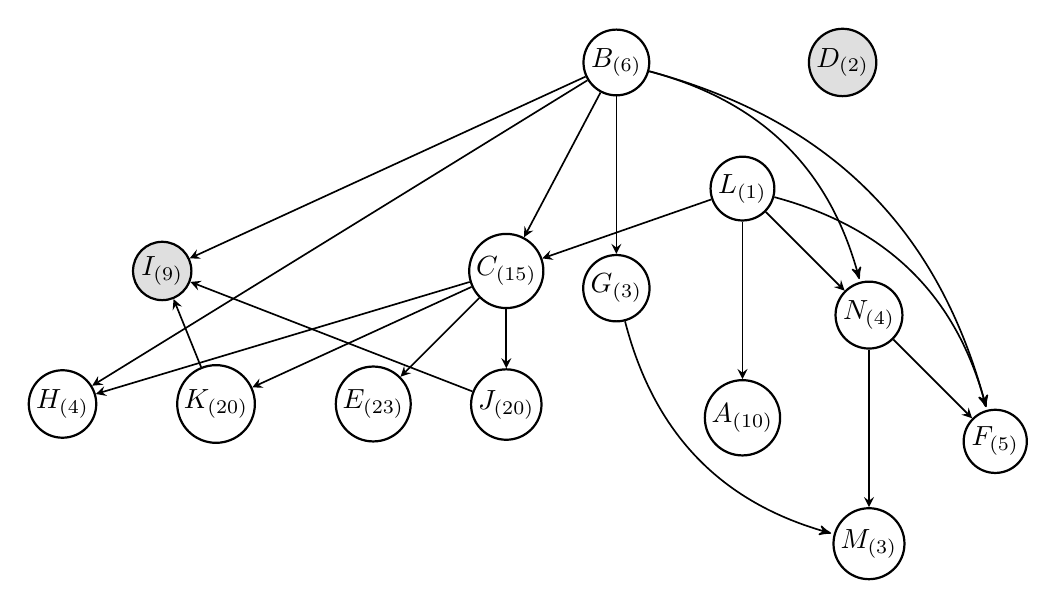
\begin{tikzpicture}[
      nodes={
        draw=black!20, thick, fill=white, font=\normalsize,
        minimum width=2.5em, minimum height=2em
      },
      rounded corners, semithick, >=stealth
      ]

	  \node[latent]          (c2) {$B_{(6)}$};
	  \node[obs, right = 2.0 of c2]  (c4){$D_{(2)}$};
	  \node[latent, below right = 1.0 and 1.0 of c2]  (c12){$L_{(1)}$};
	  \node[latent, below right = 1.0 and 1.0 of c12]  (c14){$N_{(4)}$};
	  \node[latent, below right = 1.0 and 1.0 of c14]  (c6){$F_{(5)}$};
	  \node[latent, below= 2.0 of c2]  (c7){$G_{(3)}$};
	  \node[latent, below = 2.0 of c12]  (c1){$A_{(10)}$};
	  \node[latent, below = 2.0 of c14]  (c13){$M_{(3)}$};
	  \node[latent, below left = 2.0 and 0.75 of c2] (c3){$C_{(15)}$};
	  \node[latent, below = 0.75 of c3]  (c10){$J_{(20)}$};
	  \node[latent, below left = 1.0 and 1.0 of c3] (c5){$E_{(23)}$};
	  \node[latent, left = 1.0 of c5] (c11){$K_{(20)}$};
	  \node[latent, left = 1.0 of c11] (c8){$H_{(4)}$};
	  \node[obs, left = 3.5 of c3] (c9){$I_{(9)}$};

  % Connect the nodes

  \edge {c2}{c9,c8,c3,c7};
  \draw[->,>=stealth', shorten >= 1pt] (c2) to[bend left](c14);
  \draw[->,>=stealth', shorten >= 1pt] (c2) to[bend left](c6);
  \edge {c12}{c3,c1,c14}
  \draw[->,>=stealth', shorten >= 1pt] (c12) to[bend left](c6);
  \edge {c14}{c13,c6}
  \draw[->,>=stealth', shorten >= 1pt] (c7) to[bend right](c13);
  \edge {c3} {c8,c11,c5,c10}
  \edge {c11,c10}{c9}
  %\edge {c2}{c9,c3,c7}
  %\draw[->,>=stealth', shorten >= 1pt] (c2) to[bend right](c10);
  %\draw[->,>=stealth', shorten >= 1pt] (c4) to[bend left](c5);  
  %\edge {c3}{c9,c10,c11};
  %\edge{c9}{c10,c11};
  %\draw[->,>=stealth', shorten >= 1pt] (c9) to[bend left](c5);
  %\draw[->,>=stealth', shorten >= 1pt] (c9) to[bend right](c2);
  %\edge {c10}{c11,c12};
  %\edge {c7}{c13};
  %\edge {c13}{c14};
  %\edge {c14,c1}{c6};
  %\edge {c1}{c6,c11,c8,c5};
  %\edge {c2}{c1};
  %\draw[->,>=stealth', shorten >= 1pt] (c12) to[bend right](c1);
  %\draw[->,>=stealth', shorten >= 1pt] (c1) to[bend right](c7);
  %\edge {p1,p2} {y} ; %
  %\edge {y} {c2} ;
  %\edge {y}{c1};



\end{tikzpicture}
%\endpgfgraphicnamed

%%% Local Variables: 
%%% mode: tex-pdf
%%% TeX-master: "example"
%%% End: 
}
  \caption{
    The discrete-valued Bayesian network learned from the Housing dataset using the optimal Bayesian method.
  }
  \label{fig:housing_graph_2}
\end{figure}

Figure~\ref{fig:housing_exp2_distr_3_5} and Figure~\ref{fig:housing_exp2_distr_8_5} show the discretization result on variables of the network in Figure~\ref{fig:housing_graph_2}.
Again, variable $C$ and $E$ have many discretization edges due to the repeated values.
Although the number of intervals after discretization on $H$ is less the number in Figure~\ref{fig:housing_exp1_distr_8_5}, it still captures the distribution of the raw data along with the discretization edges on $E$.

\begin{figure}[ht]
  \centering
  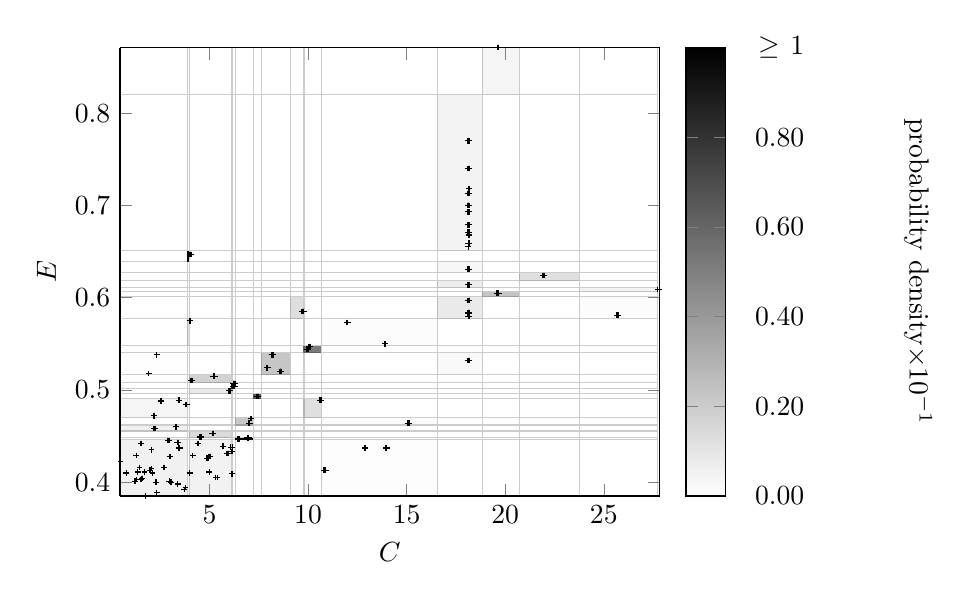
\begin{tikzpicture}
		\begin{axis}[
			view={0}{90},
			enlargelimits=0,
			zmin=0.0, zmax=1.0,
			xlabel=$C$,
			ylabel=$E$,
			colorbar,
			point meta min=0, point meta max=1,
			colormap={}{ gray(0cm)=(1); gray(1cm)=(0);},
			colorbar style={
			        ytick={0,0.2,...,1.01},
			        ylabel={probability density$ \times 10^{-1}$},
			        y label style={at={(axis description cs:6.5,0.5)},rotate=180,anchor=north},
			        yticklabels={\num{0.00},\num{0.20},\num{0.40},\num{0.60},\num{0.80},$\geq 1$},
			        yticklabel style={
			            text width=2.5em,
			            align=right,
			            /pgf/number format/.cd,
			                fixed,
			                fixed zerofill
			        }
			    }
			]

			\addplot3[patch,shader=faceted,patch type=rectangle] coordinates {(0.4600,0.3850,0.053045) (3.8750,0.3850,0.053045) (3.8750,0.4460,0.0530) (0.4600,0.4460,0.0530)};
			\addplot3[patch,shader=faceted,patch type=rectangle] coordinates {(0.4600,0.4460,0.000000) (3.8750,0.4460,0.000000) (3.8750,0.4485,0.0000) (0.4600,0.4485,0.0000)};
			\addplot3[patch,shader=faceted,patch type=rectangle] coordinates {(0.4600,0.4485,0.000000) (3.8750,0.4485,0.000000) (3.8750,0.4555,0.0000) (0.4600,0.4555,0.0000)};
			\addplot3[patch,shader=faceted,patch type=rectangle] coordinates {(0.4600,0.4555,0.058565) (3.8750,0.4555,0.058565) (3.8750,0.4620,0.0586) (0.4600,0.4620,0.0586)};
			\addplot3[patch,shader=faceted,patch type=rectangle] coordinates {(0.4600,0.4620,0.000000) (3.8750,0.4620,0.000000) (3.8750,0.4705,0.0000) (0.4600,0.4705,0.0000)};
			\addplot3[patch,shader=faceted,patch type=rectangle] coordinates {(0.4600,0.4705,0.040710) (3.8750,0.4705,0.040710) (3.8750,0.4910,0.0407) (0.4600,0.4910,0.0407)};
			\addplot3[patch,shader=faceted,patch type=rectangle] coordinates {(0.4600,0.4910,0.000000) (3.8750,0.4910,0.000000) (3.8750,0.4960,0.0000) (0.4600,0.4960,0.0000)};
			\addplot3[patch,shader=faceted,patch type=rectangle] coordinates {(0.4600,0.4960,0.000000) (3.8750,0.4960,0.000000) (3.8750,0.5015,0.0000) (0.4600,0.5015,0.0000)};
			\addplot3[patch,shader=faceted,patch type=rectangle] coordinates {(0.4600,0.5015,0.000000) (3.8750,0.5015,0.000000) (3.8750,0.5085,0.0000) (0.4600,0.5085,0.0000)};
			\addplot3[patch,shader=faceted,patch type=rectangle] coordinates {(0.4600,0.5085,0.000000) (3.8750,0.5085,0.000000) (3.8750,0.5165,0.0000) (0.4600,0.5165,0.0000)};
			\addplot3[patch,shader=faceted,patch type=rectangle] coordinates {(0.4600,0.5165,0.002988) (3.8750,0.5165,0.002988) (3.8750,0.5410,0.0030) (0.4600,0.5410,0.0030)};
			\addplot3[patch,shader=faceted,patch type=rectangle] coordinates {(0.4600,0.5410,0.000000) (3.8750,0.5410,0.000000) (3.8750,0.5485,0.0000) (0.4600,0.5485,0.0000)};
			\addplot3[patch,shader=faceted,patch type=rectangle] coordinates {(0.4600,0.5485,0.000000) (3.8750,0.5485,0.000000) (3.8750,0.5775,0.0000) (0.4600,0.5775,0.0000)};
			\addplot3[patch,shader=faceted,patch type=rectangle] coordinates {(0.4600,0.5775,0.000000) (3.8750,0.5775,0.000000) (3.8750,0.6010,0.0000) (0.4600,0.6010,0.0000)};
			\addplot3[patch,shader=faceted,patch type=rectangle] coordinates {(0.4600,0.6010,0.000000) (3.8750,0.6010,0.000000) (3.8750,0.6070,0.0000) (0.4600,0.6070,0.0000)};
			\addplot3[patch,shader=faceted,patch type=rectangle] coordinates {(0.4600,0.6070,0.000000) (3.8750,0.6070,0.000000) (3.8750,0.6115,0.0000) (0.4600,0.6115,0.0000)};
			\addplot3[patch,shader=faceted,patch type=rectangle] coordinates {(0.4600,0.6115,0.000000) (3.8750,0.6115,0.000000) (3.8750,0.6190,0.0000) (0.4600,0.6190,0.0000)};
			\addplot3[patch,shader=faceted,patch type=rectangle] coordinates {(0.4600,0.6190,0.000000) (3.8750,0.6190,0.000000) (3.8750,0.6275,0.0000) (0.4600,0.6275,0.0000)};
			\addplot3[patch,shader=faceted,patch type=rectangle] coordinates {(0.4600,0.6275,0.000000) (3.8750,0.6275,0.000000) (3.8750,0.6390,0.0000) (0.4600,0.6390,0.0000)};
			\addplot3[patch,shader=faceted,patch type=rectangle] coordinates {(0.4600,0.6390,0.000000) (3.8750,0.6390,0.000000) (3.8750,0.6510,0.0000) (0.4600,0.6510,0.0000)};
			\addplot3[patch,shader=faceted,patch type=rectangle] coordinates {(0.4600,0.6510,0.000000) (3.8750,0.6510,0.000000) (3.8750,0.8205,0.0000) (0.4600,0.8205,0.0000)};
			\addplot3[patch,shader=faceted,patch type=rectangle] coordinates {(0.4600,0.8205,0.000000) (3.8750,0.8205,0.000000) (3.8750,0.8710,0.0000) (0.4600,0.8710,0.0000)};

			\addplot3[patch,shader=faceted,patch type=rectangle] coordinates {(3.8750,0.3850,0.000000) (3.9850,0.3850,0.000000) (3.9850,0.4460,0.0000) (3.8750,0.4460,0.0000)};
			\addplot3[patch,shader=faceted,patch type=rectangle] coordinates {(3.8750,0.4460,0.000000) (3.9850,0.4460,0.000000) (3.9850,0.4485,0.0000) (3.8750,0.4485,0.0000)};
			\addplot3[patch,shader=faceted,patch type=rectangle] coordinates {(3.8750,0.4485,0.000000) (3.9850,0.4485,0.000000) (3.9850,0.4555,0.0000) (3.8750,0.4555,0.0000)};
			\addplot3[patch,shader=faceted,patch type=rectangle] coordinates {(3.8750,0.4555,0.000000) (3.9850,0.4555,0.000000) (3.9850,0.4620,0.0000) (3.8750,0.4620,0.0000)};
			\addplot3[patch,shader=faceted,patch type=rectangle] coordinates {(3.8750,0.4620,0.000000) (3.9850,0.4620,0.000000) (3.9850,0.4705,0.0000) (3.8750,0.4705,0.0000)};
			\addplot3[patch,shader=faceted,patch type=rectangle] coordinates {(3.8750,0.4705,0.000000) (3.9850,0.4705,0.000000) (3.9850,0.4910,0.0000) (3.8750,0.4910,0.0000)};
			\addplot3[patch,shader=faceted,patch type=rectangle] coordinates {(3.8750,0.4910,0.000000) (3.9850,0.4910,0.000000) (3.9850,0.4960,0.0000) (3.8750,0.4960,0.0000)};
			\addplot3[patch,shader=faceted,patch type=rectangle] coordinates {(3.8750,0.4960,0.000000) (3.9850,0.4960,0.000000) (3.9850,0.5015,0.0000) (3.8750,0.5015,0.0000)};
			\addplot3[patch,shader=faceted,patch type=rectangle] coordinates {(3.8750,0.5015,0.000000) (3.9850,0.5015,0.000000) (3.9850,0.5085,0.0000) (3.8750,0.5085,0.0000)};
			\addplot3[patch,shader=faceted,patch type=rectangle] coordinates {(3.8750,0.5085,0.000000) (3.9850,0.5085,0.000000) (3.9850,0.5165,0.0000) (3.8750,0.5165,0.0000)};
			\addplot3[patch,shader=faceted,patch type=rectangle] coordinates {(3.8750,0.5165,0.000000) (3.9850,0.5165,0.000000) (3.9850,0.5410,0.0000) (3.8750,0.5410,0.0000)};
			\addplot3[patch,shader=faceted,patch type=rectangle] coordinates {(3.8750,0.5410,0.000000) (3.9850,0.5410,0.000000) (3.9850,0.5485,0.0000) (3.8750,0.5485,0.0000)};
			\addplot3[patch,shader=faceted,patch type=rectangle] coordinates {(3.8750,0.5485,0.109718) (3.9850,0.5485,0.109718) (3.9850,0.5775,0.1097) (3.8750,0.5775,0.1097)};
			\addplot3[patch,shader=faceted,patch type=rectangle] coordinates {(3.8750,0.5775,0.000000) (3.9850,0.5775,0.000000) (3.9850,0.6010,0.0000) (3.8750,0.6010,0.0000)};
			\addplot3[patch,shader=faceted,patch type=rectangle] coordinates {(3.8750,0.6010,0.000000) (3.9850,0.6010,0.000000) (3.9850,0.6070,0.0000) (3.8750,0.6070,0.0000)};
			\addplot3[patch,shader=faceted,patch type=rectangle] coordinates {(3.8750,0.6070,0.000000) (3.9850,0.6070,0.000000) (3.9850,0.6115,0.0000) (3.8750,0.6115,0.0000)};
			\addplot3[patch,shader=faceted,patch type=rectangle] coordinates {(3.8750,0.6115,0.000000) (3.9850,0.6115,0.000000) (3.9850,0.6190,0.0000) (3.8750,0.6190,0.0000)};
			\addplot3[patch,shader=faceted,patch type=rectangle] coordinates {(3.8750,0.6190,0.000000) (3.9850,0.6190,0.000000) (3.9850,0.6275,0.0000) (3.8750,0.6275,0.0000)};
			\addplot3[patch,shader=faceted,patch type=rectangle] coordinates {(3.8750,0.6275,0.000000) (3.9850,0.6275,0.000000) (3.9850,0.6390,0.0000) (3.8750,0.6390,0.0000)};
			% \addplot3[patch,shader=faceted,patch type=rectangle] coordinates {(3.8750,0.6390,1.704545) (3.9850,0.6390,1.704545) (3.9850,0.6510,1.7045) (3.8750,0.6510,1.7045)};
			\addplot3[patch,shader=faceted,patch type=rectangle] coordinates {(3.8750,0.6390,1.000000) (3.9850,0.6390,1.000000) (3.9850,0.6510,1.0000) (3.8750,0.6510,1.0000)};
			\addplot3[patch,shader=faceted,patch type=rectangle] coordinates {(3.8750,0.6510,0.000000) (3.9850,0.6510,0.000000) (3.9850,0.8205,0.0000) (3.8750,0.8205,0.0000)};
			\addplot3[patch,shader=faceted,patch type=rectangle] coordinates {(3.8750,0.8205,0.000000) (3.9850,0.8205,0.000000) (3.9850,0.8710,0.0000) (3.8750,0.8710,0.0000)};

			\addplot3[patch,shader=faceted,patch type=rectangle] coordinates {(3.9850,0.3850,0.051609) (6.1450,0.3850,0.051609) (6.1450,0.4460,0.0516) (3.9850,0.4460,0.0516)};
			\addplot3[patch,shader=faceted,patch type=rectangle] coordinates {(3.9850,0.4460,0.000000) (6.1450,0.4460,0.000000) (6.1450,0.4485,0.0000) (3.9850,0.4485,0.0000)};
			\addplot3[patch,shader=faceted,patch type=rectangle] coordinates {(3.9850,0.4485,0.138889) (6.1450,0.4485,0.138889) (6.1450,0.4555,0.1389) (3.9850,0.4555,0.1389)};
			\addplot3[patch,shader=faceted,patch type=rectangle] coordinates {(3.9850,0.4555,0.000000) (6.1450,0.4555,0.000000) (6.1450,0.4620,0.0000) (3.9850,0.4620,0.0000)};
			\addplot3[patch,shader=faceted,patch type=rectangle] coordinates {(3.9850,0.4620,0.000000) (6.1450,0.4620,0.000000) (6.1450,0.4705,0.0000) (3.9850,0.4705,0.0000)};
			\addplot3[patch,shader=faceted,patch type=rectangle] coordinates {(3.9850,0.4705,0.000000) (6.1450,0.4705,0.000000) (6.1450,0.4910,0.0000) (3.9850,0.4910,0.0000)};
			\addplot3[patch,shader=faceted,patch type=rectangle] coordinates {(3.9850,0.4910,0.000000) (6.1450,0.4910,0.000000) (6.1450,0.4960,0.0000) (3.9850,0.4960,0.0000)};
			\addplot3[patch,shader=faceted,patch type=rectangle] coordinates {(3.9850,0.4960,0.079966) (6.1450,0.4960,0.079966) (6.1450,0.5015,0.0800) (3.9850,0.5015,0.0800)};
			\addplot3[patch,shader=faceted,patch type=rectangle] coordinates {(3.9850,0.5015,0.000000) (6.1450,0.5015,0.000000) (6.1450,0.5085,0.0000) (3.9850,0.5085,0.0000)};
			\addplot3[patch,shader=faceted,patch type=rectangle] coordinates {(3.9850,0.5085,0.173611) (6.1450,0.5085,0.173611) (6.1450,0.5165,0.1736) (3.9850,0.5165,0.1736)};
			\addplot3[patch,shader=faceted,patch type=rectangle] coordinates {(3.9850,0.5165,0.000000) (6.1450,0.5165,0.000000) (6.1450,0.5410,0.0000) (3.9850,0.5410,0.0000)};
			\addplot3[patch,shader=faceted,patch type=rectangle] coordinates {(3.9850,0.5410,0.000000) (6.1450,0.5410,0.000000) (6.1450,0.5485,0.0000) (3.9850,0.5485,0.0000)};
			\addplot3[patch,shader=faceted,patch type=rectangle] coordinates {(3.9850,0.5485,0.000000) (6.1450,0.5485,0.000000) (6.1450,0.5775,0.0000) (3.9850,0.5775,0.0000)};
			\addplot3[patch,shader=faceted,patch type=rectangle] coordinates {(3.9850,0.5775,0.000000) (6.1450,0.5775,0.000000) (6.1450,0.6010,0.0000) (3.9850,0.6010,0.0000)};
			\addplot3[patch,shader=faceted,patch type=rectangle] coordinates {(3.9850,0.6010,0.000000) (6.1450,0.6010,0.000000) (6.1450,0.6070,0.0000) (3.9850,0.6070,0.0000)};
			\addplot3[patch,shader=faceted,patch type=rectangle] coordinates {(3.9850,0.6070,0.000000) (6.1450,0.6070,0.000000) (6.1450,0.6115,0.0000) (3.9850,0.6115,0.0000)};
			\addplot3[patch,shader=faceted,patch type=rectangle] coordinates {(3.9850,0.6115,0.000000) (6.1450,0.6115,0.000000) (6.1450,0.6190,0.0000) (3.9850,0.6190,0.0000)};
			\addplot3[patch,shader=faceted,patch type=rectangle] coordinates {(3.9850,0.6190,0.000000) (6.1450,0.6190,0.000000) (6.1450,0.6275,0.0000) (3.9850,0.6275,0.0000)};
			\addplot3[patch,shader=faceted,patch type=rectangle] coordinates {(3.9850,0.6275,0.000000) (6.1450,0.6275,0.000000) (6.1450,0.6390,0.0000) (3.9850,0.6390,0.0000)};
			\addplot3[patch,shader=faceted,patch type=rectangle] coordinates {(3.9850,0.6390,0.000000) (6.1450,0.6390,0.000000) (6.1450,0.6510,0.0000) (3.9850,0.6510,0.0000)};
			\addplot3[patch,shader=faceted,patch type=rectangle] coordinates {(3.9850,0.6510,0.000000) (6.1450,0.6510,0.000000) (6.1450,0.8205,0.0000) (3.9850,0.8205,0.0000)};
			\addplot3[patch,shader=faceted,patch type=rectangle] coordinates {(3.9850,0.8205,0.000000) (6.1450,0.8205,0.000000) (6.1450,0.8710,0.0000) (3.9850,0.8710,0.0000)};

			\addplot3[patch,shader=faceted,patch type=rectangle] coordinates {(6.1450,0.3850,0.000000) (6.3050,0.3850,0.000000) (6.3050,0.4460,0.0000) (6.1450,0.4460,0.0000)};
			\addplot3[patch,shader=faceted,patch type=rectangle] coordinates {(6.1450,0.4460,0.000000) (6.3050,0.4460,0.000000) (6.3050,0.4485,0.0000) (6.1450,0.4485,0.0000)};
			\addplot3[patch,shader=faceted,patch type=rectangle] coordinates {(6.1450,0.4485,0.000000) (6.3050,0.4485,0.000000) (6.3050,0.4555,0.0000) (6.1450,0.4555,0.0000)};
			\addplot3[patch,shader=faceted,patch type=rectangle] coordinates {(6.1450,0.4555,0.000000) (6.3050,0.4555,0.000000) (6.3050,0.4620,0.0000) (6.1450,0.4620,0.0000)};
			\addplot3[patch,shader=faceted,patch type=rectangle] coordinates {(6.1450,0.4620,0.000000) (6.3050,0.4620,0.000000) (6.3050,0.4705,0.0000) (6.1450,0.4705,0.0000)};
			\addplot3[patch,shader=faceted,patch type=rectangle] coordinates {(6.1450,0.4705,0.000000) (6.3050,0.4705,0.000000) (6.3050,0.4910,0.0000) (6.1450,0.4910,0.0000)};
			\addplot3[patch,shader=faceted,patch type=rectangle] coordinates {(6.1450,0.4910,0.000000) (6.3050,0.4910,0.000000) (6.3050,0.4960,0.0000) (6.1450,0.4960,0.0000)};
			\addplot3[patch,shader=faceted,patch type=rectangle] coordinates {(6.1450,0.4960,0.000000) (6.3050,0.4960,0.000000) (6.3050,0.5015,0.0000) (6.1450,0.5015,0.0000)};
			\addplot3[patch,shader=faceted,patch type=rectangle] coordinates {(6.1450,0.5015,3.660714) (6.3050,0.5015,3.660714) (6.3050,0.5085,3.6607) (6.1450,0.5085,3.6607)};
			\addplot3[patch,shader=faceted,patch type=rectangle] coordinates {(6.1450,0.5085,0.000000) (6.3050,0.5085,0.000000) (6.3050,0.5165,0.0000) (6.1450,0.5165,0.0000)};
			\addplot3[patch,shader=faceted,patch type=rectangle] coordinates {(6.1450,0.5165,0.000000) (6.3050,0.5165,0.000000) (6.3050,0.5410,0.0000) (6.1450,0.5410,0.0000)};
			\addplot3[patch,shader=faceted,patch type=rectangle] coordinates {(6.1450,0.5410,0.000000) (6.3050,0.5410,0.000000) (6.3050,0.5485,0.0000) (6.1450,0.5485,0.0000)};
			\addplot3[patch,shader=faceted,patch type=rectangle] coordinates {(6.1450,0.5485,0.000000) (6.3050,0.5485,0.000000) (6.3050,0.5775,0.0000) (6.1450,0.5775,0.0000)};
			\addplot3[patch,shader=faceted,patch type=rectangle] coordinates {(6.1450,0.5775,0.000000) (6.3050,0.5775,0.000000) (6.3050,0.6010,0.0000) (6.1450,0.6010,0.0000)};
			\addplot3[patch,shader=faceted,patch type=rectangle] coordinates {(6.1450,0.6010,0.000000) (6.3050,0.6010,0.000000) (6.3050,0.6070,0.0000) (6.1450,0.6070,0.0000)};
			\addplot3[patch,shader=faceted,patch type=rectangle] coordinates {(6.1450,0.6070,0.000000) (6.3050,0.6070,0.000000) (6.3050,0.6115,0.0000) (6.1450,0.6115,0.0000)};
			\addplot3[patch,shader=faceted,patch type=rectangle] coordinates {(6.1450,0.6115,0.000000) (6.3050,0.6115,0.000000) (6.3050,0.6190,0.0000) (6.1450,0.6190,0.0000)};
			\addplot3[patch,shader=faceted,patch type=rectangle] coordinates {(6.1450,0.6190,0.000000) (6.3050,0.6190,0.000000) (6.3050,0.6275,0.0000) (6.1450,0.6275,0.0000)};
			\addplot3[patch,shader=faceted,patch type=rectangle] coordinates {(6.1450,0.6275,0.000000) (6.3050,0.6275,0.000000) (6.3050,0.6390,0.0000) (6.1450,0.6390,0.0000)};
			\addplot3[patch,shader=faceted,patch type=rectangle] coordinates {(6.1450,0.6390,0.000000) (6.3050,0.6390,0.000000) (6.3050,0.6510,0.0000) (6.1450,0.6510,0.0000)};
			\addplot3[patch,shader=faceted,patch type=rectangle] coordinates {(6.1450,0.6510,0.000000) (6.3050,0.6510,0.000000) (6.3050,0.8205,0.0000) (6.1450,0.8205,0.0000)};
			\addplot3[patch,shader=faceted,patch type=rectangle] coordinates {(6.1450,0.8205,0.000000) (6.3050,0.8205,0.000000) (6.3050,0.8710,0.0000) (6.1450,0.8710,0.0000)};

			\addplot3[patch,shader=faceted,patch type=rectangle] coordinates {(6.3050,0.3850,0.000000) (7.2250,0.3850,0.000000) (7.2250,0.4460,0.0000) (6.3050,0.4460,0.0000)};
			% \addplot3[patch,shader=faceted,patch type=rectangle] coordinates {(6.3050,0.4460,1.239130) (7.2250,0.4460,1.239130) (7.2250,0.4485,1.2391) (6.3050,0.4485,1.2391)};
			\addplot3[patch,shader=faceted,patch type=rectangle] coordinates {(6.3050,0.4460,1.000000) (7.2250,0.4460,1.000000) (7.2250,0.4485,1.0000) (6.3050,0.4485,1.0000)};
			\addplot3[patch,shader=faceted,patch type=rectangle] coordinates {(6.3050,0.4485,0.000000) (7.2250,0.4485,0.000000) (7.2250,0.4555,0.0000) (6.3050,0.4555,0.0000)};
			\addplot3[patch,shader=faceted,patch type=rectangle] coordinates {(6.3050,0.4555,0.000000) (7.2250,0.4555,0.000000) (7.2250,0.4620,0.0000) (6.3050,0.4620,0.0000)};
			\addplot3[patch,shader=faceted,patch type=rectangle] coordinates {(6.3050,0.4620,0.210997) (7.2250,0.4620,0.210997) (7.2250,0.4705,0.2110) (6.3050,0.4705,0.2110)};
			\addplot3[patch,shader=faceted,patch type=rectangle] coordinates {(6.3050,0.4705,0.000000) (7.2250,0.4705,0.000000) (7.2250,0.4910,0.0000) (6.3050,0.4910,0.0000)};
			\addplot3[patch,shader=faceted,patch type=rectangle] coordinates {(6.3050,0.4910,0.000000) (7.2250,0.4910,0.000000) (7.2250,0.4960,0.0000) (6.3050,0.4960,0.0000)};
			\addplot3[patch,shader=faceted,patch type=rectangle] coordinates {(6.3050,0.4960,0.000000) (7.2250,0.4960,0.000000) (7.2250,0.5015,0.0000) (6.3050,0.5015,0.0000)};
			\addplot3[patch,shader=faceted,patch type=rectangle] coordinates {(6.3050,0.5015,0.000000) (7.2250,0.5015,0.000000) (7.2250,0.5085,0.0000) (6.3050,0.5085,0.0000)};
			\addplot3[patch,shader=faceted,patch type=rectangle] coordinates {(6.3050,0.5085,0.000000) (7.2250,0.5085,0.000000) (7.2250,0.5165,0.0000) (6.3050,0.5165,0.0000)};
			\addplot3[patch,shader=faceted,patch type=rectangle] coordinates {(6.3050,0.5165,0.000000) (7.2250,0.5165,0.000000) (7.2250,0.5410,0.0000) (6.3050,0.5410,0.0000)};
			\addplot3[patch,shader=faceted,patch type=rectangle] coordinates {(6.3050,0.5410,0.000000) (7.2250,0.5410,0.000000) (7.2250,0.5485,0.0000) (6.3050,0.5485,0.0000)};
			\addplot3[patch,shader=faceted,patch type=rectangle] coordinates {(6.3050,0.5485,0.000000) (7.2250,0.5485,0.000000) (7.2250,0.5775,0.0000) (6.3050,0.5775,0.0000)};
			\addplot3[patch,shader=faceted,patch type=rectangle] coordinates {(6.3050,0.5775,0.000000) (7.2250,0.5775,0.000000) (7.2250,0.6010,0.0000) (6.3050,0.6010,0.0000)};
			\addplot3[patch,shader=faceted,patch type=rectangle] coordinates {(6.3050,0.6010,0.000000) (7.2250,0.6010,0.000000) (7.2250,0.6070,0.0000) (6.3050,0.6070,0.0000)};
			\addplot3[patch,shader=faceted,patch type=rectangle] coordinates {(6.3050,0.6070,0.000000) (7.2250,0.6070,0.000000) (7.2250,0.6115,0.0000) (6.3050,0.6115,0.0000)};
			\addplot3[patch,shader=faceted,patch type=rectangle] coordinates {(6.3050,0.6115,0.000000) (7.2250,0.6115,0.000000) (7.2250,0.6190,0.0000) (6.3050,0.6190,0.0000)};
			\addplot3[patch,shader=faceted,patch type=rectangle] coordinates {(6.3050,0.6190,0.000000) (7.2250,0.6190,0.000000) (7.2250,0.6275,0.0000) (6.3050,0.6275,0.0000)};
			\addplot3[patch,shader=faceted,patch type=rectangle] coordinates {(6.3050,0.6275,0.000000) (7.2250,0.6275,0.000000) (7.2250,0.6390,0.0000) (6.3050,0.6390,0.0000)};
			\addplot3[patch,shader=faceted,patch type=rectangle] coordinates {(6.3050,0.6390,0.000000) (7.2250,0.6390,0.000000) (7.2250,0.6510,0.0000) (6.3050,0.6510,0.0000)};
			\addplot3[patch,shader=faceted,patch type=rectangle] coordinates {(6.3050,0.6510,0.000000) (7.2250,0.6510,0.000000) (7.2250,0.8205,0.0000) (6.3050,0.8205,0.0000)};
			\addplot3[patch,shader=faceted,patch type=rectangle] coordinates {(6.3050,0.8205,0.000000) (7.2250,0.8205,0.000000) (7.2250,0.8710,0.0000) (6.3050,0.8710,0.0000)};

			\addplot3[patch,shader=faceted,patch type=rectangle] coordinates {(7.2250,0.3850,0.000000) (7.6250,0.3850,0.000000) (7.6250,0.4460,0.0000) (7.2250,0.4460,0.0000)};
			\addplot3[patch,shader=faceted,patch type=rectangle] coordinates {(7.2250,0.4460,0.000000) (7.6250,0.4460,0.000000) (7.6250,0.4485,0.0000) (7.2250,0.4485,0.0000)};
			\addplot3[patch,shader=faceted,patch type=rectangle] coordinates {(7.2250,0.4485,0.000000) (7.6250,0.4485,0.000000) (7.6250,0.4555,0.0000) (7.2250,0.4555,0.0000)};
			\addplot3[patch,shader=faceted,patch type=rectangle] coordinates {(7.2250,0.4555,0.000000) (7.6250,0.4555,0.000000) (7.6250,0.4620,0.0000) (7.2250,0.4620,0.0000)};
			\addplot3[patch,shader=faceted,patch type=rectangle] coordinates {(7.2250,0.4620,0.000000) (7.6250,0.4620,0.000000) (7.6250,0.4705,0.0000) (7.2250,0.4705,0.0000)};
			\addplot3[patch,shader=faceted,patch type=rectangle] coordinates {(7.2250,0.4705,0.000000) (7.6250,0.4705,0.000000) (7.6250,0.4910,0.0000) (7.2250,0.4910,0.0000)};
			\addplot3[patch,shader=faceted,patch type=rectangle] coordinates {(7.2250,0.4910,0.625000) (7.6250,0.4910,0.625000) (7.6250,0.4960,0.6250) (7.2250,0.4960,0.6250)};
			\addplot3[patch,shader=faceted,patch type=rectangle] coordinates {(7.2250,0.4960,0.000000) (7.6250,0.4960,0.000000) (7.6250,0.5015,0.0000) (7.2250,0.5015,0.0000)};
			\addplot3[patch,shader=faceted,patch type=rectangle] coordinates {(7.2250,0.5015,0.000000) (7.6250,0.5015,0.000000) (7.6250,0.5085,0.0000) (7.2250,0.5085,0.0000)};
			\addplot3[patch,shader=faceted,patch type=rectangle] coordinates {(7.2250,0.5085,0.000000) (7.6250,0.5085,0.000000) (7.6250,0.5165,0.0000) (7.2250,0.5165,0.0000)};
			\addplot3[patch,shader=faceted,patch type=rectangle] coordinates {(7.2250,0.5165,0.000000) (7.6250,0.5165,0.000000) (7.6250,0.5410,0.0000) (7.2250,0.5410,0.0000)};
			\addplot3[patch,shader=faceted,patch type=rectangle] coordinates {(7.2250,0.5410,0.000000) (7.6250,0.5410,0.000000) (7.6250,0.5485,0.0000) (7.2250,0.5485,0.0000)};
			\addplot3[patch,shader=faceted,patch type=rectangle] coordinates {(7.2250,0.5485,0.000000) (7.6250,0.5485,0.000000) (7.6250,0.5775,0.0000) (7.2250,0.5775,0.0000)};
			\addplot3[patch,shader=faceted,patch type=rectangle] coordinates {(7.2250,0.5775,0.000000) (7.6250,0.5775,0.000000) (7.6250,0.6010,0.0000) (7.2250,0.6010,0.0000)};
			\addplot3[patch,shader=faceted,patch type=rectangle] coordinates {(7.2250,0.6010,0.000000) (7.6250,0.6010,0.000000) (7.6250,0.6070,0.0000) (7.2250,0.6070,0.0000)};
			\addplot3[patch,shader=faceted,patch type=rectangle] coordinates {(7.2250,0.6070,0.000000) (7.6250,0.6070,0.000000) (7.6250,0.6115,0.0000) (7.2250,0.6115,0.0000)};
			\addplot3[patch,shader=faceted,patch type=rectangle] coordinates {(7.2250,0.6115,0.000000) (7.6250,0.6115,0.000000) (7.6250,0.6190,0.0000) (7.2250,0.6190,0.0000)};
			\addplot3[patch,shader=faceted,patch type=rectangle] coordinates {(7.2250,0.6190,0.000000) (7.6250,0.6190,0.000000) (7.6250,0.6275,0.0000) (7.2250,0.6275,0.0000)};
			\addplot3[patch,shader=faceted,patch type=rectangle] coordinates {(7.2250,0.6275,0.000000) (7.6250,0.6275,0.000000) (7.6250,0.6390,0.0000) (7.2250,0.6390,0.0000)};
			\addplot3[patch,shader=faceted,patch type=rectangle] coordinates {(7.2250,0.6390,0.000000) (7.6250,0.6390,0.000000) (7.6250,0.6510,0.0000) (7.2250,0.6510,0.0000)};
			\addplot3[patch,shader=faceted,patch type=rectangle] coordinates {(7.2250,0.6510,0.000000) (7.6250,0.6510,0.000000) (7.6250,0.8205,0.0000) (7.2250,0.8205,0.0000)};
			\addplot3[patch,shader=faceted,patch type=rectangle] coordinates {(7.2250,0.8205,0.000000) (7.6250,0.8205,0.000000) (7.6250,0.8710,0.0000) (7.2250,0.8710,0.0000)};

			\addplot3[patch,shader=faceted,patch type=rectangle] coordinates {(7.6250,0.3850,0.000000) (9.1250,0.3850,0.000000) (9.1250,0.4460,0.0000) (7.6250,0.4460,0.0000)};
			\addplot3[patch,shader=faceted,patch type=rectangle] coordinates {(7.6250,0.4460,0.000000) (9.1250,0.4460,0.000000) (9.1250,0.4485,0.0000) (7.6250,0.4485,0.0000)};
			\addplot3[patch,shader=faceted,patch type=rectangle] coordinates {(7.6250,0.4485,0.000000) (9.1250,0.4485,0.000000) (9.1250,0.4555,0.0000) (7.6250,0.4555,0.0000)};
			\addplot3[patch,shader=faceted,patch type=rectangle] coordinates {(7.6250,0.4555,0.000000) (9.1250,0.4555,0.000000) (9.1250,0.4620,0.0000) (7.6250,0.4620,0.0000)};
			\addplot3[patch,shader=faceted,patch type=rectangle] coordinates {(7.6250,0.4620,0.000000) (9.1250,0.4620,0.000000) (9.1250,0.4705,0.0000) (7.6250,0.4705,0.0000)};
			\addplot3[patch,shader=faceted,patch type=rectangle] coordinates {(7.6250,0.4705,0.000000) (9.1250,0.4705,0.000000) (9.1250,0.4910,0.0000) (7.6250,0.4910,0.0000)};
			\addplot3[patch,shader=faceted,patch type=rectangle] coordinates {(7.6250,0.4910,0.000000) (9.1250,0.4910,0.000000) (9.1250,0.4960,0.0000) (7.6250,0.4960,0.0000)};
			\addplot3[patch,shader=faceted,patch type=rectangle] coordinates {(7.6250,0.4960,0.000000) (9.1250,0.4960,0.000000) (9.1250,0.5015,0.0000) (7.6250,0.5015,0.0000)};
			\addplot3[patch,shader=faceted,patch type=rectangle] coordinates {(7.6250,0.5015,0.000000) (9.1250,0.5015,0.000000) (9.1250,0.5085,0.0000) (7.6250,0.5085,0.0000)};
			\addplot3[patch,shader=faceted,patch type=rectangle] coordinates {(7.6250,0.5085,0.000000) (9.1250,0.5085,0.000000) (9.1250,0.5165,0.0000) (7.6250,0.5165,0.0000)};
			\addplot3[patch,shader=faceted,patch type=rectangle] coordinates {(7.6250,0.5165,0.223129) (9.1250,0.5165,0.223129) (9.1250,0.5410,0.2231) (7.6250,0.5410,0.2231)};
			\addplot3[patch,shader=faceted,patch type=rectangle] coordinates {(7.6250,0.5410,0.000000) (9.1250,0.5410,0.000000) (9.1250,0.5485,0.0000) (7.6250,0.5485,0.0000)};
			\addplot3[patch,shader=faceted,patch type=rectangle] coordinates {(7.6250,0.5485,0.000000) (9.1250,0.5485,0.000000) (9.1250,0.5775,0.0000) (7.6250,0.5775,0.0000)};
			\addplot3[patch,shader=faceted,patch type=rectangle] coordinates {(7.6250,0.5775,0.000000) (9.1250,0.5775,0.000000) (9.1250,0.6010,0.0000) (7.6250,0.6010,0.0000)};
			\addplot3[patch,shader=faceted,patch type=rectangle] coordinates {(7.6250,0.6010,0.000000) (9.1250,0.6010,0.000000) (9.1250,0.6070,0.0000) (7.6250,0.6070,0.0000)};
			\addplot3[patch,shader=faceted,patch type=rectangle] coordinates {(7.6250,0.6070,0.000000) (9.1250,0.6070,0.000000) (9.1250,0.6115,0.0000) (7.6250,0.6115,0.0000)};
			\addplot3[patch,shader=faceted,patch type=rectangle] coordinates {(7.6250,0.6115,0.000000) (9.1250,0.6115,0.000000) (9.1250,0.6190,0.0000) (7.6250,0.6190,0.0000)};
			\addplot3[patch,shader=faceted,patch type=rectangle] coordinates {(7.6250,0.6190,0.000000) (9.1250,0.6190,0.000000) (9.1250,0.6275,0.0000) (7.6250,0.6275,0.0000)};
			\addplot3[patch,shader=faceted,patch type=rectangle] coordinates {(7.6250,0.6275,0.000000) (9.1250,0.6275,0.000000) (9.1250,0.6390,0.0000) (7.6250,0.6390,0.0000)};
			\addplot3[patch,shader=faceted,patch type=rectangle] coordinates {(7.6250,0.6390,0.000000) (9.1250,0.6390,0.000000) (9.1250,0.6510,0.0000) (7.6250,0.6510,0.0000)};
			\addplot3[patch,shader=faceted,patch type=rectangle] coordinates {(7.6250,0.6510,0.000000) (9.1250,0.6510,0.000000) (9.1250,0.8205,0.0000) (7.6250,0.8205,0.0000)};
			\addplot3[patch,shader=faceted,patch type=rectangle] coordinates {(7.6250,0.8205,0.000000) (9.1250,0.8205,0.000000) (9.1250,0.8710,0.0000) (7.6250,0.8710,0.0000)};

			\addplot3[patch,shader=faceted,patch type=rectangle] coordinates {(9.1250,0.3850,0.000000) (9.7950,0.3850,0.000000) (9.7950,0.4460,0.0000) (9.1250,0.4460,0.0000)};
			\addplot3[patch,shader=faceted,patch type=rectangle] coordinates {(9.1250,0.4460,0.000000) (9.7950,0.4460,0.000000) (9.7950,0.4485,0.0000) (9.1250,0.4485,0.0000)};
			\addplot3[patch,shader=faceted,patch type=rectangle] coordinates {(9.1250,0.4485,0.000000) (9.7950,0.4485,0.000000) (9.7950,0.4555,0.0000) (9.1250,0.4555,0.0000)};
			\addplot3[patch,shader=faceted,patch type=rectangle] coordinates {(9.1250,0.4555,0.000000) (9.7950,0.4555,0.000000) (9.7950,0.4620,0.0000) (9.1250,0.4620,0.0000)};
			\addplot3[patch,shader=faceted,patch type=rectangle] coordinates {(9.1250,0.4620,0.000000) (9.7950,0.4620,0.000000) (9.7950,0.4705,0.0000) (9.1250,0.4705,0.0000)};
			\addplot3[patch,shader=faceted,patch type=rectangle] coordinates {(9.1250,0.4705,0.000000) (9.7950,0.4705,0.000000) (9.7950,0.4910,0.0000) (9.1250,0.4910,0.0000)};
			\addplot3[patch,shader=faceted,patch type=rectangle] coordinates {(9.1250,0.4910,0.000000) (9.7950,0.4910,0.000000) (9.7950,0.4960,0.0000) (9.1250,0.4960,0.0000)};
			\addplot3[patch,shader=faceted,patch type=rectangle] coordinates {(9.1250,0.4960,0.000000) (9.7950,0.4960,0.000000) (9.7950,0.5015,0.0000) (9.1250,0.5015,0.0000)};
			\addplot3[patch,shader=faceted,patch type=rectangle] coordinates {(9.1250,0.5015,0.000000) (9.7950,0.5015,0.000000) (9.7950,0.5085,0.0000) (9.1250,0.5085,0.0000)};
			\addplot3[patch,shader=faceted,patch type=rectangle] coordinates {(9.1250,0.5085,0.000000) (9.7950,0.5085,0.000000) (9.7950,0.5165,0.0000) (9.1250,0.5165,0.0000)};
			\addplot3[patch,shader=faceted,patch type=rectangle] coordinates {(9.1250,0.5165,0.000000) (9.7950,0.5165,0.000000) (9.7950,0.5410,0.0000) (9.1250,0.5410,0.0000)};
			\addplot3[patch,shader=faceted,patch type=rectangle] coordinates {(9.1250,0.5410,0.000000) (9.7950,0.5410,0.000000) (9.7950,0.5485,0.0000) (9.1250,0.5485,0.0000)};
			\addplot3[patch,shader=faceted,patch type=rectangle] coordinates {(9.1250,0.5485,0.000000) (9.7950,0.5485,0.000000) (9.7950,0.5775,0.0000) (9.1250,0.5775,0.0000)};
			\addplot3[patch,shader=faceted,patch type=rectangle] coordinates {(9.1250,0.5775,0.127024) (9.7950,0.5775,0.127024) (9.7950,0.6010,0.1270) (9.1250,0.6010,0.1270)};
			\addplot3[patch,shader=faceted,patch type=rectangle] coordinates {(9.1250,0.6010,0.000000) (9.7950,0.6010,0.000000) (9.7950,0.6070,0.0000) (9.1250,0.6070,0.0000)};
			\addplot3[patch,shader=faceted,patch type=rectangle] coordinates {(9.1250,0.6070,0.000000) (9.7950,0.6070,0.000000) (9.7950,0.6115,0.0000) (9.1250,0.6115,0.0000)};
			\addplot3[patch,shader=faceted,patch type=rectangle] coordinates {(9.1250,0.6115,0.000000) (9.7950,0.6115,0.000000) (9.7950,0.6190,0.0000) (9.1250,0.6190,0.0000)};
			\addplot3[patch,shader=faceted,patch type=rectangle] coordinates {(9.1250,0.6190,0.000000) (9.7950,0.6190,0.000000) (9.7950,0.6275,0.0000) (9.1250,0.6275,0.0000)};
			\addplot3[patch,shader=faceted,patch type=rectangle] coordinates {(9.1250,0.6275,0.000000) (9.7950,0.6275,0.000000) (9.7950,0.6390,0.0000) (9.1250,0.6390,0.0000)};
			\addplot3[patch,shader=faceted,patch type=rectangle] coordinates {(9.1250,0.6390,0.000000) (9.7950,0.6390,0.000000) (9.7950,0.6510,0.0000) (9.1250,0.6510,0.0000)};
			\addplot3[patch,shader=faceted,patch type=rectangle] coordinates {(9.1250,0.6510,0.000000) (9.7950,0.6510,0.000000) (9.7950,0.8205,0.0000) (9.1250,0.8205,0.0000)};
			\addplot3[patch,shader=faceted,patch type=rectangle] coordinates {(9.1250,0.8205,0.000000) (9.7950,0.8205,0.000000) (9.7950,0.8710,0.0000) (9.1250,0.8710,0.0000)};

			\addplot3[patch,shader=faceted,patch type=rectangle] coordinates {(9.7950,0.3850,0.000000) (10.7000,0.3850,0.000000) (10.7000,0.4460,0.0000) (9.7950,0.4460,0.0000)};
			\addplot3[patch,shader=faceted,patch type=rectangle] coordinates {(9.7950,0.4460,0.000000) (10.7000,0.4460,0.000000) (10.7000,0.4485,0.0000) (9.7950,0.4485,0.0000)};
			\addplot3[patch,shader=faceted,patch type=rectangle] coordinates {(9.7950,0.4485,0.000000) (10.7000,0.4485,0.000000) (10.7000,0.4555,0.0000) (9.7950,0.4555,0.0000)};
			\addplot3[patch,shader=faceted,patch type=rectangle] coordinates {(9.7950,0.4555,0.000000) (10.7000,0.4555,0.000000) (10.7000,0.4620,0.0000) (9.7950,0.4620,0.0000)};
			\addplot3[patch,shader=faceted,patch type=rectangle] coordinates {(9.7950,0.4620,0.000000) (10.7000,0.4620,0.000000) (10.7000,0.4705,0.0000) (9.7950,0.4705,0.0000)};
			\addplot3[patch,shader=faceted,patch type=rectangle] coordinates {(9.7950,0.4705,0.123973) (10.7000,0.4705,0.123973) (10.7000,0.4910,0.1240) (9.7950,0.4910,0.1240)};
			\addplot3[patch,shader=faceted,patch type=rectangle] coordinates {(9.7950,0.4910,0.000000) (10.7000,0.4910,0.000000) (10.7000,0.4960,0.0000) (9.7950,0.4960,0.0000)};
			\addplot3[patch,shader=faceted,patch type=rectangle] coordinates {(9.7950,0.4960,0.000000) (10.7000,0.4960,0.000000) (10.7000,0.5015,0.0000) (9.7950,0.5015,0.0000)};
			\addplot3[patch,shader=faceted,patch type=rectangle] coordinates {(9.7950,0.5015,0.000000) (10.7000,0.5015,0.000000) (10.7000,0.5085,0.0000) (9.7950,0.5085,0.0000)};
			\addplot3[patch,shader=faceted,patch type=rectangle] coordinates {(9.7950,0.5085,0.000000) (10.7000,0.5085,0.000000) (10.7000,0.5165,0.0000) (9.7950,0.5165,0.0000)};
			\addplot3[patch,shader=faceted,patch type=rectangle] coordinates {(9.7950,0.5165,0.000000) (10.7000,0.5165,0.000000) (10.7000,0.5410,0.0000) (9.7950,0.5410,0.0000)};
			\addplot3[patch,shader=faceted,patch type=rectangle] coordinates {(9.7950,0.5410,0.515654) (10.7000,0.5410,0.515654) (10.7000,0.5485,0.5157) (9.7950,0.5485,0.5157)};
			\addplot3[patch,shader=faceted,patch type=rectangle] coordinates {(9.7950,0.5485,0.000000) (10.7000,0.5485,0.000000) (10.7000,0.5775,0.0000) (9.7950,0.5775,0.0000)};
			\addplot3[patch,shader=faceted,patch type=rectangle] coordinates {(9.7950,0.5775,0.000000) (10.7000,0.5775,0.000000) (10.7000,0.6010,0.0000) (9.7950,0.6010,0.0000)};
			\addplot3[patch,shader=faceted,patch type=rectangle] coordinates {(9.7950,0.6010,0.000000) (10.7000,0.6010,0.000000) (10.7000,0.6070,0.0000) (9.7950,0.6070,0.0000)};
			\addplot3[patch,shader=faceted,patch type=rectangle] coordinates {(9.7950,0.6070,0.000000) (10.7000,0.6070,0.000000) (10.7000,0.6115,0.0000) (9.7950,0.6115,0.0000)};
			\addplot3[patch,shader=faceted,patch type=rectangle] coordinates {(9.7950,0.6115,0.000000) (10.7000,0.6115,0.000000) (10.7000,0.6190,0.0000) (9.7950,0.6190,0.0000)};
			\addplot3[patch,shader=faceted,patch type=rectangle] coordinates {(9.7950,0.6190,0.000000) (10.7000,0.6190,0.000000) (10.7000,0.6275,0.0000) (9.7950,0.6275,0.0000)};
			\addplot3[patch,shader=faceted,patch type=rectangle] coordinates {(9.7950,0.6275,0.000000) (10.7000,0.6275,0.000000) (10.7000,0.6390,0.0000) (9.7950,0.6390,0.0000)};
			\addplot3[patch,shader=faceted,patch type=rectangle] coordinates {(9.7950,0.6390,0.000000) (10.7000,0.6390,0.000000) (10.7000,0.6510,0.0000) (9.7950,0.6510,0.0000)};
			\addplot3[patch,shader=faceted,patch type=rectangle] coordinates {(9.7950,0.6510,0.000000) (10.7000,0.6510,0.000000) (10.7000,0.8205,0.0000) (9.7950,0.8205,0.0000)};
			\addplot3[patch,shader=faceted,patch type=rectangle] coordinates {(9.7950,0.8205,0.000000) (10.7000,0.8205,0.000000) (10.7000,0.8710,0.0000) (9.7950,0.8710,0.0000)};

			\addplot3[patch,shader=faceted,patch type=rectangle] coordinates {(10.7000,0.3850,0.008239) (16.5700,0.3850,0.008239) (16.5700,0.4460,0.0082) (10.7000,0.4460,0.0082)};
			\addplot3[patch,shader=faceted,patch type=rectangle] coordinates {(10.7000,0.4460,0.000000) (16.5700,0.4460,0.000000) (16.5700,0.4485,0.0000) (10.7000,0.4485,0.0000)};
			\addplot3[patch,shader=faceted,patch type=rectangle] coordinates {(10.7000,0.4485,0.000000) (16.5700,0.4485,0.000000) (16.5700,0.4555,0.0000) (10.7000,0.4555,0.0000)};
			\addplot3[patch,shader=faceted,patch type=rectangle] coordinates {(10.7000,0.4555,0.000000) (16.5700,0.4555,0.000000) (16.5700,0.4620,0.0000) (10.7000,0.4620,0.0000)};
			\addplot3[patch,shader=faceted,patch type=rectangle] coordinates {(10.7000,0.4620,0.012025) (16.5700,0.4620,0.012025) (16.5700,0.4705,0.0120) (10.7000,0.4705,0.0120)};
			\addplot3[patch,shader=faceted,patch type=rectangle] coordinates {(10.7000,0.4705,0.000000) (16.5700,0.4705,0.000000) (16.5700,0.4910,0.0000) (10.7000,0.4910,0.0000)};
			\addplot3[patch,shader=faceted,patch type=rectangle] coordinates {(10.7000,0.4910,0.000000) (16.5700,0.4910,0.000000) (16.5700,0.4960,0.0000) (10.7000,0.4960,0.0000)};
			\addplot3[patch,shader=faceted,patch type=rectangle] coordinates {(10.7000,0.4960,0.000000) (16.5700,0.4960,0.000000) (16.5700,0.5015,0.0000) (10.7000,0.5015,0.0000)};
			\addplot3[patch,shader=faceted,patch type=rectangle] coordinates {(10.7000,0.5015,0.000000) (16.5700,0.5015,0.000000) (16.5700,0.5085,0.0000) (10.7000,0.5085,0.0000)};
			\addplot3[patch,shader=faceted,patch type=rectangle] coordinates {(10.7000,0.5085,0.000000) (16.5700,0.5085,0.000000) (16.5700,0.5165,0.0000) (10.7000,0.5165,0.0000)};
			\addplot3[patch,shader=faceted,patch type=rectangle] coordinates {(10.7000,0.5165,0.000000) (16.5700,0.5165,0.000000) (16.5700,0.5410,0.0000) (10.7000,0.5410,0.0000)};
			\addplot3[patch,shader=faceted,patch type=rectangle] coordinates {(10.7000,0.5410,0.000000) (16.5700,0.5410,0.000000) (16.5700,0.5485,0.0000) (10.7000,0.5485,0.0000)};
			\addplot3[patch,shader=faceted,patch type=rectangle] coordinates {(10.7000,0.5485,0.011161) (16.5700,0.5485,0.011161) (16.5700,0.5775,0.0112) (10.7000,0.5775,0.0112)};
			\addplot3[patch,shader=faceted,patch type=rectangle] coordinates {(10.7000,0.5775,0.000000) (16.5700,0.5775,0.000000) (16.5700,0.6010,0.0000) (10.7000,0.6010,0.0000)};
			\addplot3[patch,shader=faceted,patch type=rectangle] coordinates {(10.7000,0.6010,0.000000) (16.5700,0.6010,0.000000) (16.5700,0.6070,0.0000) (10.7000,0.6070,0.0000)};
			\addplot3[patch,shader=faceted,patch type=rectangle] coordinates {(10.7000,0.6070,0.000000) (16.5700,0.6070,0.000000) (16.5700,0.6115,0.0000) (10.7000,0.6115,0.0000)};
			\addplot3[patch,shader=faceted,patch type=rectangle] coordinates {(10.7000,0.6115,0.000000) (16.5700,0.6115,0.000000) (16.5700,0.6190,0.0000) (10.7000,0.6190,0.0000)};
			\addplot3[patch,shader=faceted,patch type=rectangle] coordinates {(10.7000,0.6190,0.000000) (16.5700,0.6190,0.000000) (16.5700,0.6275,0.0000) (10.7000,0.6275,0.0000)};
			\addplot3[patch,shader=faceted,patch type=rectangle] coordinates {(10.7000,0.6275,0.000000) (16.5700,0.6275,0.000000) (16.5700,0.6390,0.0000) (10.7000,0.6390,0.0000)};
			\addplot3[patch,shader=faceted,patch type=rectangle] coordinates {(10.7000,0.6390,0.000000) (16.5700,0.6390,0.000000) (16.5700,0.6510,0.0000) (10.7000,0.6510,0.0000)};
			\addplot3[patch,shader=faceted,patch type=rectangle] coordinates {(10.7000,0.6510,0.000000) (16.5700,0.6510,0.000000) (16.5700,0.8205,0.0000) (10.7000,0.8205,0.0000)};
			\addplot3[patch,shader=faceted,patch type=rectangle] coordinates {(10.7000,0.8205,0.000000) (16.5700,0.8205,0.000000) (16.5700,0.8710,0.0000) (10.7000,0.8710,0.0000)};

			\addplot3[patch,shader=faceted,patch type=rectangle] coordinates {(16.5700,0.3850,0.000000) (18.8400,0.3850,0.000000) (18.8400,0.4460,0.0000) (16.5700,0.4460,0.0000)};
			\addplot3[patch,shader=faceted,patch type=rectangle] coordinates {(16.5700,0.4460,0.000000) (18.8400,0.4460,0.000000) (18.8400,0.4485,0.0000) (16.5700,0.4485,0.0000)};
			\addplot3[patch,shader=faceted,patch type=rectangle] coordinates {(16.5700,0.4485,0.000000) (18.8400,0.4485,0.000000) (18.8400,0.4555,0.0000) (16.5700,0.4555,0.0000)};
			\addplot3[patch,shader=faceted,patch type=rectangle] coordinates {(16.5700,0.4555,0.000000) (18.8400,0.4555,0.000000) (18.8400,0.4620,0.0000) (16.5700,0.4620,0.0000)};
			\addplot3[patch,shader=faceted,patch type=rectangle] coordinates {(16.5700,0.4620,0.000000) (18.8400,0.4620,0.000000) (18.8400,0.4705,0.0000) (16.5700,0.4705,0.0000)};
			\addplot3[patch,shader=faceted,patch type=rectangle] coordinates {(16.5700,0.4705,0.000000) (18.8400,0.4705,0.000000) (18.8400,0.4910,0.0000) (16.5700,0.4910,0.0000)};
			\addplot3[patch,shader=faceted,patch type=rectangle] coordinates {(16.5700,0.4910,0.000000) (18.8400,0.4910,0.000000) (18.8400,0.4960,0.0000) (16.5700,0.4960,0.0000)};
			\addplot3[patch,shader=faceted,patch type=rectangle] coordinates {(16.5700,0.4960,0.000000) (18.8400,0.4960,0.000000) (18.8400,0.5015,0.0000) (16.5700,0.5015,0.0000)};
			\addplot3[patch,shader=faceted,patch type=rectangle] coordinates {(16.5700,0.5015,0.000000) (18.8400,0.5015,0.000000) (18.8400,0.5085,0.0000) (16.5700,0.5085,0.0000)};
			\addplot3[patch,shader=faceted,patch type=rectangle] coordinates {(16.5700,0.5085,0.000000) (18.8400,0.5085,0.000000) (18.8400,0.5165,0.0000) (16.5700,0.5165,0.0000)};
			\addplot3[patch,shader=faceted,patch type=rectangle] coordinates {(16.5700,0.5165,0.024274) (18.8400,0.5165,0.024274) (18.8400,0.5410,0.0243) (16.5700,0.5410,0.0243)};
			\addplot3[patch,shader=faceted,patch type=rectangle] coordinates {(16.5700,0.5410,0.000000) (18.8400,0.5410,0.000000) (18.8400,0.5485,0.0000) (16.5700,0.5485,0.0000)};
			\addplot3[patch,shader=faceted,patch type=rectangle] coordinates {(16.5700,0.5485,0.000000) (18.8400,0.5485,0.000000) (18.8400,0.5775,0.0000) (16.5700,0.5775,0.0000)};
			\addplot3[patch,shader=faceted,patch type=rectangle] coordinates {(16.5700,0.5775,0.083419) (18.8400,0.5775,0.083419) (18.8400,0.6010,0.0834) (16.5700,0.6010,0.0834)};
			\addplot3[patch,shader=faceted,patch type=rectangle] coordinates {(16.5700,0.6010,0.000000) (18.8400,0.6010,0.000000) (18.8400,0.6070,0.0000) (16.5700,0.6070,0.0000)};
			\addplot3[patch,shader=faceted,patch type=rectangle] coordinates {(16.5700,0.6070,0.000000) (18.8400,0.6070,0.000000) (18.8400,0.6115,0.0000) (16.5700,0.6115,0.0000)};
			\addplot3[patch,shader=faceted,patch type=rectangle] coordinates {(16.5700,0.6115,0.070485) (18.8400,0.6115,0.070485) (18.8400,0.6190,0.0705) (16.5700,0.6190,0.0705)};
			\addplot3[patch,shader=faceted,patch type=rectangle] coordinates {(16.5700,0.6190,0.000000) (18.8400,0.6190,0.000000) (18.8400,0.6275,0.0000) (16.5700,0.6275,0.0000)};
			\addplot3[patch,shader=faceted,patch type=rectangle] coordinates {(16.5700,0.6275,0.030645) (18.8400,0.6275,0.030645) (18.8400,0.6390,0.0306) (16.5700,0.6390,0.0306)};
			\addplot3[patch,shader=faceted,patch type=rectangle] coordinates {(16.5700,0.6390,0.000000) (18.8400,0.6390,0.000000) (18.8400,0.6510,0.0000) (16.5700,0.6510,0.0000)};
			\addplot3[patch,shader=faceted,patch type=rectangle] coordinates {(16.5700,0.6510,0.048211) (18.8400,0.6510,0.048211) (18.8400,0.8205,0.0482) (16.5700,0.8205,0.0482)};
			\addplot3[patch,shader=faceted,patch type=rectangle] coordinates {(16.5700,0.8205,0.000000) (18.8400,0.8205,0.000000) (18.8400,0.8710,0.0000) (16.5700,0.8710,0.0000)};

			\addplot3[patch,shader=faceted,patch type=rectangle] coordinates {(18.8400,0.3850,0.000000) (20.7350,0.3850,0.000000) (20.7350,0.4460,0.0000) (18.8400,0.4460,0.0000)};
			\addplot3[patch,shader=faceted,patch type=rectangle] coordinates {(18.8400,0.4460,0.000000) (20.7350,0.4460,0.000000) (20.7350,0.4485,0.0000) (18.8400,0.4485,0.0000)};
			\addplot3[patch,shader=faceted,patch type=rectangle] coordinates {(18.8400,0.4485,0.000000) (20.7350,0.4485,0.000000) (20.7350,0.4555,0.0000) (18.8400,0.4555,0.0000)};
			\addplot3[patch,shader=faceted,patch type=rectangle] coordinates {(18.8400,0.4555,0.000000) (20.7350,0.4555,0.000000) (20.7350,0.4620,0.0000) (18.8400,0.4620,0.0000)};
			\addplot3[patch,shader=faceted,patch type=rectangle] coordinates {(18.8400,0.4620,0.000000) (20.7350,0.4620,0.000000) (20.7350,0.4705,0.0000) (18.8400,0.4705,0.0000)};
			\addplot3[patch,shader=faceted,patch type=rectangle] coordinates {(18.8400,0.4705,0.000000) (20.7350,0.4705,0.000000) (20.7350,0.4910,0.0000) (18.8400,0.4910,0.0000)};
			\addplot3[patch,shader=faceted,patch type=rectangle] coordinates {(18.8400,0.4910,0.000000) (20.7350,0.4910,0.000000) (20.7350,0.4960,0.0000) (18.8400,0.4960,0.0000)};
			\addplot3[patch,shader=faceted,patch type=rectangle] coordinates {(18.8400,0.4960,0.000000) (20.7350,0.4960,0.000000) (20.7350,0.5015,0.0000) (18.8400,0.5015,0.0000)};
			\addplot3[patch,shader=faceted,patch type=rectangle] coordinates {(18.8400,0.5015,0.000000) (20.7350,0.5015,0.000000) (20.7350,0.5085,0.0000) (18.8400,0.5085,0.0000)};
			\addplot3[patch,shader=faceted,patch type=rectangle] coordinates {(18.8400,0.5085,0.000000) (20.7350,0.5085,0.000000) (20.7350,0.5165,0.0000) (18.8400,0.5165,0.0000)};
			\addplot3[patch,shader=faceted,patch type=rectangle] coordinates {(18.8400,0.5165,0.000000) (20.7350,0.5165,0.000000) (20.7350,0.5410,0.0000) (18.8400,0.5410,0.0000)};
			\addplot3[patch,shader=faceted,patch type=rectangle] coordinates {(18.8400,0.5410,0.000000) (20.7350,0.5410,0.000000) (20.7350,0.5485,0.0000) (18.8400,0.5485,0.0000)};
			\addplot3[patch,shader=faceted,patch type=rectangle] coordinates {(18.8400,0.5485,0.000000) (20.7350,0.5485,0.000000) (20.7350,0.5775,0.0000) (18.8400,0.5775,0.0000)};
			\addplot3[patch,shader=faceted,patch type=rectangle] coordinates {(18.8400,0.5775,0.000000) (20.7350,0.5775,0.000000) (20.7350,0.6010,0.0000) (18.8400,0.6010,0.0000)};
			\addplot3[patch,shader=faceted,patch type=rectangle] coordinates {(18.8400,0.6010,0.228672) (20.7350,0.6010,0.228672) (20.7350,0.6070,0.2287) (18.8400,0.6070,0.2287)};
			\addplot3[patch,shader=faceted,patch type=rectangle] coordinates {(18.8400,0.6070,0.000000) (20.7350,0.6070,0.000000) (20.7350,0.6115,0.0000) (18.8400,0.6115,0.0000)};
			\addplot3[patch,shader=faceted,patch type=rectangle] coordinates {(18.8400,0.6115,0.000000) (20.7350,0.6115,0.000000) (20.7350,0.6190,0.0000) (18.8400,0.6190,0.0000)};
			\addplot3[patch,shader=faceted,patch type=rectangle] coordinates {(18.8400,0.6190,0.000000) (20.7350,0.6190,0.000000) (20.7350,0.6275,0.0000) (18.8400,0.6275,0.0000)};
			\addplot3[patch,shader=faceted,patch type=rectangle] coordinates {(18.8400,0.6275,0.000000) (20.7350,0.6275,0.000000) (20.7350,0.6390,0.0000) (18.8400,0.6390,0.0000)};
			\addplot3[patch,shader=faceted,patch type=rectangle] coordinates {(18.8400,0.6390,0.000000) (20.7350,0.6390,0.000000) (20.7350,0.6510,0.0000) (18.8400,0.6510,0.0000)};
			\addplot3[patch,shader=faceted,patch type=rectangle] coordinates {(18.8400,0.6510,0.000000) (20.7350,0.6510,0.000000) (20.7350,0.8205,0.0000) (18.8400,0.8205,0.0000)};
			\addplot3[patch,shader=faceted,patch type=rectangle] coordinates {(18.8400,0.8205,0.038663) (20.7350,0.8205,0.038663) (20.7350,0.8710,0.0387) (18.8400,0.8710,0.0387)};

			\addplot3[patch,shader=faceted,patch type=rectangle] coordinates {(20.7350,0.3850,0.000000) (23.7700,0.3850,0.000000) (23.7700,0.4460,0.0000) (20.7350,0.4460,0.0000)};
			\addplot3[patch,shader=faceted,patch type=rectangle] coordinates {(20.7350,0.4460,0.000000) (23.7700,0.4460,0.000000) (23.7700,0.4485,0.0000) (20.7350,0.4485,0.0000)};
			\addplot3[patch,shader=faceted,patch type=rectangle] coordinates {(20.7350,0.4485,0.000000) (23.7700,0.4485,0.000000) (23.7700,0.4555,0.0000) (20.7350,0.4555,0.0000)};
			\addplot3[patch,shader=faceted,patch type=rectangle] coordinates {(20.7350,0.4555,0.000000) (23.7700,0.4555,0.000000) (23.7700,0.4620,0.0000) (20.7350,0.4620,0.0000)};
			\addplot3[patch,shader=faceted,patch type=rectangle] coordinates {(20.7350,0.4620,0.000000) (23.7700,0.4620,0.000000) (23.7700,0.4705,0.0000) (20.7350,0.4705,0.0000)};
			\addplot3[patch,shader=faceted,patch type=rectangle] coordinates {(20.7350,0.4705,0.000000) (23.7700,0.4705,0.000000) (23.7700,0.4910,0.0000) (20.7350,0.4910,0.0000)};
			\addplot3[patch,shader=faceted,patch type=rectangle] coordinates {(20.7350,0.4910,0.000000) (23.7700,0.4910,0.000000) (23.7700,0.4960,0.0000) (20.7350,0.4960,0.0000)};
			\addplot3[patch,shader=faceted,patch type=rectangle] coordinates {(20.7350,0.4960,0.000000) (23.7700,0.4960,0.000000) (23.7700,0.5015,0.0000) (20.7350,0.5015,0.0000)};
			\addplot3[patch,shader=faceted,patch type=rectangle] coordinates {(20.7350,0.5015,0.000000) (23.7700,0.5015,0.000000) (23.7700,0.5085,0.0000) (20.7350,0.5085,0.0000)};
			\addplot3[patch,shader=faceted,patch type=rectangle] coordinates {(20.7350,0.5085,0.000000) (23.7700,0.5085,0.000000) (23.7700,0.5165,0.0000) (20.7350,0.5165,0.0000)};
			\addplot3[patch,shader=faceted,patch type=rectangle] coordinates {(20.7350,0.5165,0.000000) (23.7700,0.5165,0.000000) (23.7700,0.5410,0.0000) (20.7350,0.5410,0.0000)};
			\addplot3[patch,shader=faceted,patch type=rectangle] coordinates {(20.7350,0.5410,0.000000) (23.7700,0.5410,0.000000) (23.7700,0.5485,0.0000) (20.7350,0.5485,0.0000)};
			\addplot3[patch,shader=faceted,patch type=rectangle] coordinates {(20.7350,0.5485,0.000000) (23.7700,0.5485,0.000000) (23.7700,0.5775,0.0000) (20.7350,0.5775,0.0000)};
			\addplot3[patch,shader=faceted,patch type=rectangle] coordinates {(20.7350,0.5775,0.000000) (23.7700,0.5775,0.000000) (23.7700,0.6010,0.0000) (20.7350,0.6010,0.0000)};
			\addplot3[patch,shader=faceted,patch type=rectangle] coordinates {(20.7350,0.6010,0.000000) (23.7700,0.6010,0.000000) (23.7700,0.6070,0.0000) (20.7350,0.6070,0.0000)};
			\addplot3[patch,shader=faceted,patch type=rectangle] coordinates {(20.7350,0.6070,0.000000) (23.7700,0.6070,0.000000) (23.7700,0.6115,0.0000) (20.7350,0.6115,0.0000)};
			\addplot3[patch,shader=faceted,patch type=rectangle] coordinates {(20.7350,0.6115,0.000000) (23.7700,0.6115,0.000000) (23.7700,0.6190,0.0000) (20.7350,0.6190,0.0000)};
			\addplot3[patch,shader=faceted,patch type=rectangle] coordinates {(20.7350,0.6190,0.125981) (23.7700,0.6190,0.125981) (23.7700,0.6275,0.1260) (20.7350,0.6275,0.1260)};
			\addplot3[patch,shader=faceted,patch type=rectangle] coordinates {(20.7350,0.6275,0.000000) (23.7700,0.6275,0.000000) (23.7700,0.6390,0.0000) (20.7350,0.6390,0.0000)};
			\addplot3[patch,shader=faceted,patch type=rectangle] coordinates {(20.7350,0.6390,0.000000) (23.7700,0.6390,0.000000) (23.7700,0.6510,0.0000) (20.7350,0.6510,0.0000)};
			\addplot3[patch,shader=faceted,patch type=rectangle] coordinates {(20.7350,0.6510,0.000000) (23.7700,0.6510,0.000000) (23.7700,0.8205,0.0000) (20.7350,0.8205,0.0000)};
			\addplot3[patch,shader=faceted,patch type=rectangle] coordinates {(20.7350,0.8205,0.000000) (23.7700,0.8205,0.000000) (23.7700,0.8710,0.0000) (20.7350,0.8710,0.0000)};

			\addplot3[patch,shader=faceted,patch type=rectangle] coordinates {(23.7700,0.3850,0.000000) (27.7400,0.3850,0.000000) (27.7400,0.4460,0.0000) (23.7700,0.4460,0.0000)};
			\addplot3[patch,shader=faceted,patch type=rectangle] coordinates {(23.7700,0.4460,0.000000) (27.7400,0.4460,0.000000) (27.7400,0.4485,0.0000) (23.7700,0.4485,0.0000)};
			\addplot3[patch,shader=faceted,patch type=rectangle] coordinates {(23.7700,0.4485,0.000000) (27.7400,0.4485,0.000000) (27.7400,0.4555,0.0000) (23.7700,0.4555,0.0000)};
			\addplot3[patch,shader=faceted,patch type=rectangle] coordinates {(23.7700,0.4555,0.000000) (27.7400,0.4555,0.000000) (27.7400,0.4620,0.0000) (23.7700,0.4620,0.0000)};
			\addplot3[patch,shader=faceted,patch type=rectangle] coordinates {(23.7700,0.4620,0.000000) (27.7400,0.4620,0.000000) (27.7400,0.4705,0.0000) (23.7700,0.4705,0.0000)};
			\addplot3[patch,shader=faceted,patch type=rectangle] coordinates {(23.7700,0.4705,0.000000) (27.7400,0.4705,0.000000) (27.7400,0.4910,0.0000) (23.7700,0.4910,0.0000)};
			\addplot3[patch,shader=faceted,patch type=rectangle] coordinates {(23.7700,0.4910,0.000000) (27.7400,0.4910,0.000000) (27.7400,0.4960,0.0000) (23.7700,0.4960,0.0000)};
			\addplot3[patch,shader=faceted,patch type=rectangle] coordinates {(23.7700,0.4960,0.000000) (27.7400,0.4960,0.000000) (27.7400,0.5015,0.0000) (23.7700,0.5015,0.0000)};
			\addplot3[patch,shader=faceted,patch type=rectangle] coordinates {(23.7700,0.5015,0.000000) (27.7400,0.5015,0.000000) (27.7400,0.5085,0.0000) (23.7700,0.5085,0.0000)};
			\addplot3[patch,shader=faceted,patch type=rectangle] coordinates {(23.7700,0.5085,0.000000) (27.7400,0.5085,0.000000) (27.7400,0.5165,0.0000) (23.7700,0.5165,0.0000)};
			\addplot3[patch,shader=faceted,patch type=rectangle] coordinates {(23.7700,0.5165,0.000000) (27.7400,0.5165,0.000000) (27.7400,0.5410,0.0000) (23.7700,0.5410,0.0000)};
			\addplot3[patch,shader=faceted,patch type=rectangle] coordinates {(23.7700,0.5410,0.000000) (27.7400,0.5410,0.000000) (27.7400,0.5485,0.0000) (23.7700,0.5485,0.0000)};
			\addplot3[patch,shader=faceted,patch type=rectangle] coordinates {(23.7700,0.5485,0.000000) (27.7400,0.5485,0.000000) (27.7400,0.5775,0.0000) (23.7700,0.5775,0.0000)};
			\addplot3[patch,shader=faceted,patch type=rectangle] coordinates {(23.7700,0.5775,0.011255) (27.7400,0.5775,0.011255) (27.7400,0.6010,0.0113) (23.7700,0.6010,0.0113)};
			\addplot3[patch,shader=faceted,patch type=rectangle] coordinates {(23.7700,0.6010,0.000000) (27.7400,0.6010,0.000000) (27.7400,0.6070,0.0000) (23.7700,0.6070,0.0000)};
			\addplot3[patch,shader=faceted,patch type=rectangle] coordinates {(23.7700,0.6070,0.047579) (27.7400,0.6070,0.047579) (27.7400,0.6115,0.0476) (23.7700,0.6115,0.0476)};
			\addplot3[patch,shader=faceted,patch type=rectangle] coordinates {(23.7700,0.6115,0.000000) (27.7400,0.6115,0.000000) (27.7400,0.6190,0.0000) (23.7700,0.6190,0.0000)};
			\addplot3[patch,shader=faceted,patch type=rectangle] coordinates {(23.7700,0.6190,0.000000) (27.7400,0.6190,0.000000) (27.7400,0.6275,0.0000) (23.7700,0.6275,0.0000)};
			\addplot3[patch,shader=faceted,patch type=rectangle] coordinates {(23.7700,0.6275,0.000000) (27.7400,0.6275,0.000000) (27.7400,0.6390,0.0000) (23.7700,0.6390,0.0000)};
			\addplot3[patch,shader=faceted,patch type=rectangle] coordinates {(23.7700,0.6390,0.000000) (27.7400,0.6390,0.000000) (27.7400,0.6510,0.0000) (23.7700,0.6510,0.0000)};
			\addplot3[patch,shader=faceted,patch type=rectangle] coordinates {(23.7700,0.6510,0.000000) (27.7400,0.6510,0.000000) (27.7400,0.8205,0.0000) (23.7700,0.8205,0.0000)};
			\addplot3[patch,shader=faceted,patch type=rectangle] coordinates {(23.7700,0.8205,0.000000) (27.7400,0.8205,0.000000) (27.7400,0.8710,0.0000) (23.7700,0.8710,0.0000)};

			\addplot3[mark=+, draw=none, mark size=1.0, jitter = 0.1] coordinates {
(2.310,0.538,1) (7.070,0.469,1) (7.070,0.469,1) (2.180,0.458,1) (2.180,0.458,1) (2.180,0.458,1) (7.870,0.524,1) (7.870,0.524,1) (7.870,0.524,1) (7.870,0.524,1) (7.870,0.524,1) (7.870,0.524,1) (7.870,0.524,1) (8.140,0.538,1) (8.140,0.538,1) (8.140,0.538,1) (8.140,0.538,1) (8.140,0.538,1) (8.140,0.538,1) (8.140,0.538,1) (8.140,0.538,1) (8.140,0.538,1) (8.140,0.538,1) (8.140,0.538,1) (8.140,0.538,1) (8.140,0.538,1) (8.140,0.538,1) (8.140,0.538,1) (8.140,0.538,1) (8.140,0.538,1) (8.140,0.538,1) (8.140,0.538,1) (8.140,0.538,1) (8.140,0.538,1) (8.140,0.538,1) (5.960,0.499,1) (5.960,0.499,1) (5.960,0.499,1) (5.960,0.499,1) (2.950,0.428,1) (2.950,0.428,1) (6.910,0.448,1) (6.910,0.448,1) (6.910,0.448,1) (6.910,0.448,1) (6.910,0.448,1) (6.910,0.448,1) (6.910,0.448,1) (6.910,0.448,1) (6.910,0.448,1) (5.640,0.439,1) (5.640,0.439,1) (5.640,0.439,1) (5.640,0.439,1) (4.000,0.410,1) (1.220,0.403,1) (0.740,0.410,1) (1.320,0.411,1) (5.130,0.453,1) (5.130,0.453,1) (5.130,0.453,1) (5.130,0.453,1) (5.130,0.453,1) (5.130,0.453,1) (1.380,0.416,1) (3.370,0.398,1) (3.370,0.398,1) (6.070,0.409,1) (6.070,0.409,1) (6.070,0.409,1) (10.810,0.413,1) (10.810,0.413,1) (10.810,0.413,1) (10.810,0.413,1) (12.830,0.437,1) (12.830,0.437,1) (12.830,0.437,1) (12.830,0.437,1) (12.830,0.437,1) (12.830,0.437,1) (4.860,0.426,1) (4.860,0.426,1) (4.860,0.426,1) (4.860,0.426,1) (4.490,0.449,1) (4.490,0.449,1) (4.490,0.449,1) (4.490,0.449,1) (3.410,0.489,1) (3.410,0.489,1) (3.410,0.489,1) (3.410,0.489,1) (15.040,0.464,1) (15.040,0.464,1) (15.040,0.464,1) (2.890,0.445,1) (2.890,0.445,1) (2.890,0.445,1) (2.890,0.445,1) (2.890,0.445,1) (8.560,0.520,1) (8.560,0.520,1) (8.560,0.520,1) (8.560,0.520,1) (8.560,0.520,1) (8.560,0.520,1) (8.560,0.520,1) (8.560,0.520,1) (8.560,0.520,1) (8.560,0.520,1) (8.560,0.520,1) (10.010,0.547,1) (10.010,0.547,1) (10.010,0.547,1) (10.010,0.547,1) (10.010,0.547,1) (10.010,0.547,1) (10.010,0.547,1) (10.010,0.547,1) (10.010,0.547,1) (25.650,0.581,1) (25.650,0.581,1) (25.650,0.581,1) (25.650,0.581,1) (25.650,0.581,1) (25.650,0.581,1) (25.650,0.581,1) (21.890,0.624,1) (21.890,0.624,1) (21.890,0.624,1) (21.890,0.624,1) (21.890,0.624,1) (21.890,0.624,1) (21.890,0.624,1) (21.890,0.624,1) (21.890,0.624,1) (21.890,0.624,1) (21.890,0.624,1) (21.890,0.624,1) (21.890,0.624,1) (21.890,0.624,1) (21.890,0.624,1) (19.580,0.871,1) (19.580,0.871,1) (19.580,0.871,1) (19.580,0.871,1) (19.580,0.871,1) (19.580,0.871,1) (19.580,0.871,1) (19.580,0.871,1) (19.580,0.871,1) (19.580,0.871,1) (19.580,0.871,1) (19.580,0.871,1) (19.580,0.871,1) (19.580,0.871,1) (19.580,0.871,1) (19.580,0.605,1) (19.580,0.605,1) (19.580,0.871,1) (19.580,0.605,1) (19.580,0.605,1) (19.580,0.605,1) (19.580,0.605,1) (19.580,0.605,1) (19.580,0.605,1) (19.580,0.605,1) (19.580,0.605,1) (19.580,0.605,1) (19.580,0.605,1) (19.580,0.605,1) (19.580,0.605,1) (4.050,0.510,1) (4.050,0.510,1) (4.050,0.510,1) (4.050,0.510,1) (4.050,0.510,1) (4.050,0.510,1) (4.050,0.510,1) (2.460,0.488,1) (2.460,0.488,1) (2.460,0.488,1) (2.460,0.488,1) (2.460,0.488,1) (2.460,0.488,1) (2.460,0.488,1) (2.460,0.488,1) (3.440,0.437,1) (3.440,0.437,1) (3.440,0.437,1) (3.440,0.437,1) (3.440,0.437,1) (3.440,0.437,1) (2.930,0.401,1) (2.930,0.401,1) (0.460,0.422,1) (1.520,0.404,1) (1.520,0.404,1) (1.520,0.404,1) (1.470,0.403,1) (1.470,0.403,1) (2.030,0.415,1) (2.030,0.415,1) (2.680,0.416,1) (2.680,0.416,1) (10.590,0.489,1) (10.590,0.489,1) (10.590,0.489,1) (10.590,0.489,1) (10.590,0.489,1) (10.590,0.489,1) (10.590,0.489,1) (10.590,0.489,1) (10.590,0.489,1) (10.590,0.489,1) (10.590,0.489,1) (13.890,0.550,1) (13.890,0.550,1) (13.890,0.550,1) (13.890,0.550,1) (6.200,0.507,1) (6.200,0.507,1) (6.200,0.507,1) (6.200,0.507,1) (6.200,0.504,1) (6.200,0.504,1) (6.200,0.504,1) (6.200,0.504,1) (6.200,0.504,1) (6.200,0.504,1) (6.200,0.504,1) (6.200,0.504,1) (6.200,0.507,1) (6.200,0.507,1) (6.200,0.507,1) (6.200,0.507,1) (6.200,0.507,1) (6.200,0.507,1) (4.930,0.428,1) (4.930,0.428,1) (4.930,0.428,1) (4.930,0.428,1) (4.930,0.428,1) (4.930,0.428,1) (5.860,0.431,1) (5.860,0.431,1) (5.860,0.431,1) (5.860,0.431,1) (5.860,0.431,1) (5.860,0.431,1) (5.860,0.431,1) (5.860,0.431,1) (5.860,0.431,1) (5.860,0.431,1) (3.640,0.392,1) (3.640,0.392,1) (3.750,0.394,1) (3.970,0.647,1) (3.970,0.647,1) (3.970,0.647,1) (3.970,0.647,1) (3.970,0.647,1) (3.970,0.647,1) (3.970,0.647,1) (3.970,0.647,1) (3.970,0.647,1) (3.970,0.647,1) (3.970,0.575,1) (3.970,0.575,1) (6.960,0.464,1) (6.960,0.464,1) (6.960,0.464,1) (6.960,0.464,1) (6.960,0.464,1) (6.410,0.447,1) (6.410,0.447,1) (6.410,0.447,1) (6.410,0.447,1) (6.410,0.447,1) (3.330,0.443,1) (3.330,0.443,1) (3.330,0.443,1) (3.330,0.443,1) (1.210,0.401,1) (2.970,0.400,1) (2.250,0.389,1) (1.760,0.385,1) (5.320,0.405,1) (5.320,0.405,1) (5.320,0.405,1) (4.950,0.411,1) (4.950,0.411,1) (4.950,0.411,1) (13.920,0.437,1) (13.920,0.437,1) (13.920,0.437,1) (13.920,0.437,1) (13.920,0.437,1) (2.240,0.400,1) (2.240,0.400,1) (2.240,0.400,1) (6.090,0.433,1) (6.090,0.433,1) (6.090,0.433,1) (2.180,0.472,1) (2.180,0.472,1) (2.180,0.472,1) (2.180,0.472,1) (9.900,0.544,1) (9.900,0.544,1) (9.900,0.544,1) (9.900,0.544,1) (9.900,0.544,1) (9.900,0.544,1) (9.900,0.544,1) (9.900,0.544,1) (9.900,0.544,1) (9.900,0.544,1) (9.900,0.544,1) (9.900,0.544,1) (7.380,0.493,1) (7.380,0.493,1) (7.380,0.493,1) (7.380,0.493,1) (7.380,0.493,1) (7.380,0.493,1) (7.380,0.493,1) (7.380,0.493,1) (3.240,0.460,1) (3.240,0.460,1) (3.240,0.460,1) (6.060,0.438,1) (6.060,0.438,1) (5.190,0.515,1) (5.190,0.515,1) (5.190,0.515,1) (5.190,0.515,1) (5.190,0.515,1) (5.190,0.515,1) (5.190,0.515,1) (5.190,0.515,1) (1.520,0.442,1) (1.890,0.518,1) (3.780,0.484,1) (3.780,0.484,1) (4.390,0.442,1) (4.390,0.442,1) (4.150,0.429,1) (2.010,0.435,1) (1.250,0.429,1) (1.250,0.429,1) (1.690,0.411,1) (1.690,0.411,1) (2.020,0.410,1) (1.910,0.413,1) (1.910,0.413,1) (18.100,0.770,1) (18.100,0.770,1) (18.100,0.770,1) (18.100,0.770,1) (18.100,0.770,1) (18.100,0.770,1) (18.100,0.770,1) (18.100,0.770,1) (18.100,0.718,1) (18.100,0.718,1) (18.100,0.718,1) (18.100,0.631,1) (18.100,0.631,1) (18.100,0.631,1) (18.100,0.631,1) (18.100,0.631,1) (18.100,0.668,1) (18.100,0.668,1) (18.100,0.668,1) (18.100,0.671,1) (18.100,0.671,1) (18.100,0.671,1) (18.100,0.671,1) (18.100,0.671,1) (18.100,0.671,1) (18.100,0.671,1) (18.100,0.700,1) (18.100,0.700,1) (18.100,0.700,1) (18.100,0.700,1) (18.100,0.700,1) (18.100,0.700,1) (18.100,0.700,1) (18.100,0.700,1) (18.100,0.700,1) (18.100,0.700,1) (18.100,0.700,1) (18.100,0.693,1) (18.100,0.693,1) (18.100,0.693,1) (18.100,0.693,1) (18.100,0.693,1) (18.100,0.693,1) (18.100,0.693,1) (18.100,0.693,1) (18.100,0.693,1) (18.100,0.693,1) (18.100,0.693,1) (18.100,0.693,1) (18.100,0.693,1) (18.100,0.659,1) (18.100,0.659,1) (18.100,0.597,1) (18.100,0.597,1) (18.100,0.597,1) (18.100,0.597,1) (18.100,0.597,1) (18.100,0.597,1) (18.100,0.693,1) (18.100,0.679,1) (18.100,0.679,1) (18.100,0.679,1) (18.100,0.679,1) (18.100,0.718,1) (18.100,0.718,1) (18.100,0.718,1) (18.100,0.614,1) (18.100,0.614,1) (18.100,0.584,1) (18.100,0.679,1) (18.100,0.584,1) (18.100,0.679,1) (18.100,0.679,1) (18.100,0.679,1) (18.100,0.584,1) (18.100,0.584,1) (18.100,0.584,1) (18.100,0.713,1) (18.100,0.713,1) (18.100,0.740,1) (18.100,0.740,1) (18.100,0.740,1) (18.100,0.740,1) (18.100,0.740,1) (18.100,0.740,1) (18.100,0.740,1) (18.100,0.740,1) (18.100,0.740,1) (18.100,0.740,1) (18.100,0.740,1) (18.100,0.740,1) (18.100,0.740,1) (18.100,0.713,1) (18.100,0.713,1) (18.100,0.713,1) (18.100,0.713,1) (18.100,0.713,1) (18.100,0.713,1) (18.100,0.713,1) (18.100,0.713,1) (18.100,0.713,1) (18.100,0.713,1) (18.100,0.713,1) (18.100,0.713,1) (18.100,0.713,1) (18.100,0.713,1) (18.100,0.713,1) (18.100,0.713,1) (18.100,0.655,1) (18.100,0.655,1) (18.100,0.655,1) (18.100,0.584,1) (18.100,0.580,1) (18.100,0.580,1) (18.100,0.580,1) (18.100,0.532,1) (18.100,0.580,1) (18.100,0.614,1) (18.100,0.584,1) (18.100,0.584,1) (18.100,0.614,1) (18.100,0.614,1) (18.100,0.614,1) (18.100,0.614,1) (18.100,0.532,1) (18.100,0.532,1) (18.100,0.532,1) (18.100,0.532,1) (18.100,0.583,1) (18.100,0.583,1) (18.100,0.583,1) (18.100,0.583,1) (27.740,0.609,1) (27.740,0.609,1) (27.740,0.609,1) (27.740,0.609,1) (27.740,0.609,1) (9.690,0.585,1) (9.690,0.585,1) (9.690,0.585,1) (9.690,0.585,1) (9.690,0.585,1) (9.690,0.585,1) (9.690,0.585,1) (9.690,0.585,1) (11.930,0.573,1) (11.930,0.573,1) (11.930,0.573,1) (11.930,0.573,1) (11.930,0.573,1) };
		\end{axis}
	\end{tikzpicture}
  \caption{
    The discretization policy for variables $C$ and $E$ on the learned network in Figure~\ref{fig:housing_graph_2}.
    The high number of discretization edges are caused by the repeated values in variables $C$ and $E$.
  }
  \label{fig:housing_exp2_distr_3_5}
\end{figure}

\begin{figure}[ht]
  \centering
  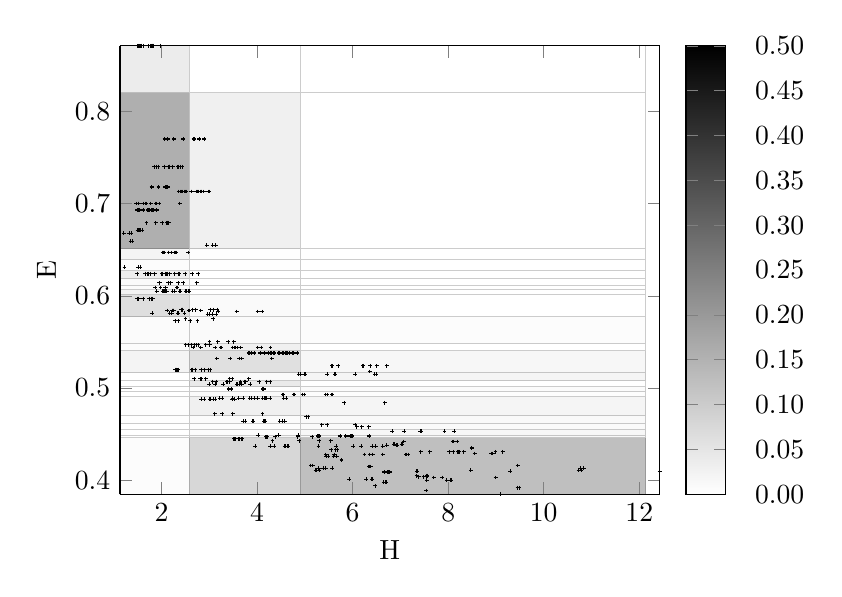
\begin{tikzpicture}
		\begin{axis}[
			view={0}{90},
			enlargelimits=0,
			zmin=0.0, zmax=1.0,
			xlabel=H,
			ylabel=E,
			colorbar,
			point meta min=0, point meta max=0.5,
			colormap={}{ gray(0cm)=(1); gray(1cm)=(0);},
			colorbar style={
			        ytick={0,0.05,...,0.5},
			        yticklabel style={
			            text width=2.5em,
			            align=right,
			            /pgf/number format/.cd,
			                fixed,
			                fixed zerofill
			        }
			    }
			]

			\addplot3[patch,shader=faceted,patch type=rectangle] coordinates {(1.1296,0.3850,0.0060) (2.5884,0.3850,0.0060) (2.5884,0.4460,0.0060) (1.1296,0.4460,0.0060)};
			\addplot3[patch,shader=faceted,patch type=rectangle] coordinates {(1.1296,0.4460,0.0000) (2.5884,0.4460,0.0000) (2.5884,0.4485,0.0000) (1.1296,0.4485,0.0000)};
			\addplot3[patch,shader=faceted,patch type=rectangle] coordinates {(1.1296,0.4485,0.0000) (2.5884,0.4485,0.0000) (2.5884,0.4555,0.0000) (1.1296,0.4555,0.0000)};
			\addplot3[patch,shader=faceted,patch type=rectangle] coordinates {(1.1296,0.4555,0.0000) (2.5884,0.4555,0.0000) (2.5884,0.4620,0.0000) (1.1296,0.4620,0.0000)};
			\addplot3[patch,shader=faceted,patch type=rectangle] coordinates {(1.1296,0.4620,0.0025) (2.5884,0.4620,0.0025) (2.5884,0.4705,0.0025) (1.1296,0.4705,0.0025)};
			\addplot3[patch,shader=faceted,patch type=rectangle] coordinates {(1.1296,0.4705,0.0040) (2.5884,0.4705,0.0040) (2.5884,0.4910,0.0040) (1.1296,0.4910,0.0040)};
			\addplot3[patch,shader=faceted,patch type=rectangle] coordinates {(1.1296,0.4910,0.0000) (2.5884,0.4910,0.0000) (2.5884,0.4960,0.0000) (1.1296,0.4960,0.0000)};
			\addplot3[patch,shader=faceted,patch type=rectangle] coordinates {(1.1296,0.4960,0.0000) (2.5884,0.4960,0.0000) (2.5884,0.5015,0.0000) (1.1296,0.5015,0.0000)};
			\addplot3[patch,shader=faceted,patch type=rectangle] coordinates {(1.1296,0.5015,0.0000) (2.5884,0.5015,0.0000) (2.5884,0.5085,0.0000) (1.1296,0.5085,0.0000)};
			\addplot3[patch,shader=faceted,patch type=rectangle] coordinates {(1.1296,0.5085,0.0000) (2.5884,0.5085,0.0000) (2.5884,0.5165,0.0000) (1.1296,0.5165,0.0000)};
			\addplot3[patch,shader=faceted,patch type=rectangle] coordinates {(1.1296,0.5165,0.0215) (2.5884,0.5165,0.0215) (2.5884,0.5410,0.0215) (1.1296,0.5410,0.0215)};
			\addplot3[patch,shader=faceted,patch type=rectangle] coordinates {(1.1296,0.5410,0.0055) (2.5884,0.5410,0.0055) (2.5884,0.5485,0.0055) (1.1296,0.5485,0.0055)};
			\addplot3[patch,shader=faceted,patch type=rectangle] coordinates {(1.1296,0.5485,0.0070) (2.5884,0.5485,0.0070) (2.5884,0.5775,0.0070) (1.1296,0.5775,0.0070)};
			\addplot3[patch,shader=faceted,patch type=rectangle] coordinates {(1.1296,0.5775,0.0645) (2.5884,0.5775,0.0645) (2.5884,0.6010,0.0645) (1.1296,0.6010,0.0645)};
			\addplot3[patch,shader=faceted,patch type=rectangle] coordinates {(1.1296,0.6010,0.0260) (2.5884,0.6010,0.0260) (2.5884,0.6070,0.0260) (1.1296,0.6070,0.0260)};
			\addplot3[patch,shader=faceted,patch type=rectangle] coordinates {(1.1296,0.6070,0.0085) (2.5884,0.6070,0.0085) (2.5884,0.6115,0.0085) (1.1296,0.6115,0.0085)};
			\addplot3[patch,shader=faceted,patch type=rectangle] coordinates {(1.1296,0.6115,0.0100) (2.5884,0.6115,0.0100) (2.5884,0.6190,0.0100) (1.1296,0.6190,0.0100)};
			\addplot3[patch,shader=faceted,patch type=rectangle] coordinates {(1.1296,0.6190,0.0325) (2.5884,0.6190,0.0325) (2.5884,0.6275,0.0325) (1.1296,0.6275,0.0325)};
			\addplot3[patch,shader=faceted,patch type=rectangle] coordinates {(1.1296,0.6275,0.0060) (2.5884,0.6275,0.0060) (2.5884,0.6390,0.0060) (1.1296,0.6390,0.0060)};
			\addplot3[patch,shader=faceted,patch type=rectangle] coordinates {(1.1296,0.6390,0.0210) (2.5884,0.6390,0.0210) (2.5884,0.6510,0.0210) (1.1296,0.6510,0.0210)};
			\addplot3[patch,shader=faceted,patch type=rectangle] coordinates {(1.1296,0.6510,0.1560) (2.5884,0.6510,0.1560) (2.5884,0.8205,0.1560) (1.1296,0.8205,0.1560)};
			\addplot3[patch,shader=faceted,patch type=rectangle] coordinates {(1.1296,0.8205,0.0370) (2.5884,0.8205,0.0370) (2.5884,0.8710,0.0370) (1.1296,0.8710,0.0370)};

			\addplot3[patch,shader=faceted,patch type=rectangle] coordinates {(2.5884,0.3850,0.0775) (4.9150,0.3850,0.0775) (4.9150,0.4460,0.0775) (2.5884,0.4460,0.0775)};
			\addplot3[patch,shader=faceted,patch type=rectangle] coordinates {(2.5884,0.4460,0.0150) (4.9150,0.4460,0.0150) (4.9150,0.4485,0.0150) (2.5884,0.4485,0.0150)};
			\addplot3[patch,shader=faceted,patch type=rectangle] coordinates {(2.5884,0.4485,0.0050) (4.9150,0.4485,0.0050) (4.9150,0.4555,0.0050) (2.5884,0.4555,0.0050)};
			\addplot3[patch,shader=faceted,patch type=rectangle] coordinates {(2.5884,0.4555,0.0040) (4.9150,0.4555,0.0040) (4.9150,0.4620,0.0040) (2.5884,0.4620,0.0040)};
			\addplot3[patch,shader=faceted,patch type=rectangle] coordinates {(2.5884,0.4620,0.0080) (4.9150,0.4620,0.0080) (4.9150,0.4705,0.0080) (2.5884,0.4705,0.0080)};
			\addplot3[patch,shader=faceted,patch type=rectangle] coordinates {(2.5884,0.4705,0.0290) (4.9150,0.4705,0.0290) (4.9150,0.4910,0.0290) (2.5884,0.4910,0.0290)};
			\addplot3[patch,shader=faceted,patch type=rectangle] coordinates {(2.5884,0.4910,0.0095) (4.9150,0.4910,0.0095) (4.9150,0.4960,0.0095) (2.5884,0.4960,0.0095)};
			\addplot3[patch,shader=faceted,patch type=rectangle] coordinates {(2.5884,0.4960,0.0025) (4.9150,0.4960,0.0025) (4.9150,0.5015,0.0025) (2.5884,0.5015,0.0025)};
			\addplot3[patch,shader=faceted,patch type=rectangle] coordinates {(2.5884,0.5015,0.0410) (4.9150,0.5015,0.0410) (4.9150,0.5085,0.0410) (2.5884,0.5085,0.0410)};
			\addplot3[patch,shader=faceted,patch type=rectangle] coordinates {(2.5884,0.5085,0.0100) (4.9150,0.5085,0.0100) (4.9150,0.5165,0.0100) (2.5884,0.5165,0.0100)};
			\addplot3[patch,shader=faceted,patch type=rectangle] coordinates {(2.5884,0.5165,0.0605) (4.9150,0.5165,0.0605) (4.9150,0.5410,0.0605) (2.5884,0.5410,0.0605)};
			\addplot3[patch,shader=faceted,patch type=rectangle] coordinates {(2.5884,0.5410,0.0295) (4.9150,0.5410,0.0295) (4.9150,0.5485,0.0295) (2.5884,0.5485,0.0295)};
			\addplot3[patch,shader=faceted,patch type=rectangle] coordinates {(2.5884,0.5485,0.0095) (4.9150,0.5485,0.0095) (4.9150,0.5775,0.0095) (2.5884,0.5775,0.0095)};
			\addplot3[patch,shader=faceted,patch type=rectangle] coordinates {(2.5884,0.5775,0.0105) (4.9150,0.5775,0.0105) (4.9150,0.6010,0.0105) (2.5884,0.6010,0.0105)};
			\addplot3[patch,shader=faceted,patch type=rectangle] coordinates {(2.5884,0.6010,0.0000) (4.9150,0.6010,0.0000) (4.9150,0.6070,0.0000) (2.5884,0.6070,0.0000)};
			\addplot3[patch,shader=faceted,patch type=rectangle] coordinates {(2.5884,0.6070,0.0000) (4.9150,0.6070,0.0000) (4.9150,0.6115,0.0000) (2.5884,0.6115,0.0000)};
			\addplot3[patch,shader=faceted,patch type=rectangle] coordinates {(2.5884,0.6115,0.0020) (4.9150,0.6115,0.0020) (4.9150,0.6190,0.0020) (2.5884,0.6190,0.0020)};
			\addplot3[patch,shader=faceted,patch type=rectangle] coordinates {(2.5884,0.6190,0.0000) (4.9150,0.6190,0.0000) (4.9150,0.6275,0.0000) (2.5884,0.6275,0.0000)};
			\addplot3[patch,shader=faceted,patch type=rectangle] coordinates {(2.5884,0.6275,0.0020) (4.9150,0.6275,0.0020) (4.9150,0.6390,0.0020) (2.5884,0.6390,0.0020)};
			\addplot3[patch,shader=faceted,patch type=rectangle] coordinates {(2.5884,0.6390,0.0015) (4.9150,0.6390,0.0015) (4.9150,0.6510,0.0015) (2.5884,0.6510,0.0015)};
			\addplot3[patch,shader=faceted,patch type=rectangle] coordinates {(2.5884,0.6510,0.0295) (4.9150,0.6510,0.0295) (4.9150,0.8205,0.0295) (2.5884,0.8205,0.0295)};
			\addplot3[patch,shader=faceted,patch type=rectangle] coordinates {(2.5884,0.8205,0.0000) (4.9150,0.8205,0.0000) (4.9150,0.8710,0.0000) (2.5884,0.8710,0.0000)};

			\addplot3[patch,shader=faceted,patch type=rectangle] coordinates {(4.9150,0.3850,0.1245) (12.1265,0.3850,0.1245) (12.1265,0.4460,0.1245) (4.9150,0.4460,0.1245)};
			\addplot3[patch,shader=faceted,patch type=rectangle] coordinates {(4.9150,0.4460,0.0135) (12.1265,0.4460,0.0135) (12.1265,0.4485,0.0135) (4.9150,0.4485,0.0135)};
			\addplot3[patch,shader=faceted,patch type=rectangle] coordinates {(4.9150,0.4485,0.0160) (12.1265,0.4485,0.0160) (12.1265,0.4555,0.0160) (4.9150,0.4555,0.0160)};
			\addplot3[patch,shader=faceted,patch type=rectangle] coordinates {(4.9150,0.4555,0.0090) (12.1265,0.4555,0.0090) (12.1265,0.4620,0.0090) (4.9150,0.4620,0.0090)};
			\addplot3[patch,shader=faceted,patch type=rectangle] coordinates {(4.9150,0.4620,0.0120) (12.1265,0.4620,0.0120) (12.1265,0.4705,0.0120) (4.9150,0.4705,0.0120)};
			\addplot3[patch,shader=faceted,patch type=rectangle] coordinates {(4.9150,0.4705,0.0185) (12.1265,0.4705,0.0185) (12.1265,0.4910,0.0185) (4.9150,0.4910,0.0185)};
			\addplot3[patch,shader=faceted,patch type=rectangle] coordinates {(4.9150,0.4910,0.0030) (12.1265,0.4910,0.0030) (12.1265,0.4960,0.0030) (4.9150,0.4960,0.0030)};
			\addplot3[patch,shader=faceted,patch type=rectangle] coordinates {(4.9150,0.4960,0.0070) (12.1265,0.4960,0.0070) (12.1265,0.5015,0.0070) (4.9150,0.5015,0.0070)};
			\addplot3[patch,shader=faceted,patch type=rectangle] coordinates {(4.9150,0.5015,0.0000) (12.1265,0.5015,0.0000) (12.1265,0.5085,0.0000) (4.9150,0.5085,0.0000)};
			\addplot3[patch,shader=faceted,patch type=rectangle] coordinates {(4.9150,0.5085,0.0200) (12.1265,0.5085,0.0200) (12.1265,0.5165,0.0200) (4.9150,0.5165,0.0200)};
			\addplot3[patch,shader=faceted,patch type=rectangle] coordinates {(4.9150,0.5165,0.0160) (12.1265,0.5165,0.0160) (12.1265,0.5410,0.0160) (4.9150,0.5410,0.0160)};
			\addplot3[patch,shader=faceted,patch type=rectangle] coordinates {(4.9150,0.5410,0.0000) (12.1265,0.5410,0.0000) (12.1265,0.5485,0.0000) (4.9150,0.5485,0.0000)};
			\addplot3[patch,shader=faceted,patch type=rectangle] coordinates {(4.9150,0.5485,0.0060) (12.1265,0.5485,0.0060) (12.1265,0.5775,0.0060) (4.9150,0.5775,0.0060)};
			\addplot3[patch,shader=faceted,patch type=rectangle] coordinates {(4.9150,0.5775,0.0000) (12.1265,0.5775,0.0000) (12.1265,0.6010,0.0000) (4.9150,0.6010,0.0000)};
			\addplot3[patch,shader=faceted,patch type=rectangle] coordinates {(4.9150,0.6010,0.0000) (12.1265,0.6010,0.0000) (12.1265,0.6070,0.0000) (4.9150,0.6070,0.0000)};
			\addplot3[patch,shader=faceted,patch type=rectangle] coordinates {(4.9150,0.6070,0.0000) (12.1265,0.6070,0.0000) (12.1265,0.6115,0.0000) (4.9150,0.6115,0.0000)};
			\addplot3[patch,shader=faceted,patch type=rectangle] coordinates {(4.9150,0.6115,0.0000) (12.1265,0.6115,0.0000) (12.1265,0.6190,0.0000) (4.9150,0.6190,0.0000)};
			\addplot3[patch,shader=faceted,patch type=rectangle] coordinates {(4.9150,0.6190,0.0000) (12.1265,0.6190,0.0000) (12.1265,0.6275,0.0000) (4.9150,0.6275,0.0000)};
			\addplot3[patch,shader=faceted,patch type=rectangle] coordinates {(4.9150,0.6275,0.0000) (12.1265,0.6275,0.0000) (12.1265,0.6390,0.0000) (4.9150,0.6390,0.0000)};
			\addplot3[patch,shader=faceted,patch type=rectangle] coordinates {(4.9150,0.6390,0.0000) (12.1265,0.6390,0.0000) (12.1265,0.6510,0.0000) (4.9150,0.6510,0.0000)};
			\addplot3[patch,shader=faceted,patch type=rectangle] coordinates {(4.9150,0.6510,0.0000) (12.1265,0.6510,0.0000) (12.1265,0.8205,0.0000) (4.9150,0.8205,0.0000)};
			\addplot3[patch,shader=faceted,patch type=rectangle] coordinates {(4.9150,0.8205,0.0000) (12.1265,0.8205,0.0000) (12.1265,0.8710,0.0000) (4.9150,0.8710,0.0000)};

			\addplot3[mark=+, draw=none, mark size=0.7, jitter = 0.3] coordinates {
(4.090,0.538,1) (4.967,0.469,1) (4.967,0.469,1) (6.062,0.458,1) (6.062,0.458,1) (6.062,0.458,1) (5.561,0.524,1) (5.950,0.524,1) (6.082,0.524,1) (6.592,0.524,1) (6.347,0.524,1) (6.227,0.524,1) (5.451,0.524,1) (4.707,0.538,1) (4.462,0.538,1) (4.499,0.538,1) (4.499,0.538,1) (4.258,0.538,1) (3.796,0.538,1) (3.796,0.538,1) (3.798,0.538,1) (4.012,0.538,1) (3.977,0.538,1) (4.095,0.538,1) (4.400,0.538,1) (4.455,0.538,1) (4.682,0.538,1) (4.453,0.538,1) (4.455,0.538,1) (4.239,0.538,1) (4.233,0.538,1) (4.175,0.538,1) (3.990,0.538,1) (3.787,0.538,1) (3.760,0.538,1) (3.360,0.499,1) (3.378,0.499,1) (3.934,0.499,1) (3.847,0.499,1) (5.401,0.428,1) (5.401,0.428,1) (5.721,0.448,1) (5.721,0.448,1) (5.721,0.448,1) (5.721,0.448,1) (5.100,0.448,1) (5.100,0.448,1) (5.689,0.448,1) (5.870,0.448,1) (6.088,0.448,1) (6.815,0.439,1) (6.815,0.439,1) (6.815,0.439,1) (6.815,0.439,1) (7.320,0.410,1) (8.697,0.403,1) (9.188,0.410,1) (8.325,0.411,1) (7.815,0.453,1) (6.932,0.453,1) (7.225,0.453,1) (6.819,0.453,1) (7.226,0.453,1) (7.981,0.453,1) (9.223,0.416,1) (6.612,0.398,1) (6.612,0.398,1) (6.498,0.409,1) (6.498,0.409,1) (6.498,0.409,1) (5.287,0.413,1) (5.287,0.413,1) (5.287,0.413,1) (5.287,0.413,1) (4.252,0.437,1) (4.503,0.437,1) (4.052,0.437,1) (4.090,0.437,1) (5.014,0.437,1) (4.503,0.437,1) (5.401,0.426,1) (5.401,0.426,1) (5.401,0.426,1) (5.401,0.426,1) (4.779,0.449,1) (4.438,0.449,1) (4.427,0.449,1) (3.748,0.449,1) (3.422,0.489,1) (3.414,0.489,1) (3.092,0.489,1) (3.092,0.489,1) (3.666,0.464,1) (3.666,0.464,1) (3.615,0.464,1) (3.495,0.445,1) (3.495,0.445,1) (3.495,0.445,1) (3.495,0.445,1) (3.495,0.445,1) (2.778,0.520,1) (2.856,0.520,1) (2.715,0.520,1) (2.715,0.520,1) (2.421,0.520,1) (2.107,0.520,1) (2.211,0.520,1) (2.122,0.520,1) (2.433,0.520,1) (2.545,0.520,1) (2.778,0.520,1) (2.678,0.547,1) (2.353,0.547,1) (2.548,0.547,1) (2.256,0.547,1) (2.463,0.547,1) (2.730,0.547,1) (2.747,0.547,1) (2.478,0.547,1) (2.759,0.547,1) (2.258,0.581,1) (2.197,0.581,1) (2.087,0.581,1) (1.944,0.581,1) (2.006,0.581,1) (1.993,0.581,1) (1.757,0.581,1) (1.788,0.624,1) (1.813,0.624,1) (1.980,0.624,1) (2.119,0.624,1) (2.271,0.624,1) (2.327,0.624,1) (2.470,0.624,1) (2.346,0.624,1) (2.111,0.624,1) (1.967,0.624,1) (1.850,0.624,1) (1.669,0.624,1) (1.669,0.624,1) (1.612,0.624,1) (1.439,0.624,1) (1.322,0.871,1) (1.412,0.871,1) (1.346,0.871,1) (1.419,0.871,1) (1.517,0.871,1) (1.461,0.871,1) (1.530,0.871,1) (1.526,0.871,1) (1.618,0.871,1) (1.592,0.871,1) (1.610,0.871,1) (1.623,0.871,1) (1.749,0.871,1) (1.746,0.871,1) (1.736,0.871,1) (1.877,0.605,1) (1.757,0.605,1) (1.766,0.871,1) (1.798,0.605,1) (1.971,0.605,1) (2.041,0.605,1) (2.162,0.605,1) (2.422,0.605,1) (2.283,0.605,1) (2.046,0.605,1) (2.426,0.605,1) (2.100,0.605,1) (2.263,0.605,1) (2.426,0.605,1) (2.389,0.605,1) (2.596,0.510,1) (2.646,0.510,1) (2.702,0.510,1) (3.132,0.510,1) (3.555,0.510,1) (3.317,0.510,1) (2.915,0.510,1) (2.829,0.488,1) (2.741,0.488,1) (2.598,0.488,1) (2.701,0.488,1) (2.847,0.488,1) (2.988,0.488,1) (3.280,0.488,1) (3.199,0.488,1) (3.789,0.437,1) (4.567,0.437,1) (4.567,0.437,1) (6.480,0.437,1) (6.480,0.437,1) (6.480,0.437,1) (6.220,0.401,1) (6.220,0.401,1) (5.648,0.422,1) (7.309,0.404,1) (7.309,0.404,1) (7.309,0.404,1) (7.653,0.403,1) (7.653,0.403,1) (6.270,0.415,1) (6.270,0.415,1) (5.118,0.416,1) (5.118,0.416,1) (3.945,0.489,1) (4.355,0.489,1) (4.355,0.489,1) (4.239,0.489,1) (3.875,0.489,1) (3.877,0.489,1) (3.665,0.489,1) (3.653,0.489,1) (3.945,0.489,1) (3.587,0.489,1) (3.945,0.489,1) (3.112,0.550,1) (3.421,0.550,1) (2.889,0.550,1) (3.363,0.550,1) (2.862,0.507,1) (3.048,0.507,1) (3.272,0.507,1) (3.272,0.507,1) (2.894,0.504,1) (2.894,0.504,1) (3.216,0.504,1) (3.216,0.504,1) (3.375,0.504,1) (3.375,0.504,1) (3.671,0.504,1) (3.671,0.504,1) (3.838,0.507,1) (3.652,0.507,1) (3.652,0.507,1) (3.652,0.507,1) (4.148,0.507,1) (4.148,0.507,1) (6.190,0.428,1) (6.190,0.428,1) (6.336,0.428,1) (6.336,0.428,1) (7.035,0.428,1) (7.035,0.428,1) (7.955,0.431,1) (7.955,0.431,1) (8.056,0.431,1) (8.056,0.431,1) (7.827,0.431,1) (7.827,0.431,1) (7.397,0.431,1) (7.397,0.431,1) (8.907,0.431,1) (8.907,0.431,1) (9.220,0.392,1) (9.220,0.392,1) (6.336,0.394,1) (1.801,0.647,1) (1.895,0.647,1) (2.011,0.647,1) (2.112,0.647,1) (2.140,0.647,1) (2.288,0.647,1) (2.079,0.647,1) (1.930,0.647,1) (1.986,0.647,1) (2.133,0.647,1) (2.422,0.575,1) (2.872,0.575,1) (3.917,0.464,1) (4.429,0.464,1) (4.429,0.464,1) (3.917,0.464,1) (4.367,0.464,1) (4.078,0.447,1) (4.267,0.447,1) (4.787,0.447,1) (4.863,0.447,1) (4.140,0.447,1) (4.101,0.443,1) (4.695,0.443,1) (5.245,0.443,1) (5.212,0.443,1) (5.885,0.401,1) (7.307,0.400,1) (7.307,0.389,1) (9.089,0.385,1) (7.317,0.405,1) (7.317,0.405,1) (7.317,0.405,1) (5.117,0.411,1) (5.117,0.411,1) (5.117,0.411,1) (5.503,0.437,1) (5.503,0.437,1) (5.960,0.437,1) (5.960,0.437,1) (6.320,0.437,1) (7.828,0.400,1) (7.828,0.400,1) (7.828,0.400,1) (5.492,0.433,1) (5.492,0.433,1) (5.492,0.433,1) (4.022,0.472,1) (3.370,0.472,1) (3.099,0.472,1) (3.183,0.472,1) (3.317,0.544,1) (3.103,0.544,1) (2.519,0.544,1) (2.640,0.544,1) (2.834,0.544,1) (3.263,0.544,1) (3.602,0.544,1) (3.945,0.544,1) (3.999,0.544,1) (4.032,0.544,1) (3.533,0.544,1) (4.002,0.544,1) (4.540,0.493,1) (4.540,0.493,1) (4.721,0.493,1) (4.721,0.493,1) (4.721,0.493,1) (5.416,0.493,1) (5.416,0.493,1) (5.416,0.493,1) (5.215,0.460,1) (5.215,0.460,1) (5.874,0.460,1) (6.641,0.438,1) (6.641,0.438,1) (6.458,0.515,1) (6.458,0.515,1) (5.985,0.515,1) (5.231,0.515,1) (5.615,0.515,1) (4.812,0.515,1) (4.812,0.515,1) (4.812,0.515,1) (7.038,0.442,1) (6.267,0.518,1) (5.732,0.484,1) (6.465,0.484,1) (8.014,0.442,1) (8.014,0.442,1) (8.535,0.429,1) (8.344,0.435,1) (8.792,0.429,1) (8.792,0.429,1) (10.710,0.411,1) (10.710,0.411,1) (12.127,0.410,1) (10.586,0.413,1) (10.586,0.413,1) (2.122,0.770,1) (2.505,0.770,1) (2.723,0.770,1) (2.509,0.770,1) (2.518,0.770,1) (2.296,0.770,1) (2.104,0.770,1) (1.905,0.770,1) (1.905,0.718,1) (1.613,0.718,1) (1.752,0.718,1) (1.511,0.631,1) (1.333,0.631,1) (1.357,0.631,1) (1.202,0.631,1) (1.169,0.631,1) (1.130,0.668,1) (1.174,0.668,1) (1.137,0.668,1) (1.316,0.671,1) (1.345,0.671,1) (1.358,0.671,1) (1.386,0.671,1) (1.386,0.671,1) (1.417,0.671,1) (1.519,0.671,1) (1.580,0.700,1) (1.533,0.700,1) (1.440,0.700,1) (1.426,0.700,1) (1.467,0.700,1) (1.518,0.700,1) (1.589,0.700,1) (1.728,0.700,1) (1.927,0.700,1) (2.168,0.700,1) (1.770,0.700,1) (1.791,0.693,1) (1.782,0.693,1) (1.726,0.693,1) (1.677,0.693,1) (1.633,0.693,1) (1.490,0.693,1) (1.500,0.693,1) (1.589,0.693,1) (1.574,0.693,1) (1.639,0.693,1) (1.703,0.693,1) (1.607,0.693,1) (1.425,0.693,1) (1.178,0.659,1) (1.285,0.659,1) (1.455,0.597,1) (1.466,0.597,1) (1.413,0.597,1) (1.528,0.597,1) (1.554,0.597,1) (1.589,0.597,1) (1.658,0.693,1) (1.835,0.679,1) (1.819,0.679,1) (1.647,0.679,1) (1.803,0.679,1) (1.794,0.718,1) (1.859,0.718,1) (1.875,0.718,1) (1.951,0.614,1) (2.022,0.614,1) (2.063,0.584,1) (1.910,0.679,1) (1.998,0.584,1) (1.863,0.679,1) (1.936,0.679,1) (1.968,0.679,1) (2.053,0.584,1) (2.088,0.584,1) (2.200,0.584,1) (2.316,0.713,1) (2.222,0.713,1) (2.125,0.740,1) (2.003,0.740,1) (1.914,0.740,1) (1.821,0.740,1) (1.817,0.740,1) (1.866,0.740,1) (2.065,0.740,1) (2.005,0.740,1) (1.978,0.740,1) (1.896,0.740,1) (1.988,0.740,1) (2.072,0.740,1) (2.198,0.740,1) (2.262,0.713,1) (2.185,0.713,1) (2.324,0.713,1) (2.355,0.713,1) (2.368,0.713,1) (2.453,0.713,1) (2.496,0.713,1) (2.436,0.713,1) (2.581,0.713,1) (2.779,0.713,1) (2.783,0.713,1) (2.717,0.713,1) (2.598,0.713,1) (2.567,0.713,1) (2.734,0.713,1) (2.802,0.713,1) (2.963,0.655,1) (3.067,0.655,1) (2.872,0.655,1) (2.540,0.584,1) (2.908,0.580,1) (2.824,0.580,1) (3.033,0.580,1) (3.099,0.532,1) (2.897,0.580,1) (2.533,0.614,1) (2.430,0.584,1) (2.206,0.584,1) (2.305,0.614,1) (2.101,0.614,1) (2.171,0.614,1) (1.951,0.614,1) (3.424,0.532,1) (3.332,0.532,1) (3.411,0.532,1) (4.098,0.532,1) (3.724,0.583,1) (3.992,0.583,1) (3.546,0.583,1) (3.152,0.583,1) (1.821,0.609,1) (1.755,0.609,1) (1.823,0.609,1) (1.868,0.609,1) (2.110,0.609,1) (2.382,0.585,1) (2.382,0.585,1) (2.799,0.585,1) (2.799,0.585,1) (2.893,0.585,1) (2.409,0.585,1) (2.400,0.585,1) (2.498,0.585,1) (2.479,0.573,1) (2.288,0.573,1) (2.167,0.573,1) (2.389,0.573,1) (2.505,0.573,1) };
		\end{axis}
	\end{tikzpicture}

  \caption{
    The discretization policy for variables $H$ and $E$ on the learned network in Figure~\ref{fig:housing_graph_2}.
    The number of discretization intervals for $H$ is less than it was for the fixed network structure in Figure~\ref{fig:housing_exp1_distr_8_5}, but the discretization policy still matches the raw data.
  }
  \label{fig:housing_exp2_distr_8_5}
\end{figure}

\subsection{Discussion}
\label{subsec:discuss_exp}

\begin{figure}[ht]
\centering
  % model_pca.tex
%
% Copyright (C) 2012 Jaakko Luttinen
%
% This file may be distributed and/or modified
%
% 1. under the LaTeX Project Public License and/or
% 2. under the GNU General Public License.
%
% See the files LICENSE_LPPL and LICENSE_GPL for more details.

% PCA model

%\beginpgfgraphicnamed{model-pca}
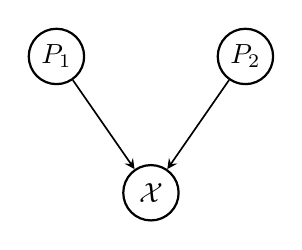
\begin{tikzpicture}[
      nodes={
        draw=black!20, thick, fill=white, font=\normalsize,
        minimum width=2.5em, minimum height=2em
      },
      rounded corners, semithick, >=stealth
      ]

  % Define nodes
  \node[latent]                               (y) {$\cX$};
  \node[latent, above=of y, xshift=-1.2cm] (p1) {$P_1$};
  \node[latent, above=of y, xshift=1.2cm]  (p2) {$P_2$};

  % Connect the nodes
  \edge {p1,p2} {y} ;

  % Plates
  %\plate {} {(p1)(p2)(p3)(y)} {$Factor_1$} ;
  %\plate {yx} {(y)(s11)(s12)(c2)} {$Factor_2$};
  %\plate {} {(y)(s2)(c1)(yx.north west)(yx.south west)} {$Factor_3$} ;
  %\plate {} {(w)(y)(yx.north west)(yx.south west)} {$M$} ;

\end{tikzpicture}
%\endpgfgraphicnamed

%%% Local Variables:
%%% mode: tex-pdf
%%% TeX-master: "example"
%%% End:

  \caption{A simple Bayesian network that is used to demonstrate the sensitivity of the three methods}
  \label{fig:exp_discuss}
\end{figure}

To quantatively discuss the sensitivity of the three methods to the number of discretization intervals, consider the Bayesian network in Figure~\ref{fig:exp_discuss}, where $\cX$ is continuous and $P_1$ and $P_2$ are discrete.
If $\Pa_{\cX} = \curly{P_1, P_2}$ and $D_{\cX} = \curly{1.0,2.0,3.0, \ldots n}$, then the corresponding objective functions for the three discretization methods are:

\begin{small}
  \begin{equation}
  \begin{aligned}
  f_{\text{MDL}} & = \overbrace{Z_1 \cdot k + \ln(k) + \ln {{n +k - 1}\choose{k -1}} }^{\text{Penalty Term}}+   \overbrace{\rule{0pt}{1.35em} \ln(N) \cdot I(X^*, \Pa_X)}^{\text{Edge Position Term}} \\
  f_{\text{Bayesian}} &= \overbrace{\rule{0pt}{1.85em}  Z_2 \cdot k + \sum_{i=1}^k \ln {{\gamma_i + J_P - 1}\choose{J_P -1}}}^{\text{Penalty Term}} + \overbrace{\sum^k_{i=1} \ln \left(   {{\gamma_i !}\over{n^{(P)}_{i,1}! n^{(P)}_{i,2}! \cdots n^{(P)}_{i,J_P}!    }} \right) }^{\text{Edge Position Term}}\\
  f_{\text{Heuristic}} &= \overbrace{Z_2 \cdot k + \sum_{i=1}^k \ln {{\gamma_i + J_{P_1} - 1}\choose{J_{P_1} -1}} + \sum_{i=1}^k \ln {{\gamma_i + J_{P_2} - 1}\choose{J_{P_2} -1}} }^{\text{Penalty Term}}+\\
  & \overbrace{\sum^k_{i=1}  \left[ \ln \left(   {{\gamma_i !}\over{n^{(P_1)}_{i,1}! n^{(P_1)}_{i,2}! \cdots n^{(P_1)}_{i,J_{P_1}}    }} \right)  + \ln \left(   {{\gamma_i !}\over{n^{(P_2)}_{i,1}! n^{(P_2)}_{i,2} \cdots n^{(P_2)}_{i,J_{P_2}} }} \right) \right]}^{\text{Edge Position Term}}
  \end{aligned}\text{,}
  \end{equation}
\end{small}

\noindent
where $Z_1$ and $Z_2$ are constant over discretizations, $k$ is the number of discretization intervals, and $I\paren{A, B} = \sum_{a,b} \hat{P}(a,b) \ln\frac{\hat{P}(a,b)}{\hat{P}(a)\hat{P}(b)}$ is the mutual information based on estimated probability1ies.
Note that the third term of $f_\text{MDL}$ had been approximated using $H(p)$ (see Equation~\ref{eqn:MDL}) in the original work by \cite{Friedman_1996} but here is written without that approximation.

The sensitivities of each method to the discretization edges are captured in the edge position terms, as the penalty terms are similar across methods.
The value of the edge position term for MDL is primarly determined by the mutual information, which varies less severely than the corresponding terms for the Bayesian methods.
The MDL term uses emperical probability distributions, based off of ratios of counts, whereas the Bayesian methods use factorial terms, and thus vary less severely.
Futhermore, the term for the heuristic Bayesian method varies more aggresively than the term for the optimal Bayesian method, as it has two terms.
The MDL method is thus the least sensitive to the discretization edges and the heuristic Bayesian method is over-sensitive.
This sensitivity gives rise to the relative performance of each method in the experiments conducted above.

%%%%%%%%%%%%%%%%%%%%%%%%%%%%%%%%%%%%%%%%%%%%%%%%%%%%%%%%%%%%%%%%%%%%%%%%%%%%%%%%%%%%%%
\section{Conclusion}
This paper introduced a principled discretization method for continuous variables in Bayesian networks with quadratic complexity instead of the cubic complexity of other standard techniques.
Emperical demonstrations show that the proposed method is superior to the state of the art.
In addition, this paper shows how to incorporate existing methods into the structure learning process to discretize all continuous variables and simultaneously learn Bayesian network structures.
The proposed method was incorporated and its superior performance was empirically demonstrated.
\todo{All software is publically available to support discretization research.}

The methods developed in this paper increase the accuracy of Bayesian networks learned on datasets with continuous and mixed variables.
An automated process for simultaneously constructing Bayesian networks and discretization policies is appearing because of the potential to significantly reduce development time and cost.
Future work will investigate edge positions at locations other than the midpoints between samples and using different discretization policies for the same variable in different conditional probablity distributions.

%\begin{acknowledgements}
%If you'd like to thank anyone, place your comments here
%and remove the percent signs.
%\end{acknowledgements}

% BibTeX users please use one of
%\bibliographystyle{spbasic}      % basic style, author-year citations
%\bibliographystyle{spmpsci}      % mathematics and physical sciences
%\bibliographystyle{spphys}       % APS-like style for physics
%\bibliography{}   % name your BibTeX data base

% Non-BibTeX users please use
%\begin{thebibliography}{}
\bibliographystyle{spbasic}
\bibliography{my_bib}

%%%%%%%%%%%%%%%%%%%%%%%%%%%%%%%%%%%%%%%%%%%%%%%%%%%%%%%%%%%%%%%%%%%%%%%%%%%%%%%%%%%%%%

\section*{Appendix}

\begin{algorithm}
  \caption{ Calculation of $h(u,v)$ for all $u \leq v$}
  \label{alg:h}
  \begin{algorithmic}[1]
  \State Initialize $H$ as an $N \times N$ matrix such that all elements are 0.
  \State $count_p$ is an $N \times N \times \|\Pa_X\|$ matrix such that $count_p [u,v,w]$ is the number of instances from $x_u$ to $x_v$ with $w$th value of $\Pa_X$. This matrix can be calculated in $O(\|\Pa_X\| \cdot N^2)$
  \For {$u = 1$ to $N$}
    \For {$v = u$ to $N$}
      \State $H(u,v) \leftarrow H(u,v) + \ln((v-u + J_p)!) - \ln((J_p -1)!)$
      \For {$w = 1$ to $\|\Pa_X\|$}
        \State $H(u,v) \leftarrow H(u,v) - \ln( count_p(u,v,w)!)$
      \EndFor
    \EndFor
  \EndFor
  \For {$j = 1$ to $n_c$}
    \State \todo{XXX}
  \EndFor
  \end{algorithmic}
\end{algorithm}

\end{document}
% end of file template.tex

